\documentclass[compress, 10pt]{beamer}
\usepackage{nuaabeamer}

\usepackage{graphics}

\usepackage{frame}
\usepackage{pgf}
\usepackage[UTF8, noindent]{ctex}
\usepackage{times}
\usepackage{amsmath}
\usepackage{algorithm}
\usepackage[noend]{algpseudocode}
\usefonttheme{professionalfonts}
\usepackage{listings}
\usepackage{color}
\usepackage{xcolor}
\lstset{
    language=C++,
    basicstyle=\tt,
    keywordstyle=\color{purple}\bfseries,
    identifierstyle=\color{brown!80!black},
    commentstyle=\color{gray}
    showstringspaces=false,
    % tiny font
    % basicstyle=\tiny,
    numbers=left,
    breaklines=true,
}

\usepackage{tikz}
\usetikzlibrary{shapes,arrows,positioning,calc}
\usepackage{pgfplots}
\usepackage{pgfplotstable}

\usepackage{caption}
\setbeamertemplate{caption}[numbered]{}

\usepackage[backend=bibtex,style=ieee,sorting=none]{biblatex}
% \addbibresource{ref.bib}
\setbeamerfont{footnote}{size=\tiny}

\usepackage{subfigure}

\makeatletter
\let\@@magyar@captionfix\relax
\makeatother

\newcommand{\Title}{SPH方法实现报告三}
\newcommand{\Reporter}{包晨宇}
\newcommand{\Instructor}{吕宏强}
\newcommand{\Institute}{南京航空航天大学}

\begin{document}

\captionsetup[figure]{font=footnotesize,labelfont=footnotesize}

\title{\Title}
\author{汇报人:\Reporter \\ \vspace{1em} 指导人:\Instructor}
\date{\today}
\institute{\Institute}

\begin{frame}
    \begin{figure}[H]
        \centering
        
\includegraphics[width=0.2\textwidth]{logo.pdf}
    \end{figure}
    \maketitle
\end{frame}

\section*{目录}
\begin{frame}
    \frametitle{\secname}
    \tableofcontents[sections={<1-5>}]
\end{frame}

\AtBeginSection[] {%在每一节前面加入目录显示当前节的目录结构
	\begin{frame}
		\frametitle{目录}
		\tableofcontents[currentsection,currentsubsection,hideothersubsections,sectionstyle=show/shaded,]
		\addtocounter{framenumber}{-1}  %目录页不计入页码
	\end{frame}
}

\section{SPH 方法回顾}

\begin{frame}
    一个物理场量 $A(\vec{r})$ 可以用其在空间中分布的加权积分得到:
    \begin{equation}
        A(\vec{r}) = \int A(\vec{r}^\prime) W(\vec{r} - \vec{r}^\prime, h) \mathrm{d} \vec{r}^\prime
    \end{equation}
    其中 $W(\vec{r} - \vec{r}^\prime, h)$ 是光滑核函数,$h$ 是光滑长度。
    这是一个与 $\delta(\vec{r})$ 相似的函数,但是具有有限的支撑域。
    一个物理量的核函数插值,仅由其在支撑域内的物理量决定。
    同时,该物理量梯度经分部积分和边界舍入,也可以表达为:
    \begin{equation}
        \nabla A(\vec{r}) = \int A(\vec{r}^\prime) \nabla W(\vec{r} - \vec{r}^\prime, h) \mathrm{d} \vec{r}^\prime
    \end{equation}
    在物理量被一颗颗粒子携带的时候,
    上述积分可以表示为对支撑域内所有粒子的加权求和:
    \begin{equation}
        \begin{aligned}
            A_i &= \sum_j \frac{m_j}{\rho_j} A_j W_{ij} \\
            \nabla A_i &= \sum_j \frac{m_j}{\rho_j} A_j \nabla W_{ij}
            \quad \nabla W_{ij} \parallel \vec{r}_{ij}
        \end{aligned}
    \end{equation}
\end{frame}

\begin{frame}
    虽然据此已经可以离散出含导数的物理方程,
    但精度并不高,
    因此多种离散形式被提出,其核心思想大致如下,
    对 $\nabla$ 算子外用指标 $i$ ,算子内用指标 $j$:
    \begin{equation}
        \begin{aligned}
            \phi \nabla A &= \nabla (\phi A) - A \nabla \phi\\
            &= \sum_j \frac{m_j}{\rho_j} \phi_j A_j \nabla W_{ij}
            - \sum_j \frac{m_j}{\rho_j} A_i \phi_j \nabla W_{ij}\\
            &= \sum_j \frac{m_j}{\rho_j} \phi_j (A_j - A_i) \nabla W_{ij}
        \end{aligned}
    \end{equation}
    比如对于项 $\rho\nabla\cdot \vec{v}$ 的离散形式如($\phi=\rho$):
    \begin{equation}
        \rho_i \nabla \cdot \vec{v}_i = -\sum_j m_j \vec{v}_{ij} \cdot \nabla W_{ij}
    \end{equation}
    而对于 $\frac{1}{\rho}\nabla p = \nabla \left(\frac{p}{\rho}\right) + \frac{p}{\rho^2}\nabla \rho$,
    则有形式如($\phi=\frac{1}{\rho}$):
    \begin{equation}
        \frac{1}{\rho_i}\nabla p_i = \sum_j m_j \left(\frac{p_i}{\rho_i^2} + \frac{p_j}{\rho_j^2}\right) \nabla W_{ij}
    \end{equation}
\end{frame}

\begin{frame}
    在 Lagrange 描述下,不可压流体的基本方程为,
    暂时不考虑能量方程。
    \begin{equation}
        \begin{aligned}
            \frac{\mathrm{d} \rho}{\mathrm{d} t} &= -\rho \nabla \cdot \vec{v} \\
            \frac{\mathrm{d} \vec{v}}{\mathrm{d} t} &= -\frac{1}{\rho} \nabla p + \vec{g} + \nu \nabla^2 \vec{v}\\
            \frac{\mathrm{d} \vec{x}}{\mathrm{d} t} &= \vec{v}
        \end{aligned}
    \end{equation}
    目前 SPH 方法广为使用的方式是弱可压 WCSPH 方法,
    其允许流体的密度在一定范围内变化。
    并且给出了状态方程如下:
    \begin{equation}
        p = \frac{c_0^2\rho_0}{\gamma}
        \left[\left(\frac{\rho}{\rho_0}\right)^\gamma - 1\right]=
        \frac{c_0^2\rho_0}{\gamma}
        \left[\left(1+\frac{\rho-\rho_0}{\rho_0}\right)^\gamma - 1\right]
    \end{equation}
    在 $\rho$ 变化不大时,方程可以退化为 $p=c_0^2(\rho-\rho_0)$。
\end{frame}

\begin{frame}
    根据光滑核函数插值,
    我们可以将 SPH 的控制方程离散成光滑核函数的插值形式:
    \begin{equation}
        \begin{aligned}
            \frac{\mathrm{d} \rho_i}{\mathrm{d} t} &= \rho_i \sum_j m_j \vec{v}_{ij} \cdot \nabla W_{ij} \\
            \frac{\mathrm{d} \vec{v}_i}{\mathrm{d} t} &= -\sum_j m_j \left(\frac{p_i}{\rho_i^2} + \frac{p_j}{\rho_j^2}\right) \nabla W_{ij} + \vec{g} + \nu \nabla^2 \vec{v}_i
        \end{aligned}
    \end{equation}
    其中粘性项的离散形式比较多样,
    各种参考文献中给出的结果不尽相同:
    \begin{equation}
        \nu \nabla^2 \vec{v}_i = 
        \sum_j m_j
        \frac{4 (\mu_i + \mu_j) \vec{r}_{ij}\cdot \nabla W_{ij}}{(\rho_i + \rho_j)^2 (r_{ij}^2 + 0.01h^2)}\vec{v}_{ij}
    \end{equation}
\end{frame}

\begin{frame}
    一种可能的推导过程如下,将某速度矢量作泰勒展开:
    \begin{equation}
        \vec{v}_i \approx
        \vec{v}_j + (\vec{r}_i - \vec{r}_j)\cdot \nabla\vec{v}_j
        \to
        \vec{v}_{ij} \approx \vec{r}_{ij}\cdot \nabla\vec{v}_j
    \end{equation}
    其中对二维情况,
    $\nabla \vec{v}_j$ 是一个 $2\times 2$ 的矩阵,
    \begin{equation}
        \nabla\vec{v}_j =
    \begin{bmatrix}
        \frac{\partial v_{j,x}}{\partial x} & \frac{\partial v_{j,y}}{\partial x} \\
        \frac{\partial v_{j,x}}{\partial y} & \frac{\partial v_{j,y}}{\partial y} 
    \end{bmatrix}
    \end{equation}
    进而导出:
        \begin{equation}
            \begin{aligned}
                \nabla^2\vec{v}_i &= [\nabla\cdot (\nabla\vec{v})]_i\\
                &\approx \sum_j \frac{m_j}{\rho_j} \nabla W_{ij}
                \cdot \nabla\vec{v}_j\\
            \end{aligned}
        \end{equation}
\end{frame}

\begin{frame}
    对于$\nabla W_{ij} = \frac{\vec{r}_{ij}}{r_{ij}}\frac{1}{h}W^\prime_{ij}$:
    \begin{equation}
        \vec{r}_{ij}\cdot W_{ij} = \frac{r_{ij}}{h}W^\prime_{ij}
    \end{equation}
    \begin{equation}
        \begin{aligned}
            \nabla^2\vec{v}_i &= 
        \sum_j \frac{m_j}{\rho_j} \frac{1}{h r_{ij}}W^\prime_{ij}
        (\vec{r}_{ij} \cdot \nabla\vec{v}_j)\\
        &=
        \sum_j \frac{m_j}{\rho_j} \frac{1}{h r_{ij}}W^\prime_{ij}\vec{v}_{ij}\\
        &=
        \sum_j \frac{m_j}{\rho_j} \frac{1}{r_{ij}^2} \frac{r_{ij}}{h}W^\prime_{ij}\vec{v}_{ij}\\
        &=
        \sum_j \frac{m_j}{\rho_j} \frac{\vec{r}_{ij}\cdot \nabla W_{ij}}{r_{ij}^2} \vec{v}_{ij}\\
        \end{aligned}
    \end{equation}
    为了避免奇异,在分母上添加项,我的推导和 SPhysics 中的形式一致:
    \begin{equation}
        \nabla^2\vec{v}_i = 
        \sum_j \frac{m_j}{\rho_j} \frac{\vec{r}_{ij}\cdot \nabla W_{ij}}{r_{ij}^2+0.01h^2} \vec{v}_{ij}
    \end{equation}
\end{frame}

\begin{frame}
    上述推导是我能够理解的也认为是正确的,
    但对于粘性项似乎文献中给出了千奇百怪的形式,
    有的甚至干脆直接差一个系数,比如 Jan Bender, 2020 给出的形式为:
    \begin{equation}
        \nabla^2\vec{v}_i =
        2(d+2)\sum_j
        \frac{m_j}{\rho_j}
        \frac{\vec{v}_{ij}\cdot \vec{r}_{ij}}{r_{ij}^2 + 0.01h^2}
        \nabla W_{ij}
    \end{equation}
    Colagrossi 和 Aristodemo 等给出的公式则为:
    \begin{equation}
        \nu_0 \nabla^2\vec{v}_i =
        \sum_j 
        \frac{4(d+2)\nu_0 \vec{v}_{ij}\cdot \vec{r}_{ij}}{(\rho_i + \rho_j)(r_{ij}^2 + 0.01h^2)}
        \nabla W_{ij}
    \end{equation}
    Price, 2012 则给出的公式为:
    \begin{equation}
        \nabla^2\vec{v}_i =
        -2\sum_j
        \frac{m_j}{\rho_j}
        \vec{v}_{ij}\frac{\vec{r}_{ij}\cdot\nabla W_{ij}}{r_{ij}^2+0.01h^2}
    \end{equation}
    这些推导都没有详尽的解释,看起来有点关系,
    但其实表达的含义完全不同。
    这也为后续的推导造成了比较大的影响,尤其是壁面摩擦。
\end{frame}

\begin{frame}
    \begin{algorithm}[H]
        \caption{WCSPH Simple Solver}
        \begin{algorithmic}[1]
            \State \textbf{Input:} $\rho_0, c, \nu, \vec{g}, \Delta t$ etc.
            \State \textbf{Output:} $\rho, \vec{v}, p$
            \While{current time step < total time step}
                \State neighbour = findNeighbour(particles, radius)
                \For{each neighbour $i,j$}
                    \State Update $\rho$ using $\frac{d\rho}{dt}= -\rho \nabla\cdot \vec{v}$
                \EndFor
                \For{each particle $i$}
                    \State Update $p$ using $p = c^2(\rho - \rho_0)+p_0$
                \EndFor
                \For{each neighbour $i,j$ (wall includes compulsive force)}
                    \State $\vec{f}_{\text{p}}= -\sum_j m_j \left(\frac{p_i}{\rho_i^2} + \frac{p_j}{\rho_j^2}\right) \nabla W_{ij}$
                    \State $\vec{f}_{\text{v}}= \sum_j m_j \frac{4 (\mu_i + \mu_j) \vec{r}_{ij}\cdot \nabla W_{ij}}{(\rho_i + \rho_j)^2 (r_{ij}^2 + 0.01h^2)}\vec{v}_{ij}$
                \EndFor
                \For{each particle $i$}
                    \State Update $\vec{v}$ to $\vec{v}^{n+1}$ with pressure using $\frac{d\vec{v}}{dt}= -\frac{1}{\rho}\nabla p+\frac{\mu}{\rho} \nabla^2 \vec{v}+\vec{g}$
                    \State Update $\vec{r}$ using $\frac{d\vec{r}}{dt}= \vec{v}$
                \EndFor
            \EndWhile
        \end{algorithmic}
    \end{algorithm}
\end{frame}
\section{边界以及环境设置}

\subsection{环境压力(背景压力)}

\begin{frame}
    \begin{figure}[H]
        \centering
        \subfigure[低压区]{
            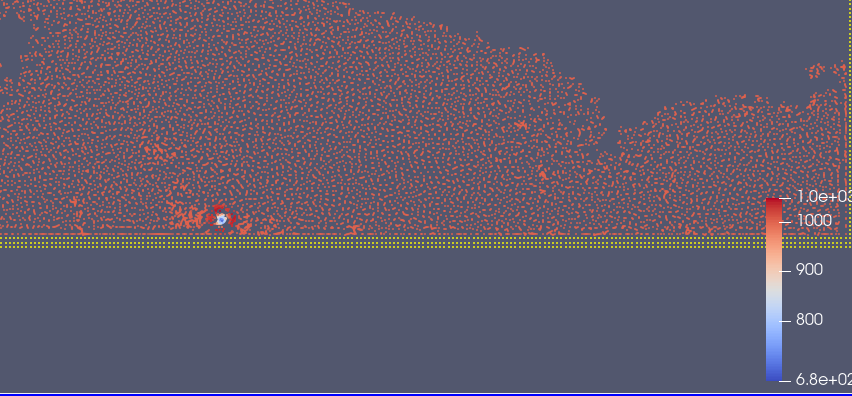
\includegraphics[width=0.6\textwidth]{images/low_pressure_field.png}
        }\\
        \subfigure[局部粒子打穿流场]{
            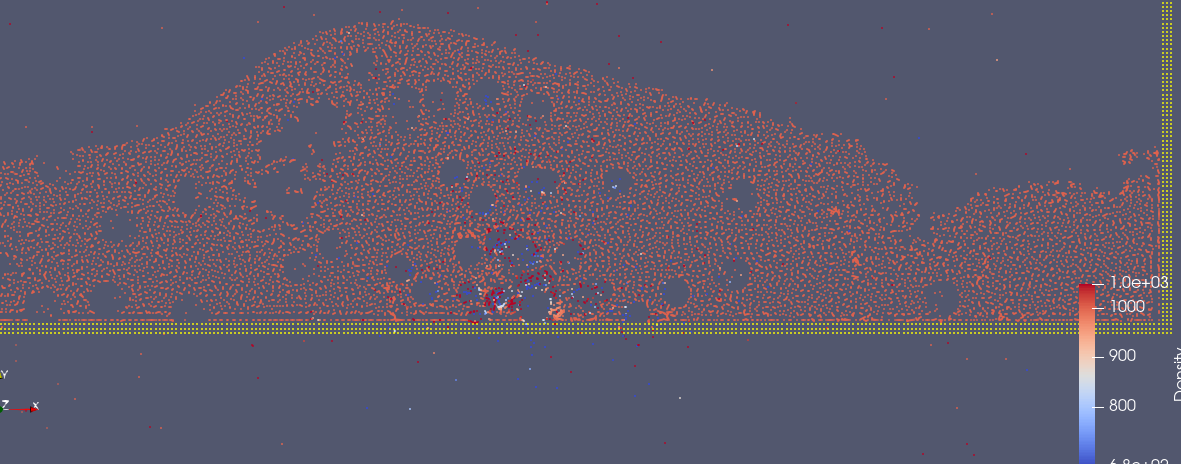
\includegraphics[width=0.6\textwidth]{images/emit_like_bullet.png}
        }
    \end{figure}
\end{frame}

\begin{frame}
    增加背景压力这件事情是不可行的,
    或者说在液柱垮塌问题中是不可行的。
    回顾压力项的核插值格式:
    \begin{equation}
        \left(\frac{1}{\rho}\nabla p\right)_i
        =
        \sum_j m_j
        \left(\frac{p_i}{\rho_i^2}+\frac{p_j}{\rho_j^2}\right)
        \nabla W_{ij}
    \end{equation}
    如果将背景压力 $p_0$ 加入到这个式子中,
    那么上述压力项就变成了:
    \begin{equation}
        \left(\frac{1}{\rho}\nabla p\right)_i
        =
        \sum_j m_j
        \left(\frac{p_i}{\rho_i^2}+\frac{p_j}{\rho_j^2}\right)
        \nabla W_{ij}
        +
        \sum_j m_j
        \left(\frac{p_0}{\rho_i^2}+\frac{p_0}{\rho_j^2}\right)
        \nabla W_{ij}
    \end{equation}
    \begin{figure}[H]
        \centering
        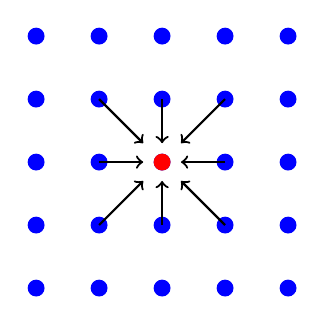
\begin{tikzpicture}
            % draw 5*5 particles
            \foreach \x in {0,1,2,3,4}
            \foreach \y in {0,1,2,3,4}
            {
                \filldraw[blue] (0.8*\x,0.8*\y) circle (0.1);
            }
            % filldraw the center particle as red
            \filldraw[red] (0.8*2,0.8*2) circle (0.1);
            % draw arrow towards the center particle from neighbour particles
            \foreach \x in {1,3}
            \foreach \y in {1,3}
            {
                \draw[->,thick] (0.8*\x,0.8*\y) -- ({0.8*\x + 0.7*0.8*(2-\x)}, {0.8*\y + 0.7*0.8*(2-\y)});
            }
            % draw arrow towards the center particle from neighbour particles up, down, left, right
            \foreach \x in {1,3}
            {
                \draw[->,thick] (0.8*\x,0.8*2) -- ({0.8*\x + 0.7*0.8*(2-\x)}, {0.8*2});
                \draw[->,thick] (0.8*2,0.8*\x) -- ({0.8*2}, {0.8*\x + 0.7*0.8*(2-\x)});
            }
        \end{tikzpicture}
    \end{figure}
\end{frame}

\begin{frame}
    如前图所述,
    当粒子致密的时候,
    会有大量的粒子向中心粒子施加压力,
    靠着足够多的邻域粒子产生的统计效应,
    背景压力会在这种情况下被互相抵消。
    反之,对于多相流问题,
    平白无故地增加背景压力会导致自由表面处背景压强项缺失,
    从而导致粒子的不稳定运动。
    \begin{figure}[H]
        \centering
        \begin{tikzpicture}
            % draw 5*5 particles
            \foreach \x in {0,1,2}
            \foreach \y in {0,1,2,3,4}
            {
                \filldraw[blue] (0.8*\x,0.8*\y) circle (0.1);
            }
            % filldraw the center particle as red
            \filldraw[red] (0.8*2,0.8*2) circle (0.1);
            % draw arrow towards the center particle from neighbour particles
            \foreach \x in {1,3}
            \foreach \y in {1,3}
            {
                \draw[->,thick] (0.8*\x,0.8*\y) -- ({0.8*\x + 0.7*0.8*(2-\x)}, {0.8*\y + 0.7*0.8*(2-\y)});
            }
            % draw arrow towards the center particle from neighbour particles up, down, left, right
            \foreach \x in {1,3}
            {
                \draw[->,thick] (0.8*\x,0.8*2) -- ({0.8*\x + 0.7*0.8*(2-\x)}, {0.8*2});
                \draw[->,thick] (0.8*2,0.8*\x) -- ({0.8*2}, {0.8*\x + 0.7*0.8*(2-\x)});
            }
            \foreach \x in {3,4}
            \foreach \y in {0,1,2,3,4}
            {
                \filldraw[gray] (0.8*\x,0.8*\y) circle (0.1);
            }
            \node[blue] at (-0.5,0.8*2) {水体};
            \node[gray] at (4,0.8*2) {气体};
        \end{tikzpicture}
    \end{figure}
    因此想要增加背景压力,
    正确的做法应该是同时增加气体相的粒子,
    让气体相的粒子在自由表面处产生压力,
    参与进整个流场的压力计算中。
    简言之,
    流域致密的时候可以加背景压力(但也不宜加太多),
    流域稀疏,有多相时,需要增加流相以平衡背景压力。
\end{frame}

\begin{frame}
    一种可能的修正方式是用 Monaghan 的方法,
    在压力项中添加一个斥力:
    \begin{equation}
        \vec{f}_i^p = 
        -\sum_j 
        m_j 
        \left(
            \frac{p_i}{\rho_i^2} + \frac{p_j}{\rho_j^2} + R_{ij}
        \right)\nabla W_{ij}
    \end{equation}
    $R_{ij}$ ($\Delta p$ 为初始粒子间距):
    \begin{equation}
        R_{ij} = 
        0.01
        \left(
            \frac{|p_i|}{\rho_i^2} + \frac{|p_j|}{\rho_j^2}
        \right)
        \frac{W(r_{ij}, h)}{W(\Delta p, h)}
    \end{equation}
    因为核函数是一个“高耸”的函数,因此在 $r_{ij}=\Delta p$ 时,
    压力项仅多了有限的 1\%,而在两粒子很靠近 $r_{ij}\to 0$ 时,
    该斥力项会迅速增大,从而避免了粒子的堆积。
    在实践中,该方法可以很好的解决粒子堆积造成的负压爆炸的问题, 
\end{frame}

\subsection{壁面力}

\begin{frame}
    经过前述描述,
    我们知道了背景压力的作用,
    因为壁面也是用粒子来描述实现的,
    我们可以将壁面力分为三部分:
    \begin{itemize}
        \item 壁面强制力,这部分采用的 Monaghan 的方法,本质上借鉴了接触力学中的概念。
        \item 壁面环境压力,该项仅在流体致密的问题中起作用,对于自由表面问题,不用加入该项。
        \item 壁面粘性*,这部分的引入问题比较大,我会在后续的算例中展示结果与曲线对比。
    \end{itemize}
    \begin{figure}[H]
        \centering
        \begin{tikzpicture}
            \draw[->,thick] (-0.1, 0) -- (3,0);
            \draw[->,thick] (0, -0.1) -- (0,3);
            % draw 1/x 
            \draw[domain=0.3:3,smooth,variable=\x,blue,thick=3] plot ({\x},{1/\x-1/3});
            \node at (3,1.5) {壁面强制力 $0.01\frac{c^2}{h}f(x_\perp)$};
        \end{tikzpicture}
    \end{figure}
\end{frame}

\begin{frame}
    壁面粘性在目前的算例中是存在问题的,
    这里给出一个简单的示意图:
    \begin{figure}[H]
        \begin{tikzpicture}
            \draw[-, thick] (0,0) -- (5,0);
            \node at (-0.5, 0) {壁面};
            \draw[gray] (2,0)--(2,-1)--(3,-1)--(3,0);
            \filldraw[gray] (2.5,-0.5) circle (0.1);
            \draw[blue] (2,0)--(2,1)--(3,1)--(3,0);
            \filldraw[blue] (2.5,0.5) circle (0.1);

            \node[gray] at (2.5, -1.5) {壁面粒子};
            \node[blue] at (2.5, 1.5) {流体粒子};

            \node at (7, 0) {$\vec{v}=0$:理想无滑移边界};
            \node[gray] at (7, -1) {$\vec{v}=0$:按零速度粒子处理的粘性边界};

            % denote wall boundary and wall particle's position -dr/2
            % use } to denote the -dr/2
            \draw[->,thick,red] (3.1,0) -- (3.1,-0.5) node[below] {$-\frac{\Delta p}{2}$};
            
            \draw[dashed] (0.5, 0.5) -- (0.5,-0.5) -- (1.5,-0.5) -- (1.5,0.5) -- (0.5,0.5);
            \filldraw (1,0) circle (0.1);
        \end{tikzpicture}
    \end{figure}
    如果将壁面粒子视作一般的速度为零的水体粒子纳入粘性计算,
    那其实并不能很好的描述壁面无滑移的情况。
    因为粒子客观存在体积,
    进而壁面粒子被埋入墙体 $\frac{\Delta p}{2}$ 的位置,
    真正速度为零的位置被深埋了一段距离。
    另一方面,
    流体粒子因为壁面强制力的原因,
    无法侵入壁面 $\frac{\Delta p}{2}$ 的位置,
    因此其质心始终存在速度,
    不可能贴在墙壁上不运动。

    后续算例的粘性,*会展示将壁面粒子抬高和不抬高 $\frac{\Delta p}{2}$ 的结果对比。
\end{frame}
\section{液柱垮塌算例}

\begin{frame}
    \begin{figure}[H]
        \centering
        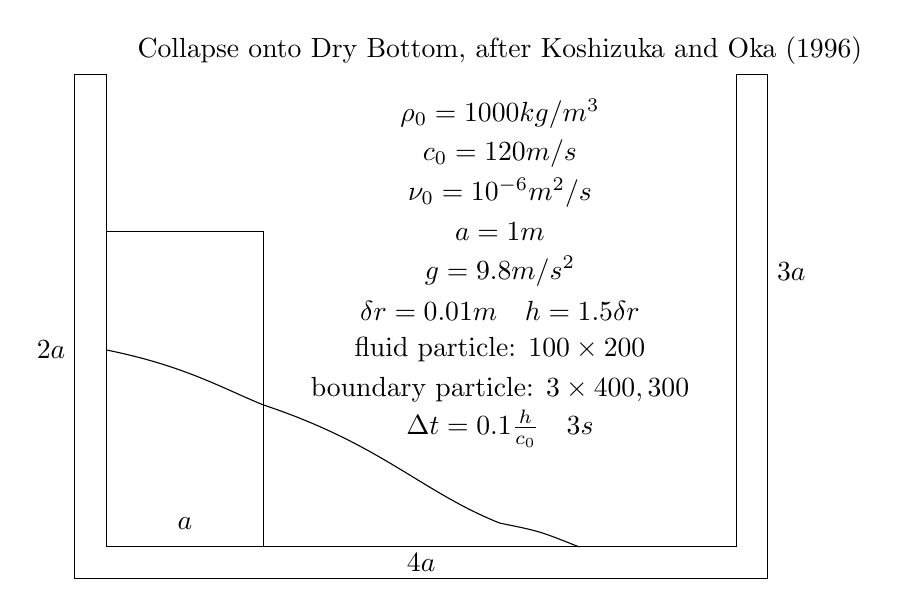
\begin{tikzpicture}
            \draw[-] (0,6)--(0,0)--(8,0)--(8,6);
            \draw[-] (0,6)--(-0.4,6)--(-0.4,-0.4)--(8.4,-0.4)--(8.4,6)--(8,6);
            \draw[-] (0,4)--(2,4)--(2,0);
            
            % arbitrary fluid surface at some time
            \draw (0,2.5) .. controls (1,2.3) and (1.5,2.0) .. (2,1.8) .. controls (3.5,1.3) and (4,0.7) .. (5,0.3) .. controls (5.5,0.2) .. (6,0);
            
            \node at (1,0.3) {$a$};
            \node at (4, -0.2) {$4a$};
            \node at (-0.7, 2.5) {$2a$};
            \node at (8.7, 3.5) {$3a$};

            \node at (5, 6.3) {Collapse onto Dry Bottom, after Koshizuka and Oka (1996)};
            \node at (5, 5.5) {$\rho_0=1000kg/m^3$};
            \node at (5, 5) {$c_0=120m/s$};
            \node at (5, 4.5) {$\nu_0=10^{-6}m^2/s$};
            \node at (5, 4) {$a=1m$};
            \node at (5, 3.5) {$g=9.8m/s^2$};
            \node at (5, 3) {$\delta r=0.01m\quad h=1.5\delta r$};
            \node at (5, 2.5) {fluid particle: $100\times 200$};
            \node at (5, 2) {boundary particle: $3\times 400,300$};
            \node at (5, 1.5) {$\Delta t=0.1\frac{h}{c_0}\quad 3s$};
        \end{tikzpicture}
    \end{figure}
\end{frame}

\begin{frame}
    \begin{figure}[H]
        \centering
        \subfigure[壁面粒子未垫高]{
            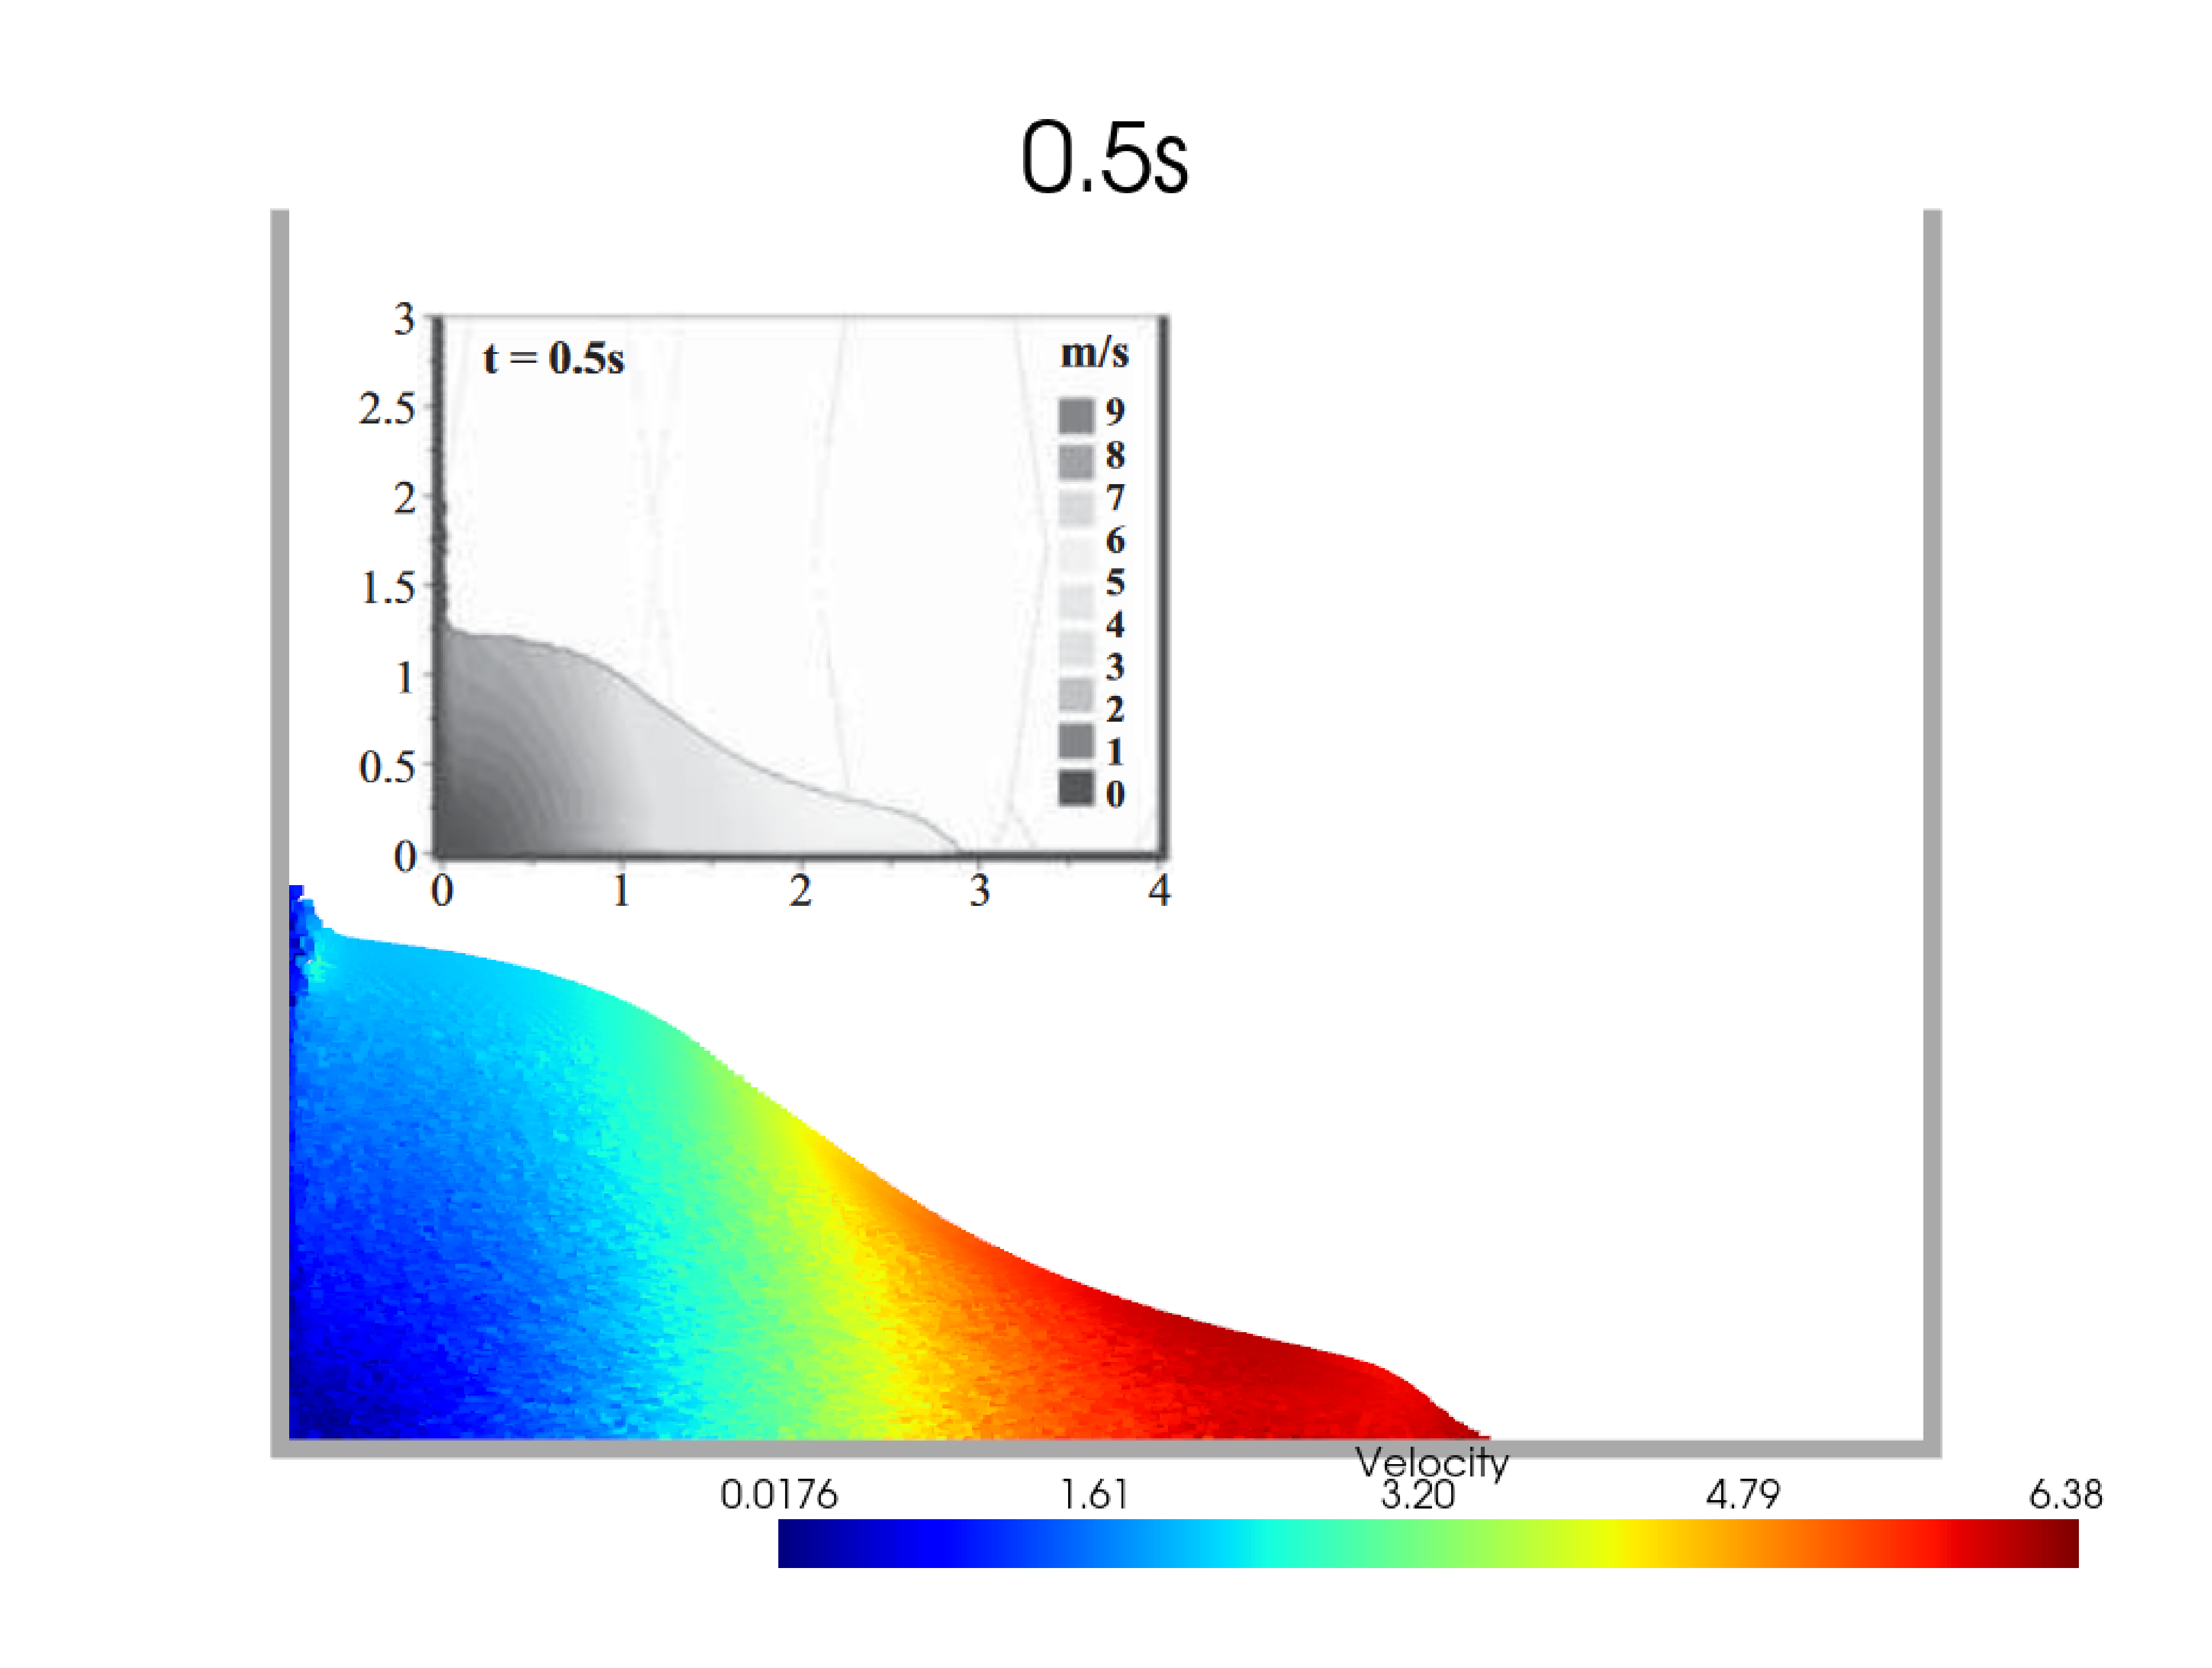
\includegraphics[width=0.47\textwidth]{images/CollapseDry/origin/collapse_dry05_combined.png}
        }
        \subfigure[壁面粒子垫高]{
            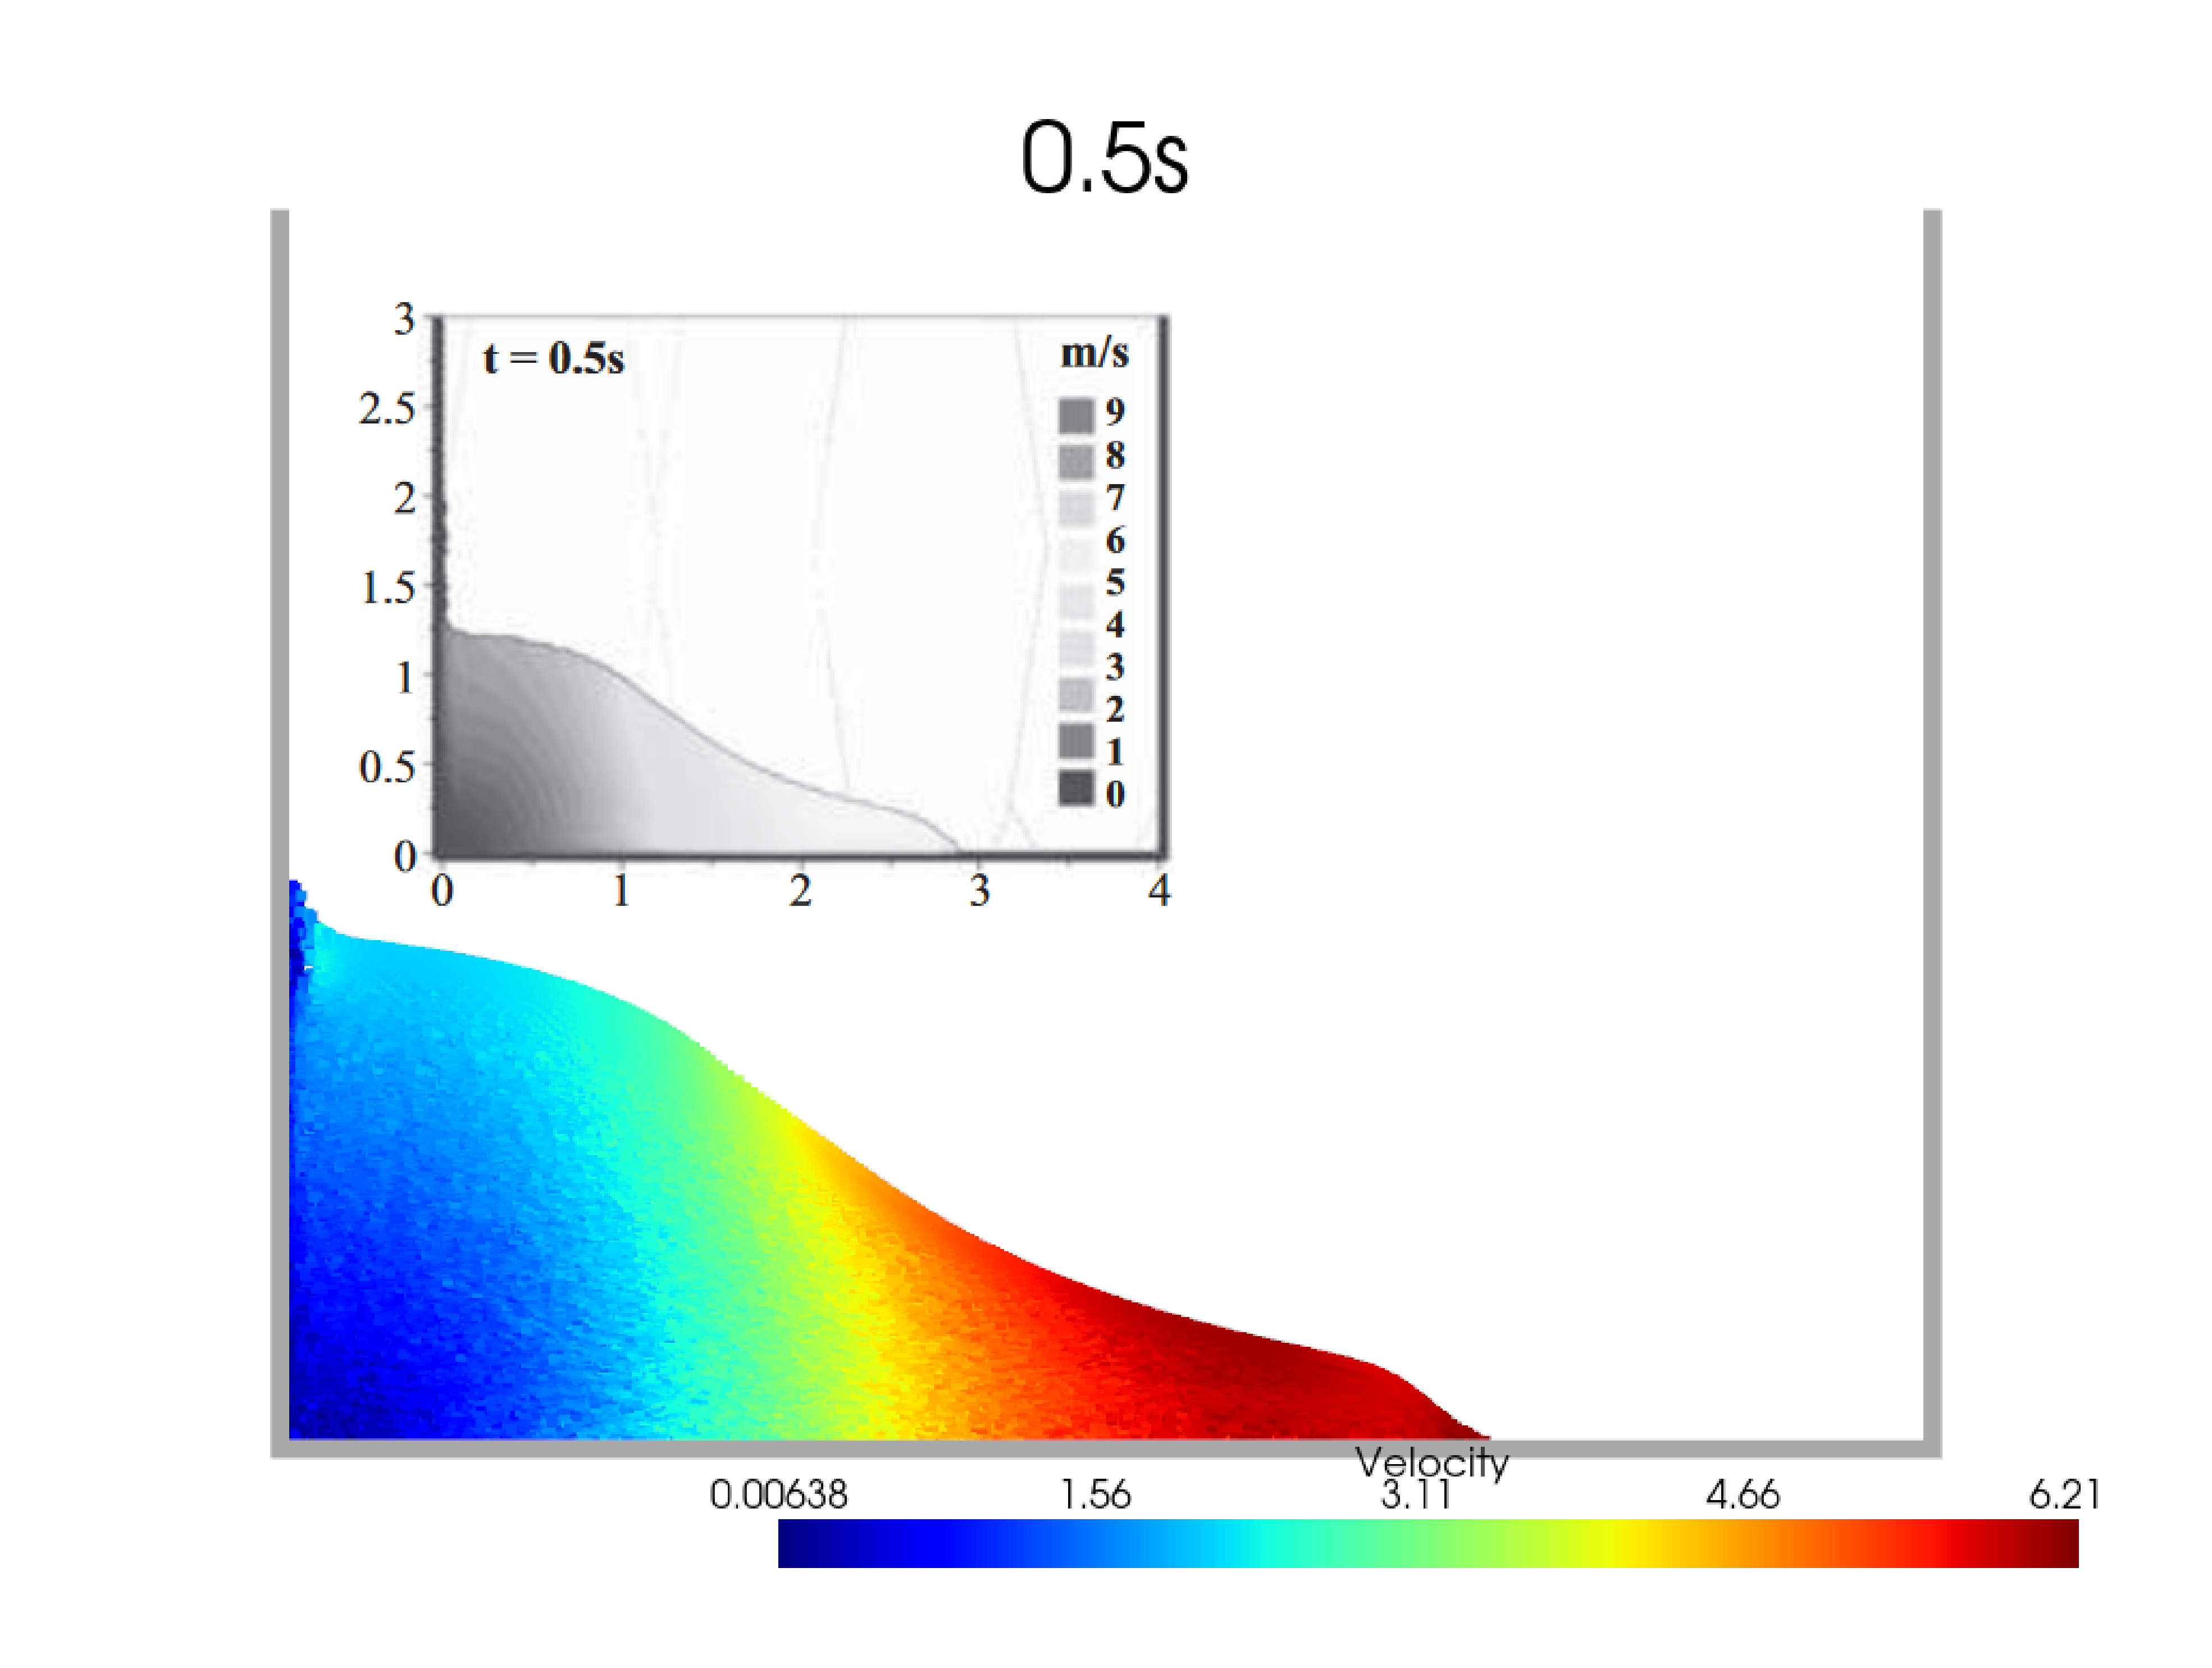
\includegraphics[width=0.47\textwidth]{images/CollapseDry/half/collapse_dry05_combined.png}
        }
    \end{figure}
\end{frame}

\begin{frame}
    \begin{figure}[H]
        \centering
        \subfigure[壁面粒子未垫高]{
            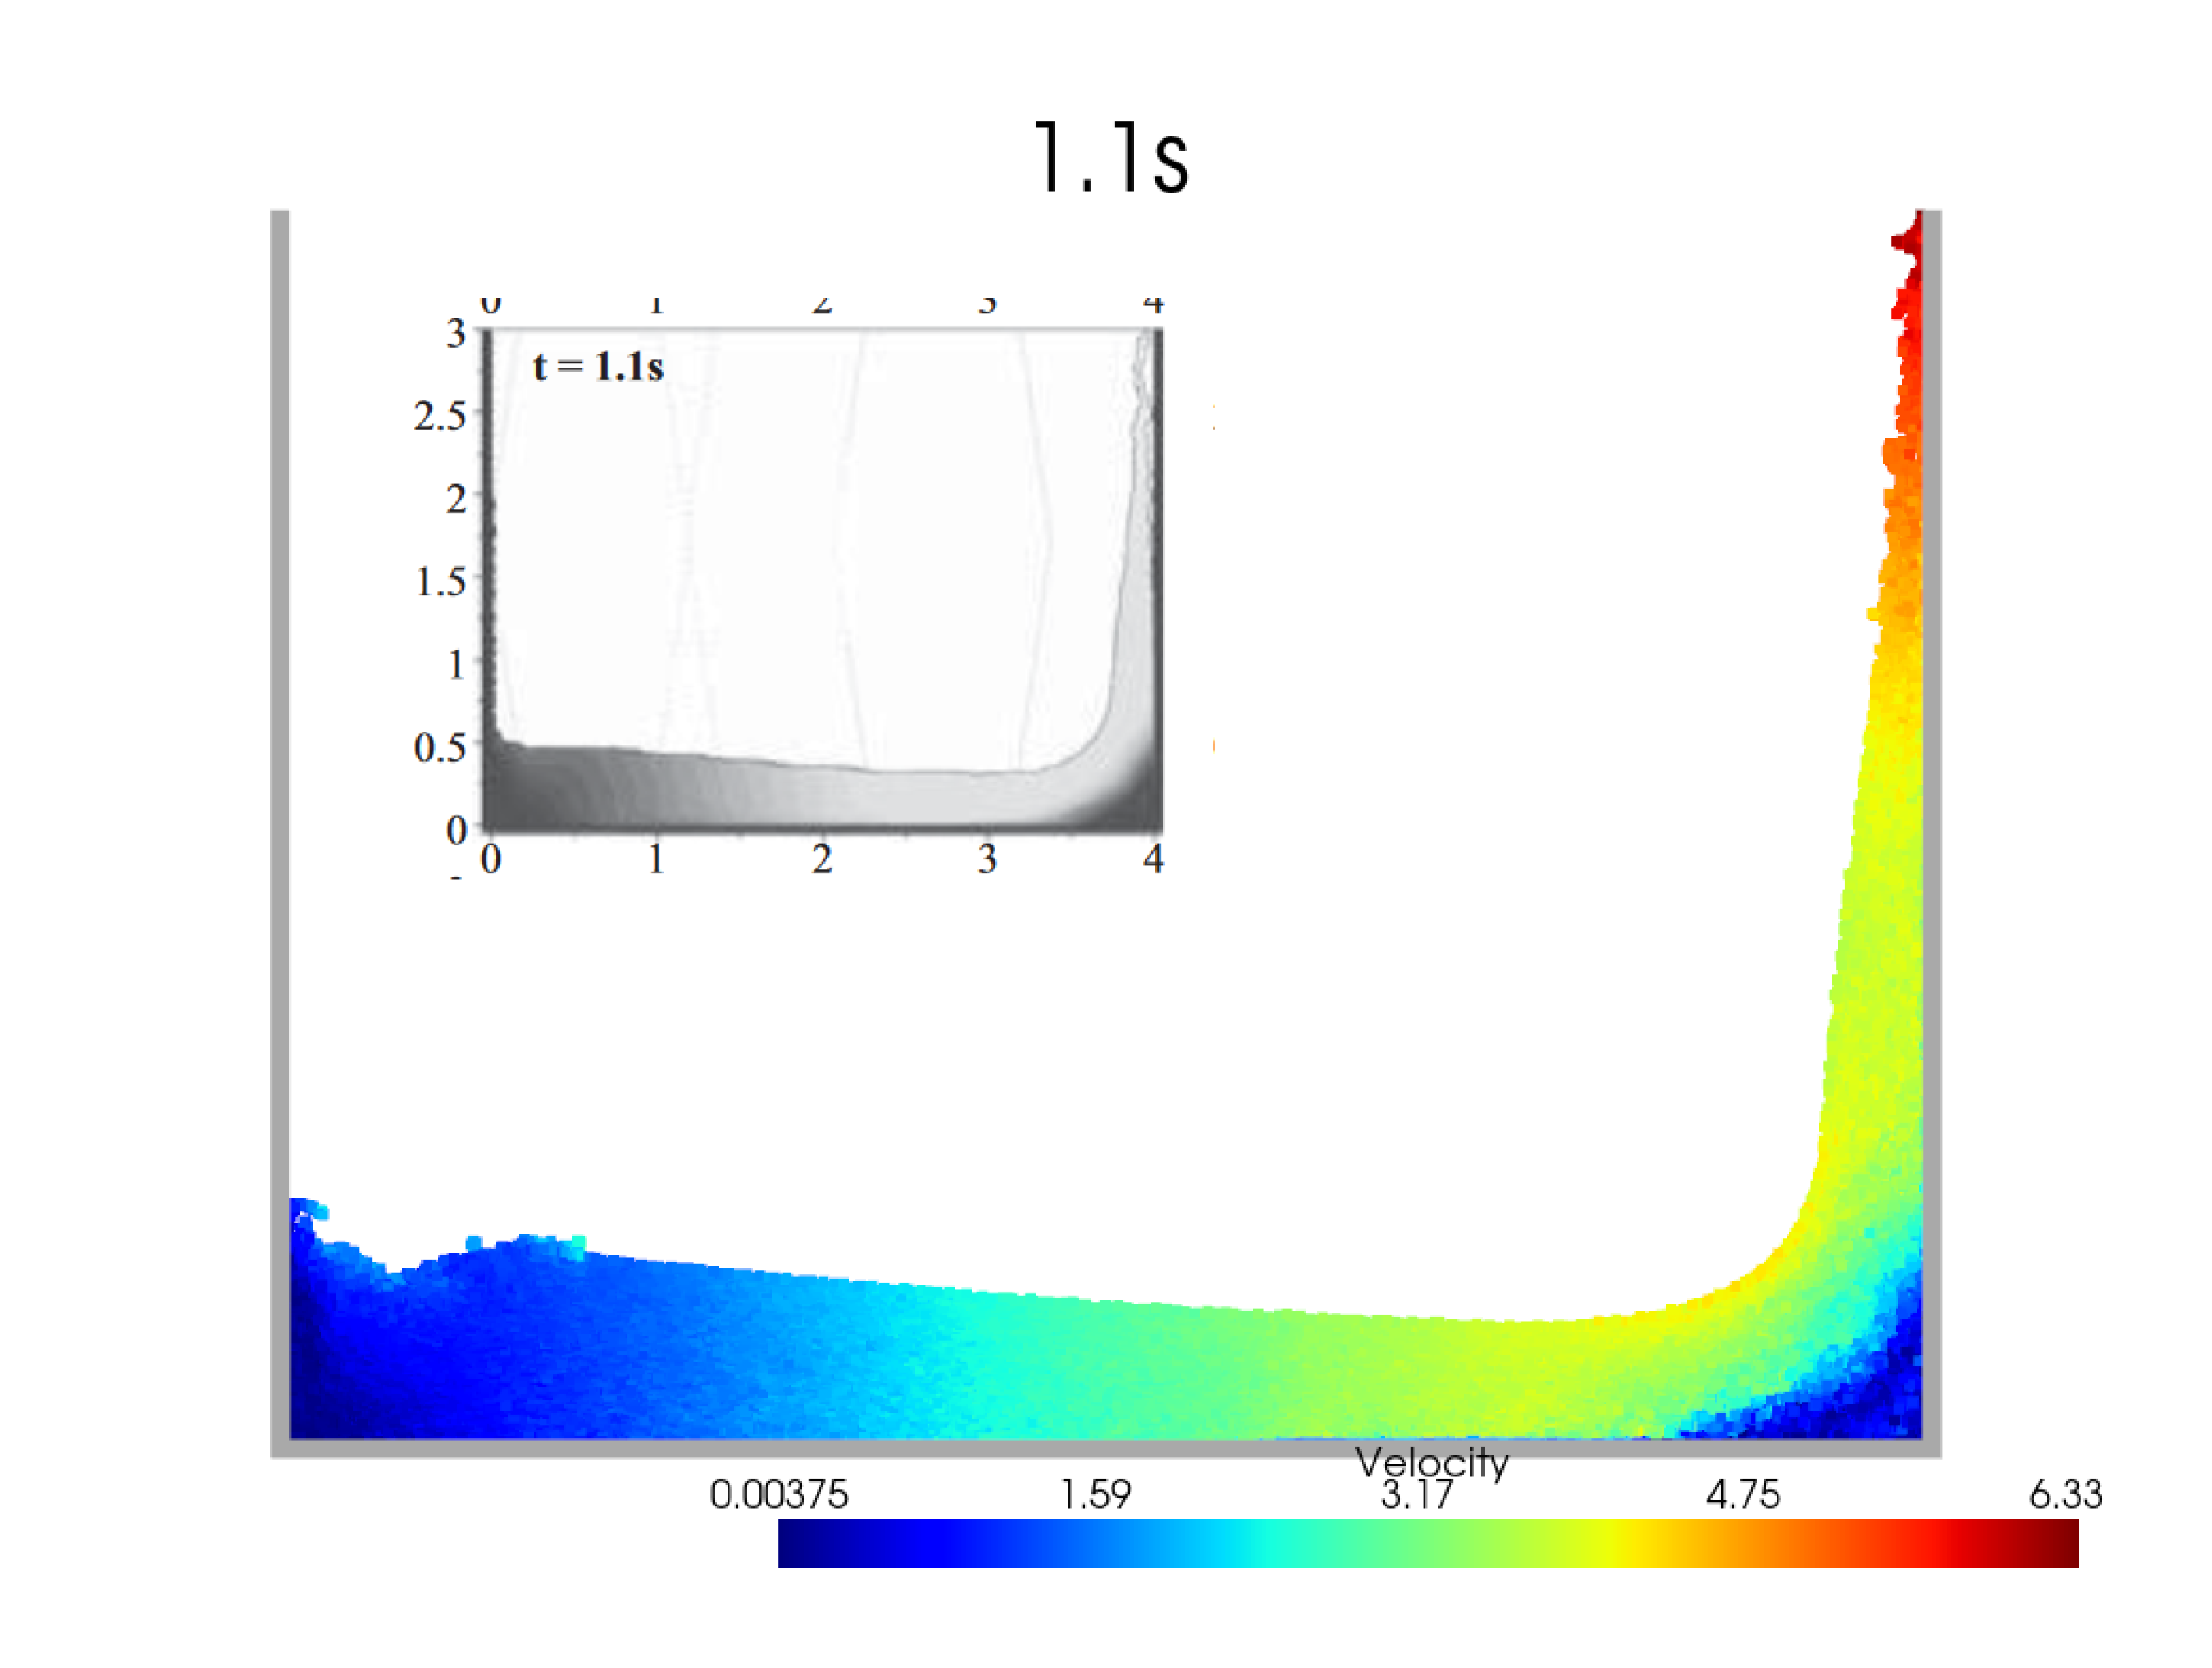
\includegraphics[width=0.47\textwidth]{images/CollapseDry/origin/collapse_dry11_combined.png}
        }
        \subfigure[壁面粒子垫高]{
            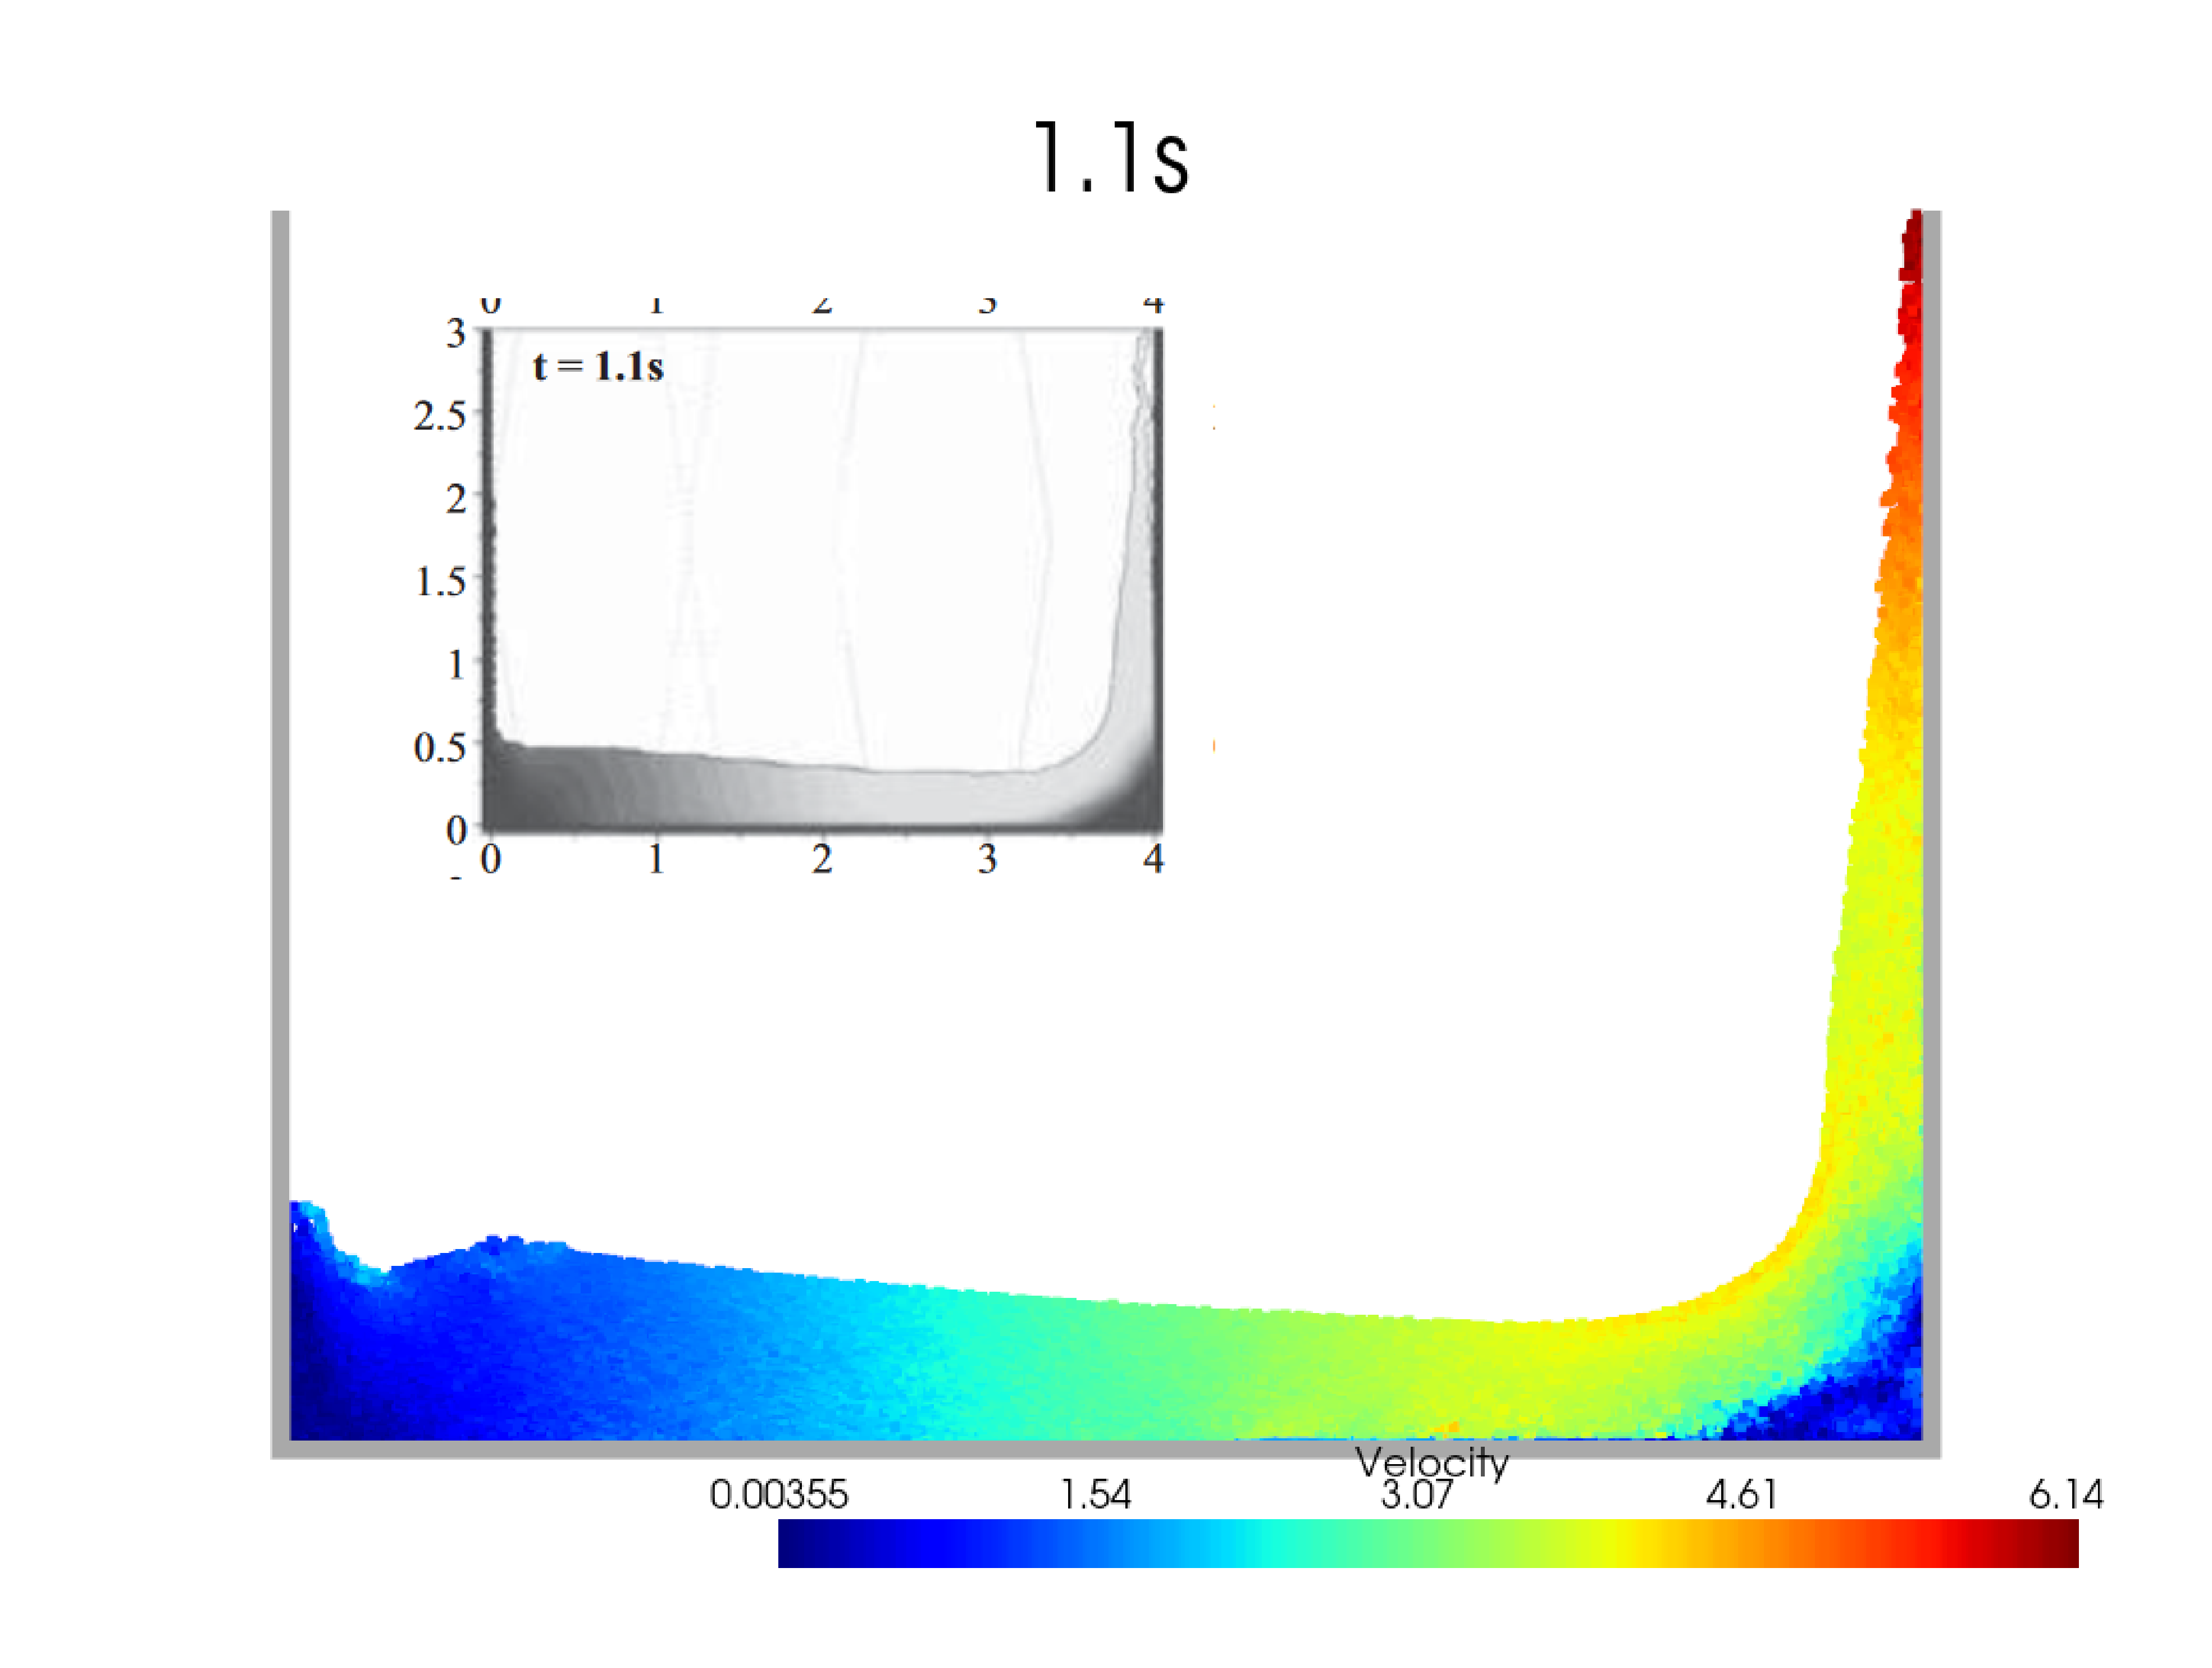
\includegraphics[width=0.47\textwidth]{images/CollapseDry/half/collapse_dry11_combined.png}
        }
    \end{figure}
\end{frame}

\begin{frame}
    \begin{figure}[H]
        \centering
        \subfigure[壁面粒子未垫高]{
            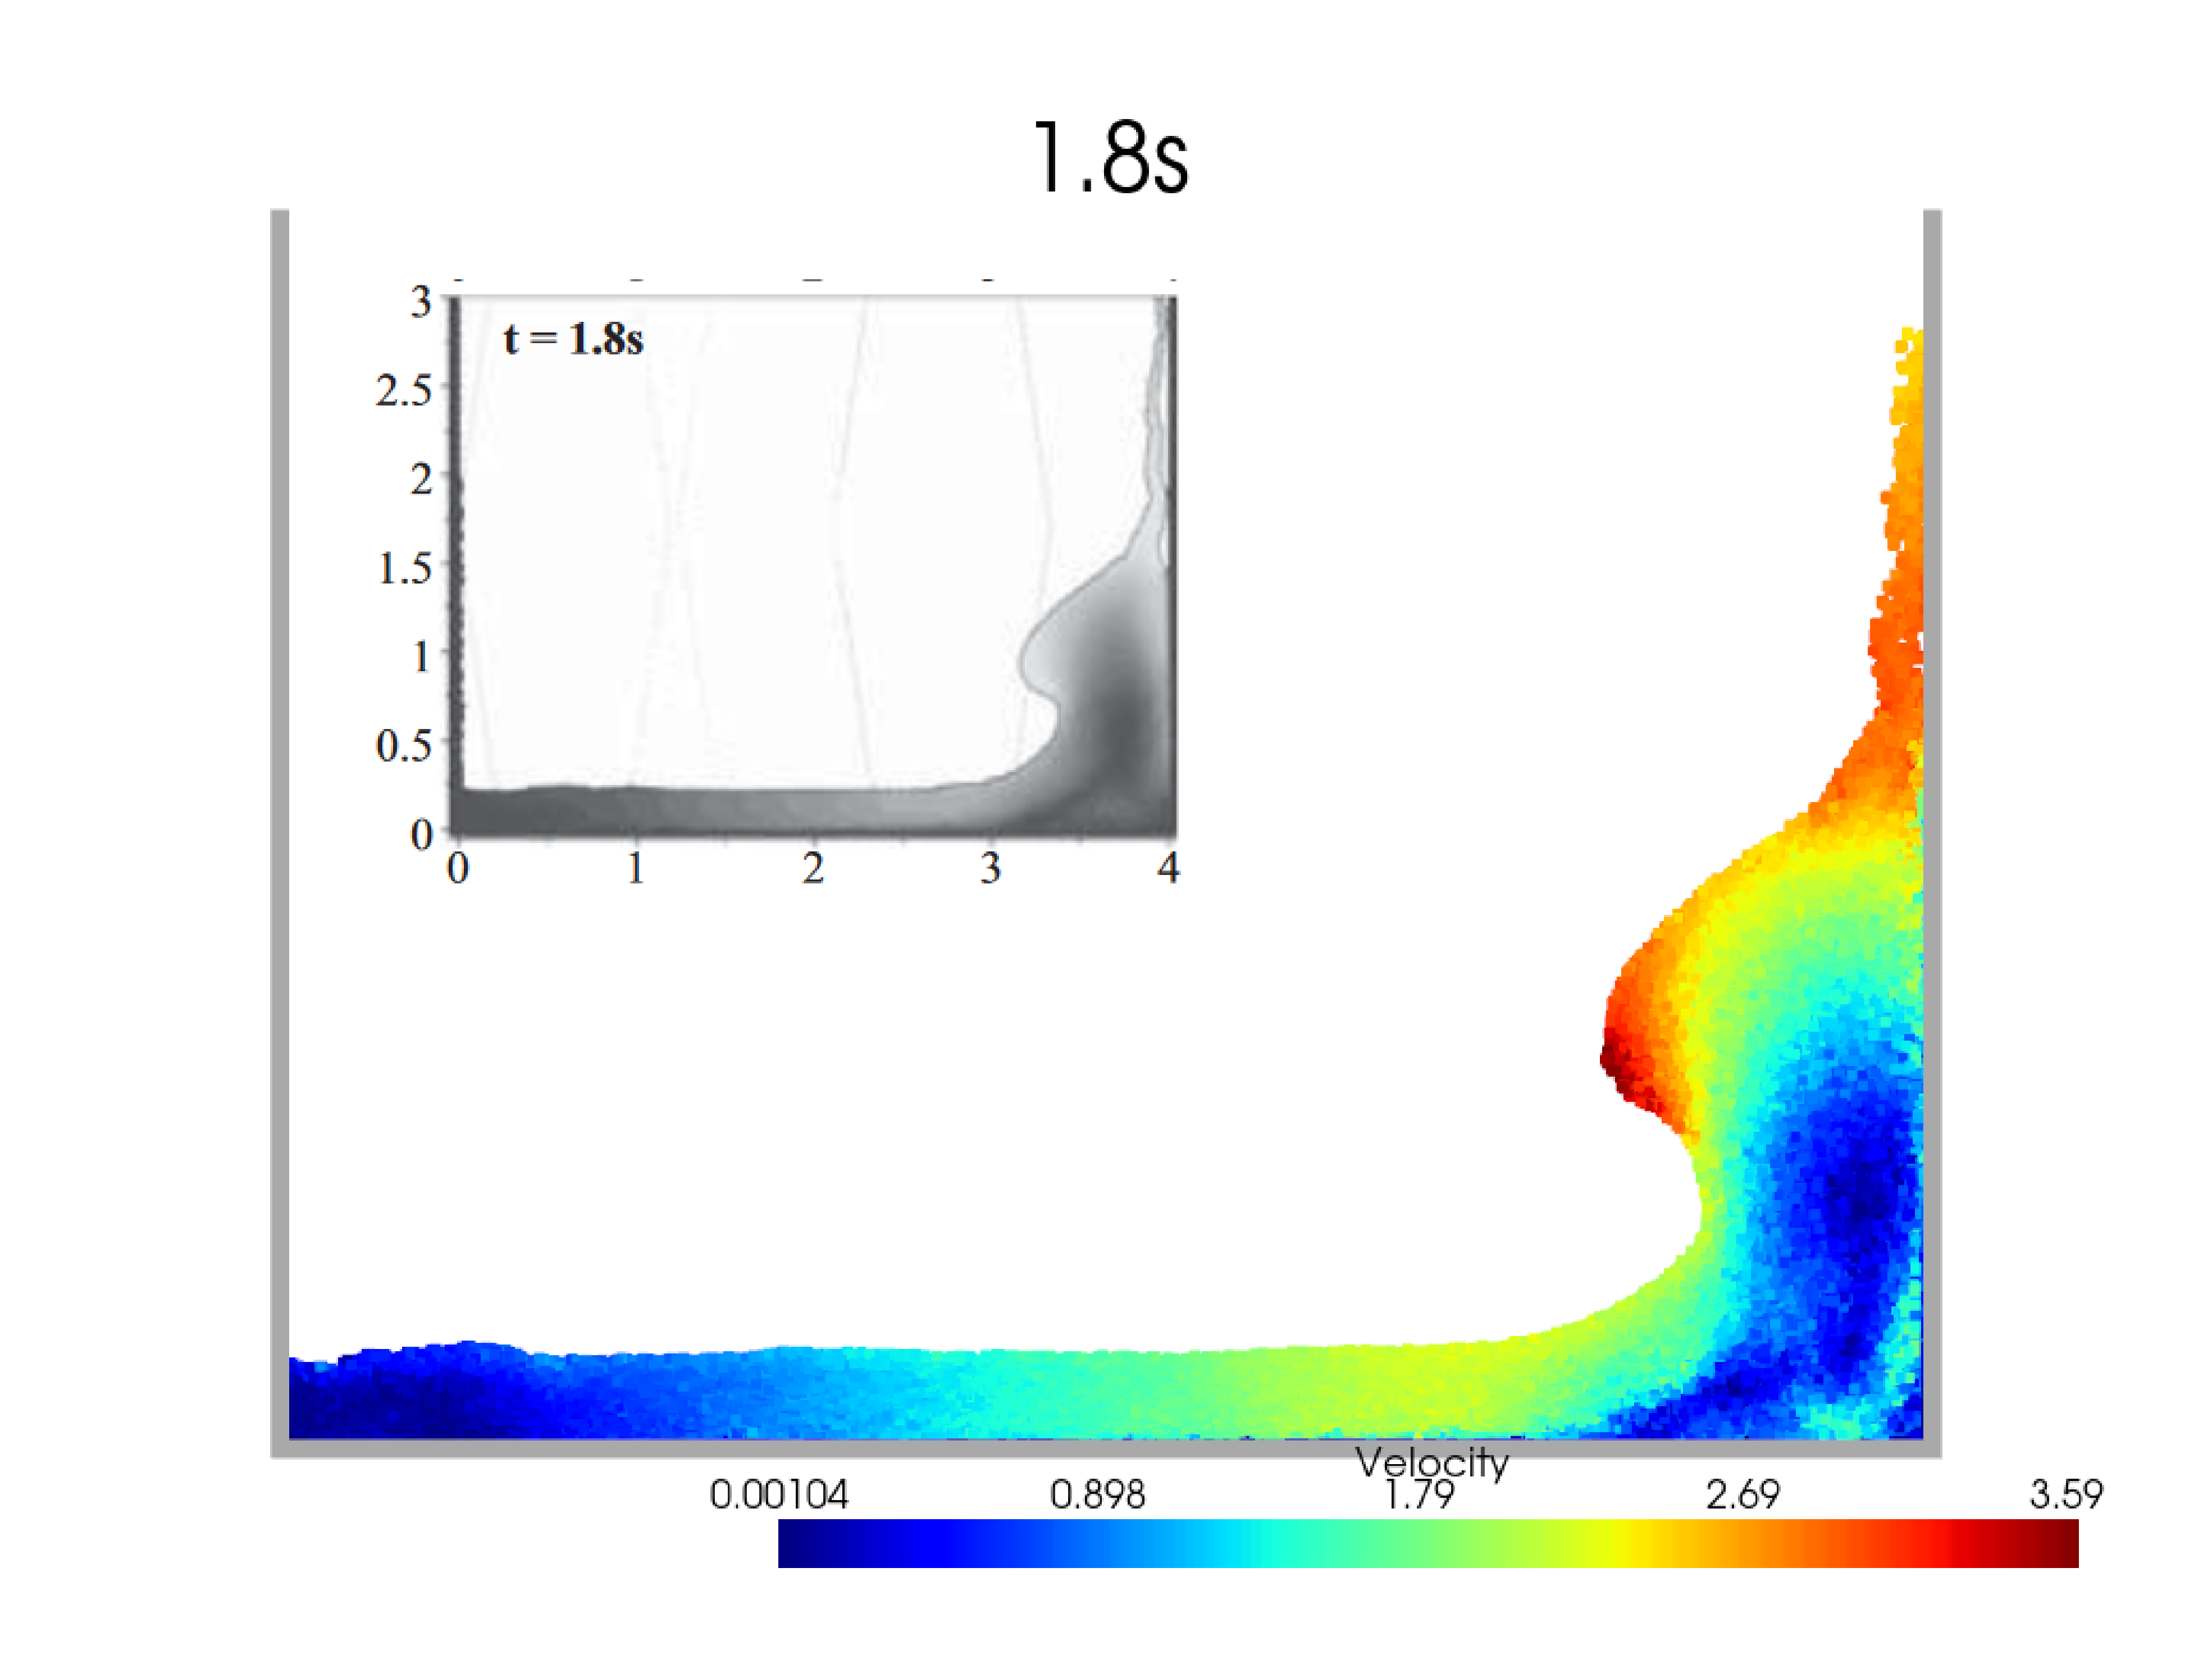
\includegraphics[width=0.47\textwidth]{images/CollapseDry/origin/collapse_dry18_combined.png}
        }
        \subfigure[壁面粒子垫高]{
            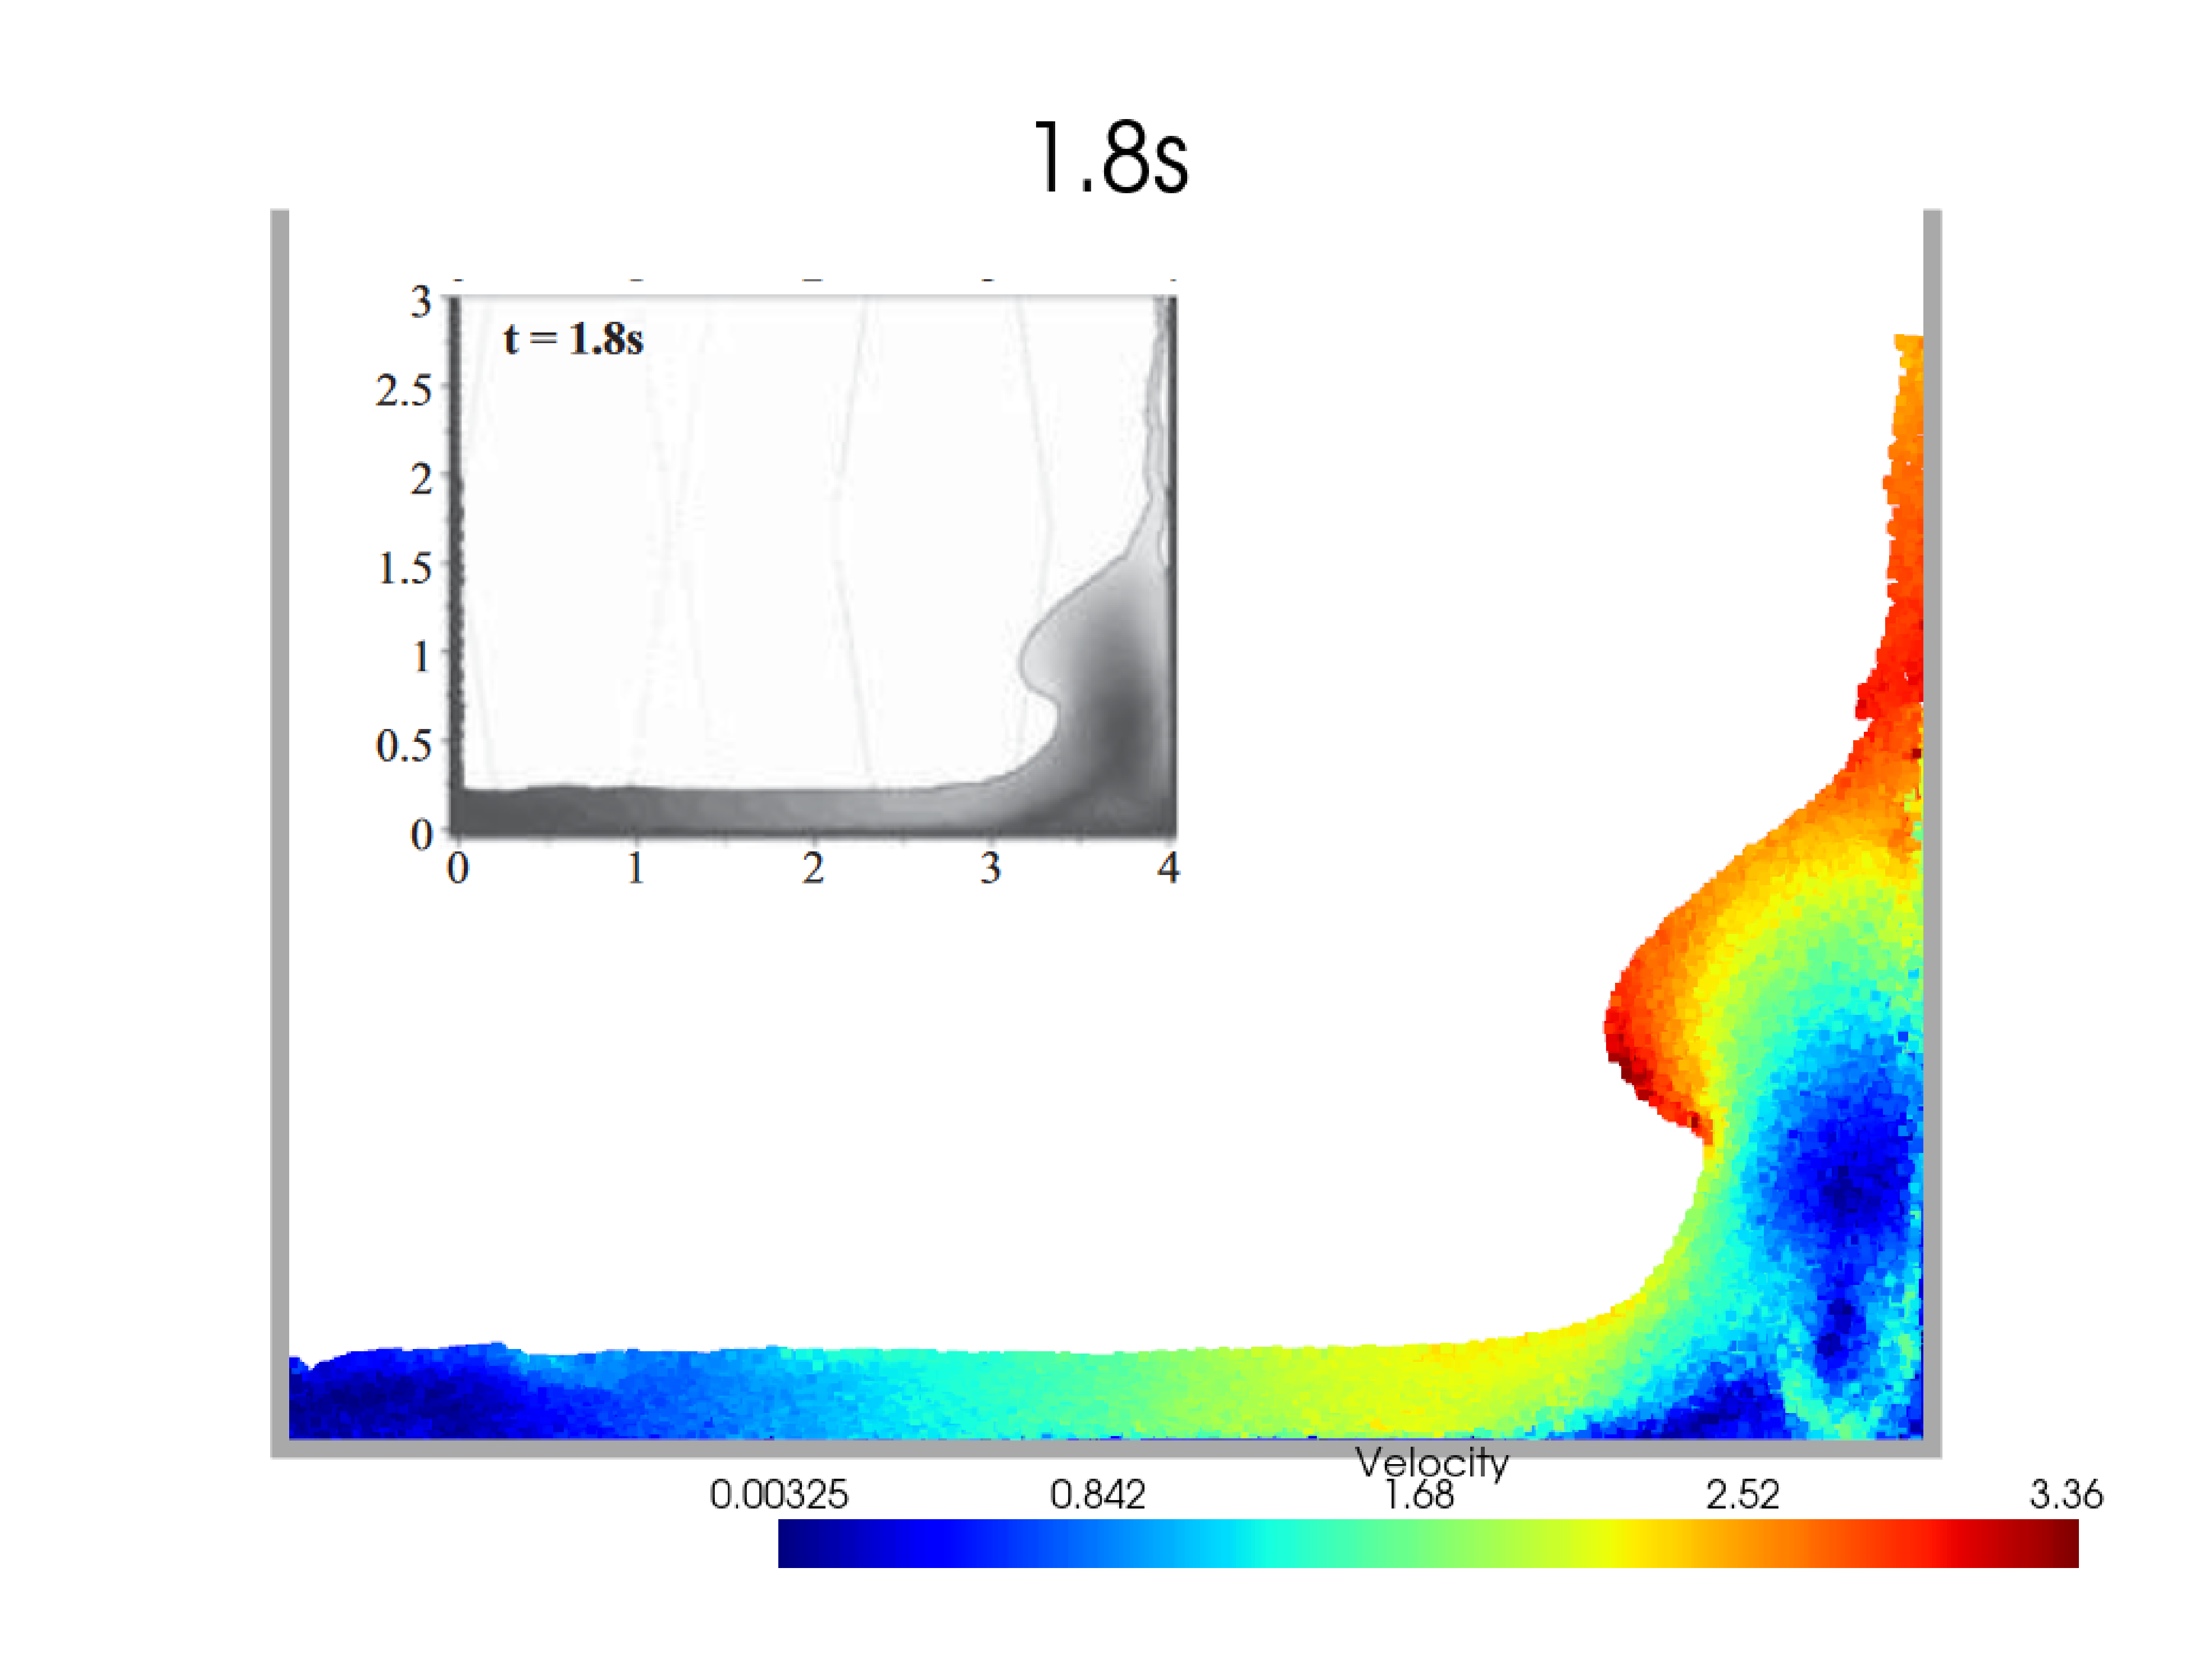
\includegraphics[width=0.47\textwidth]{images/CollapseDry/half/collapse_dry18_combined.png}
        }
    \end{figure}
\end{frame}

\begin{frame}
    \begin{figure}[H]
        \centering
        \subfigure[壁面粒子未垫高]{
            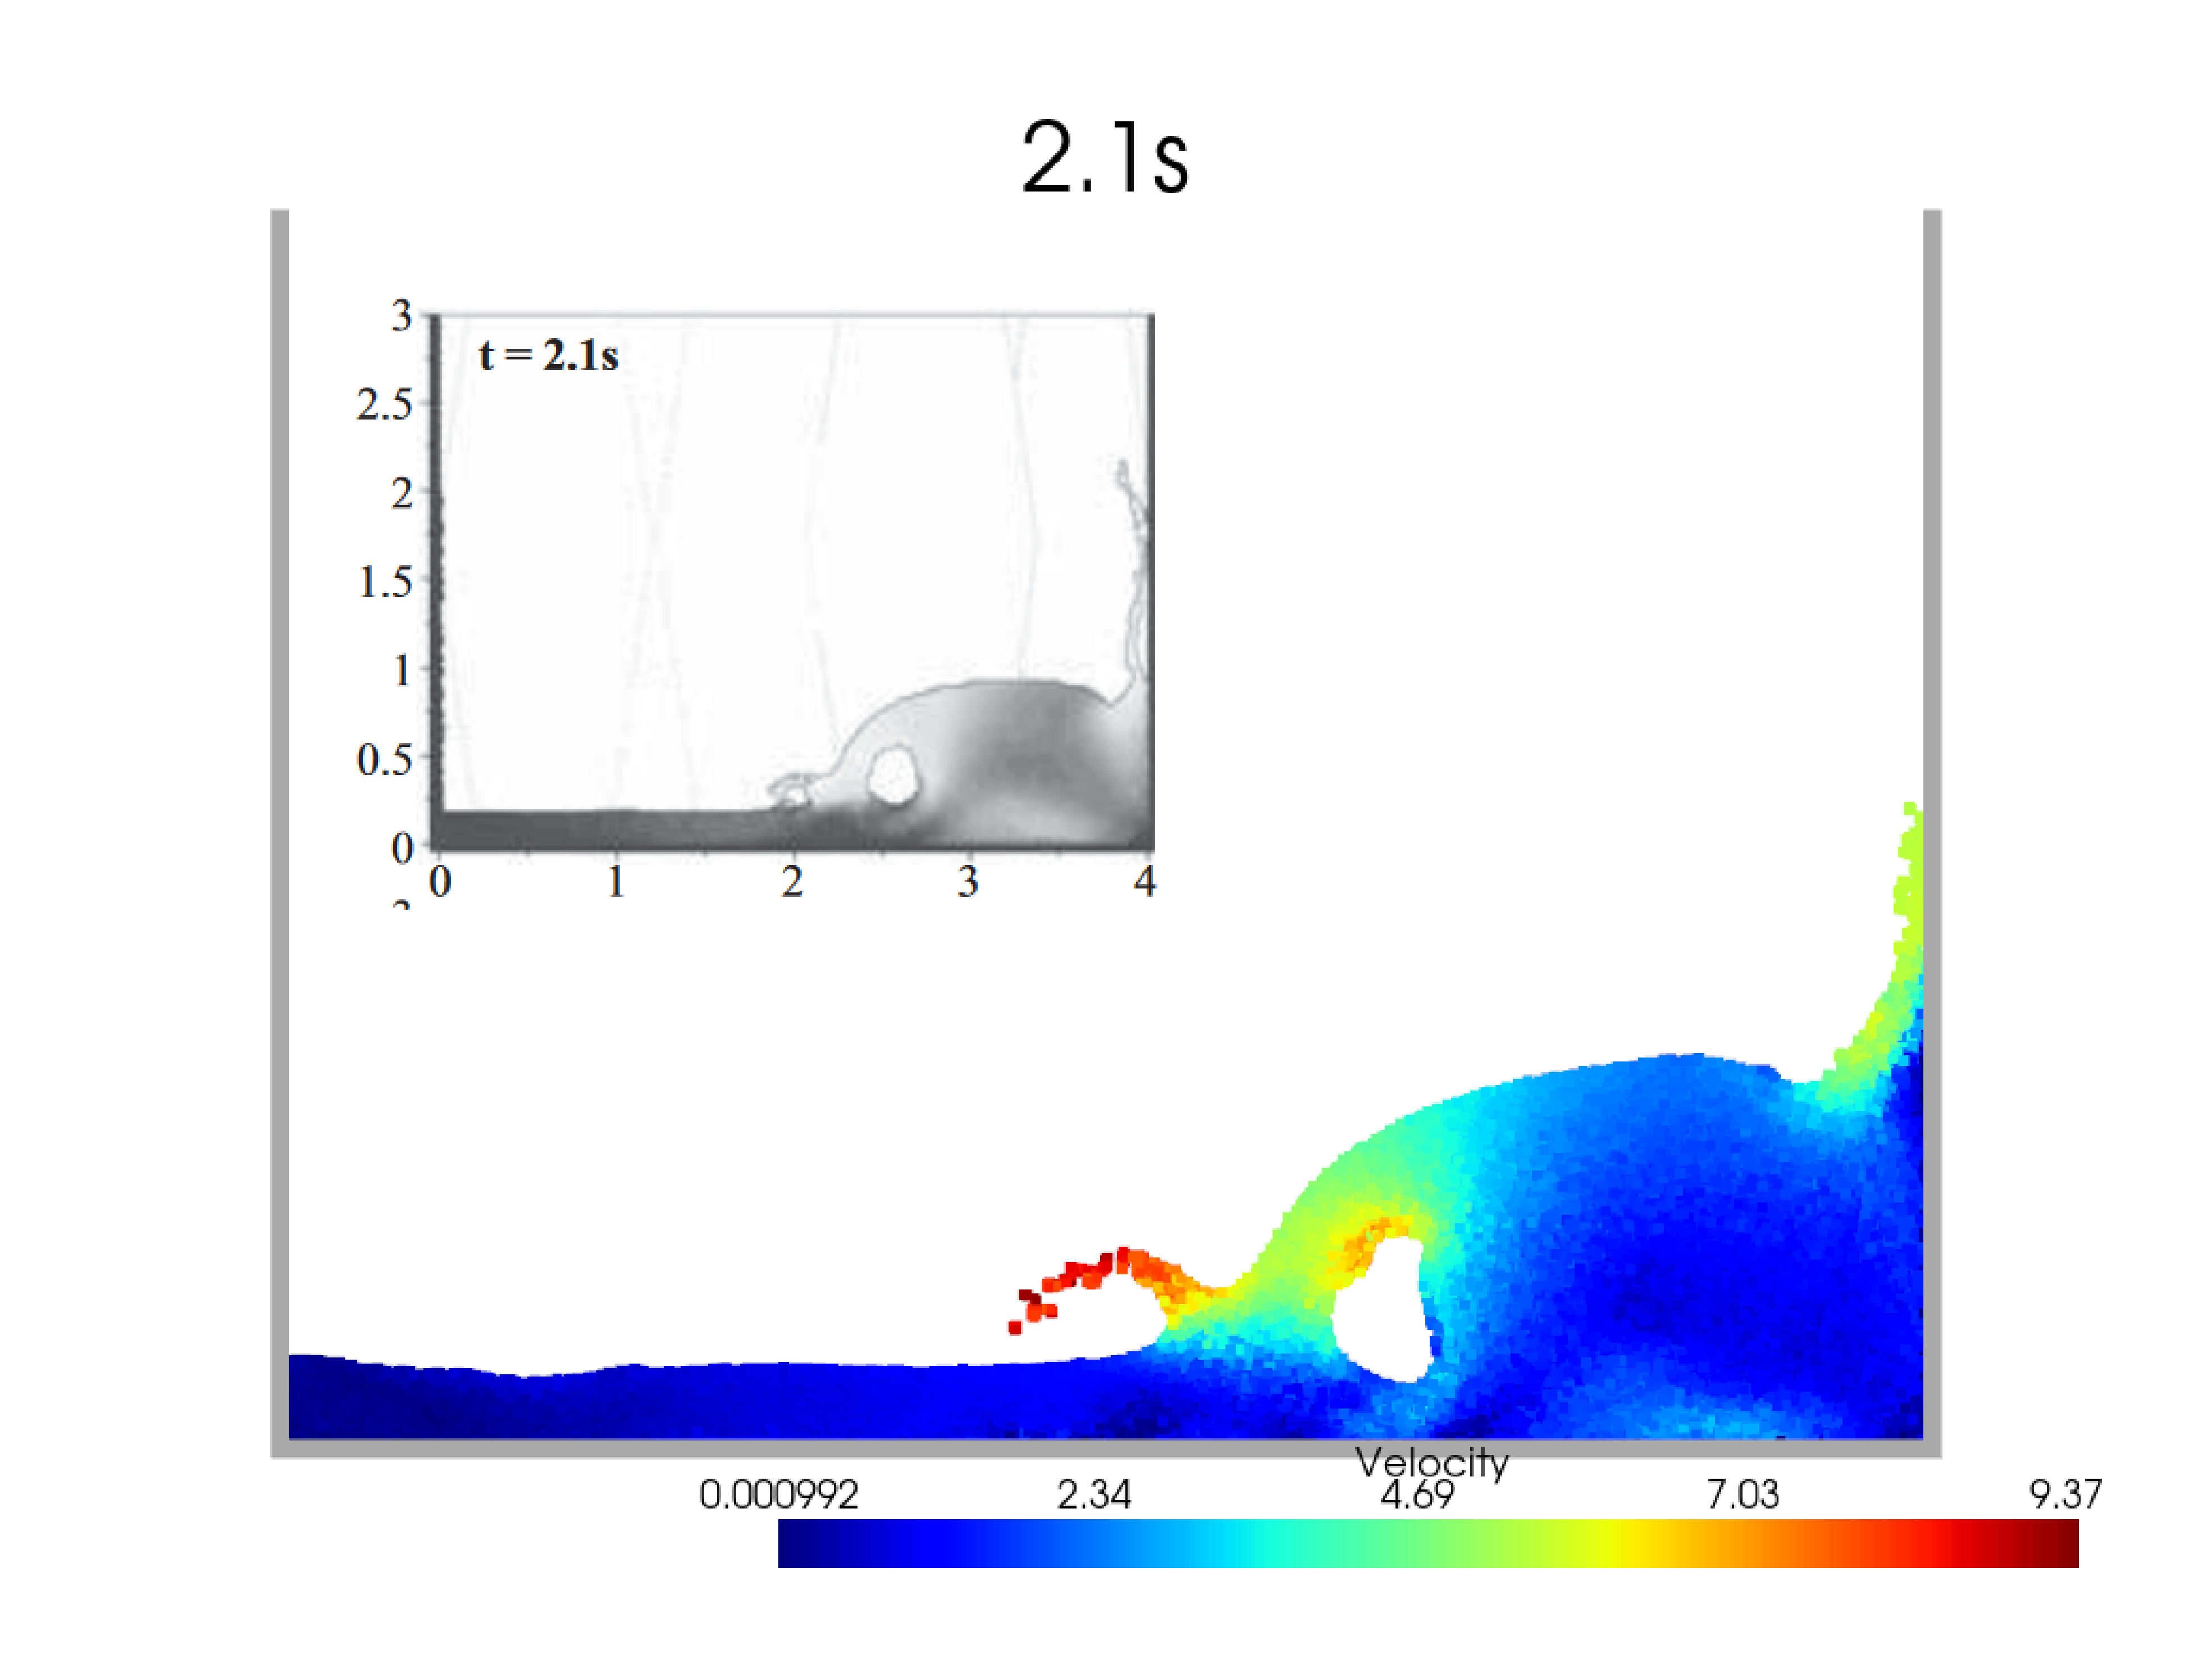
\includegraphics[width=0.47\textwidth]{images/CollapseDry/origin/collapse_dry21_combined.png}
        }
        \subfigure[壁面粒子垫高]{
            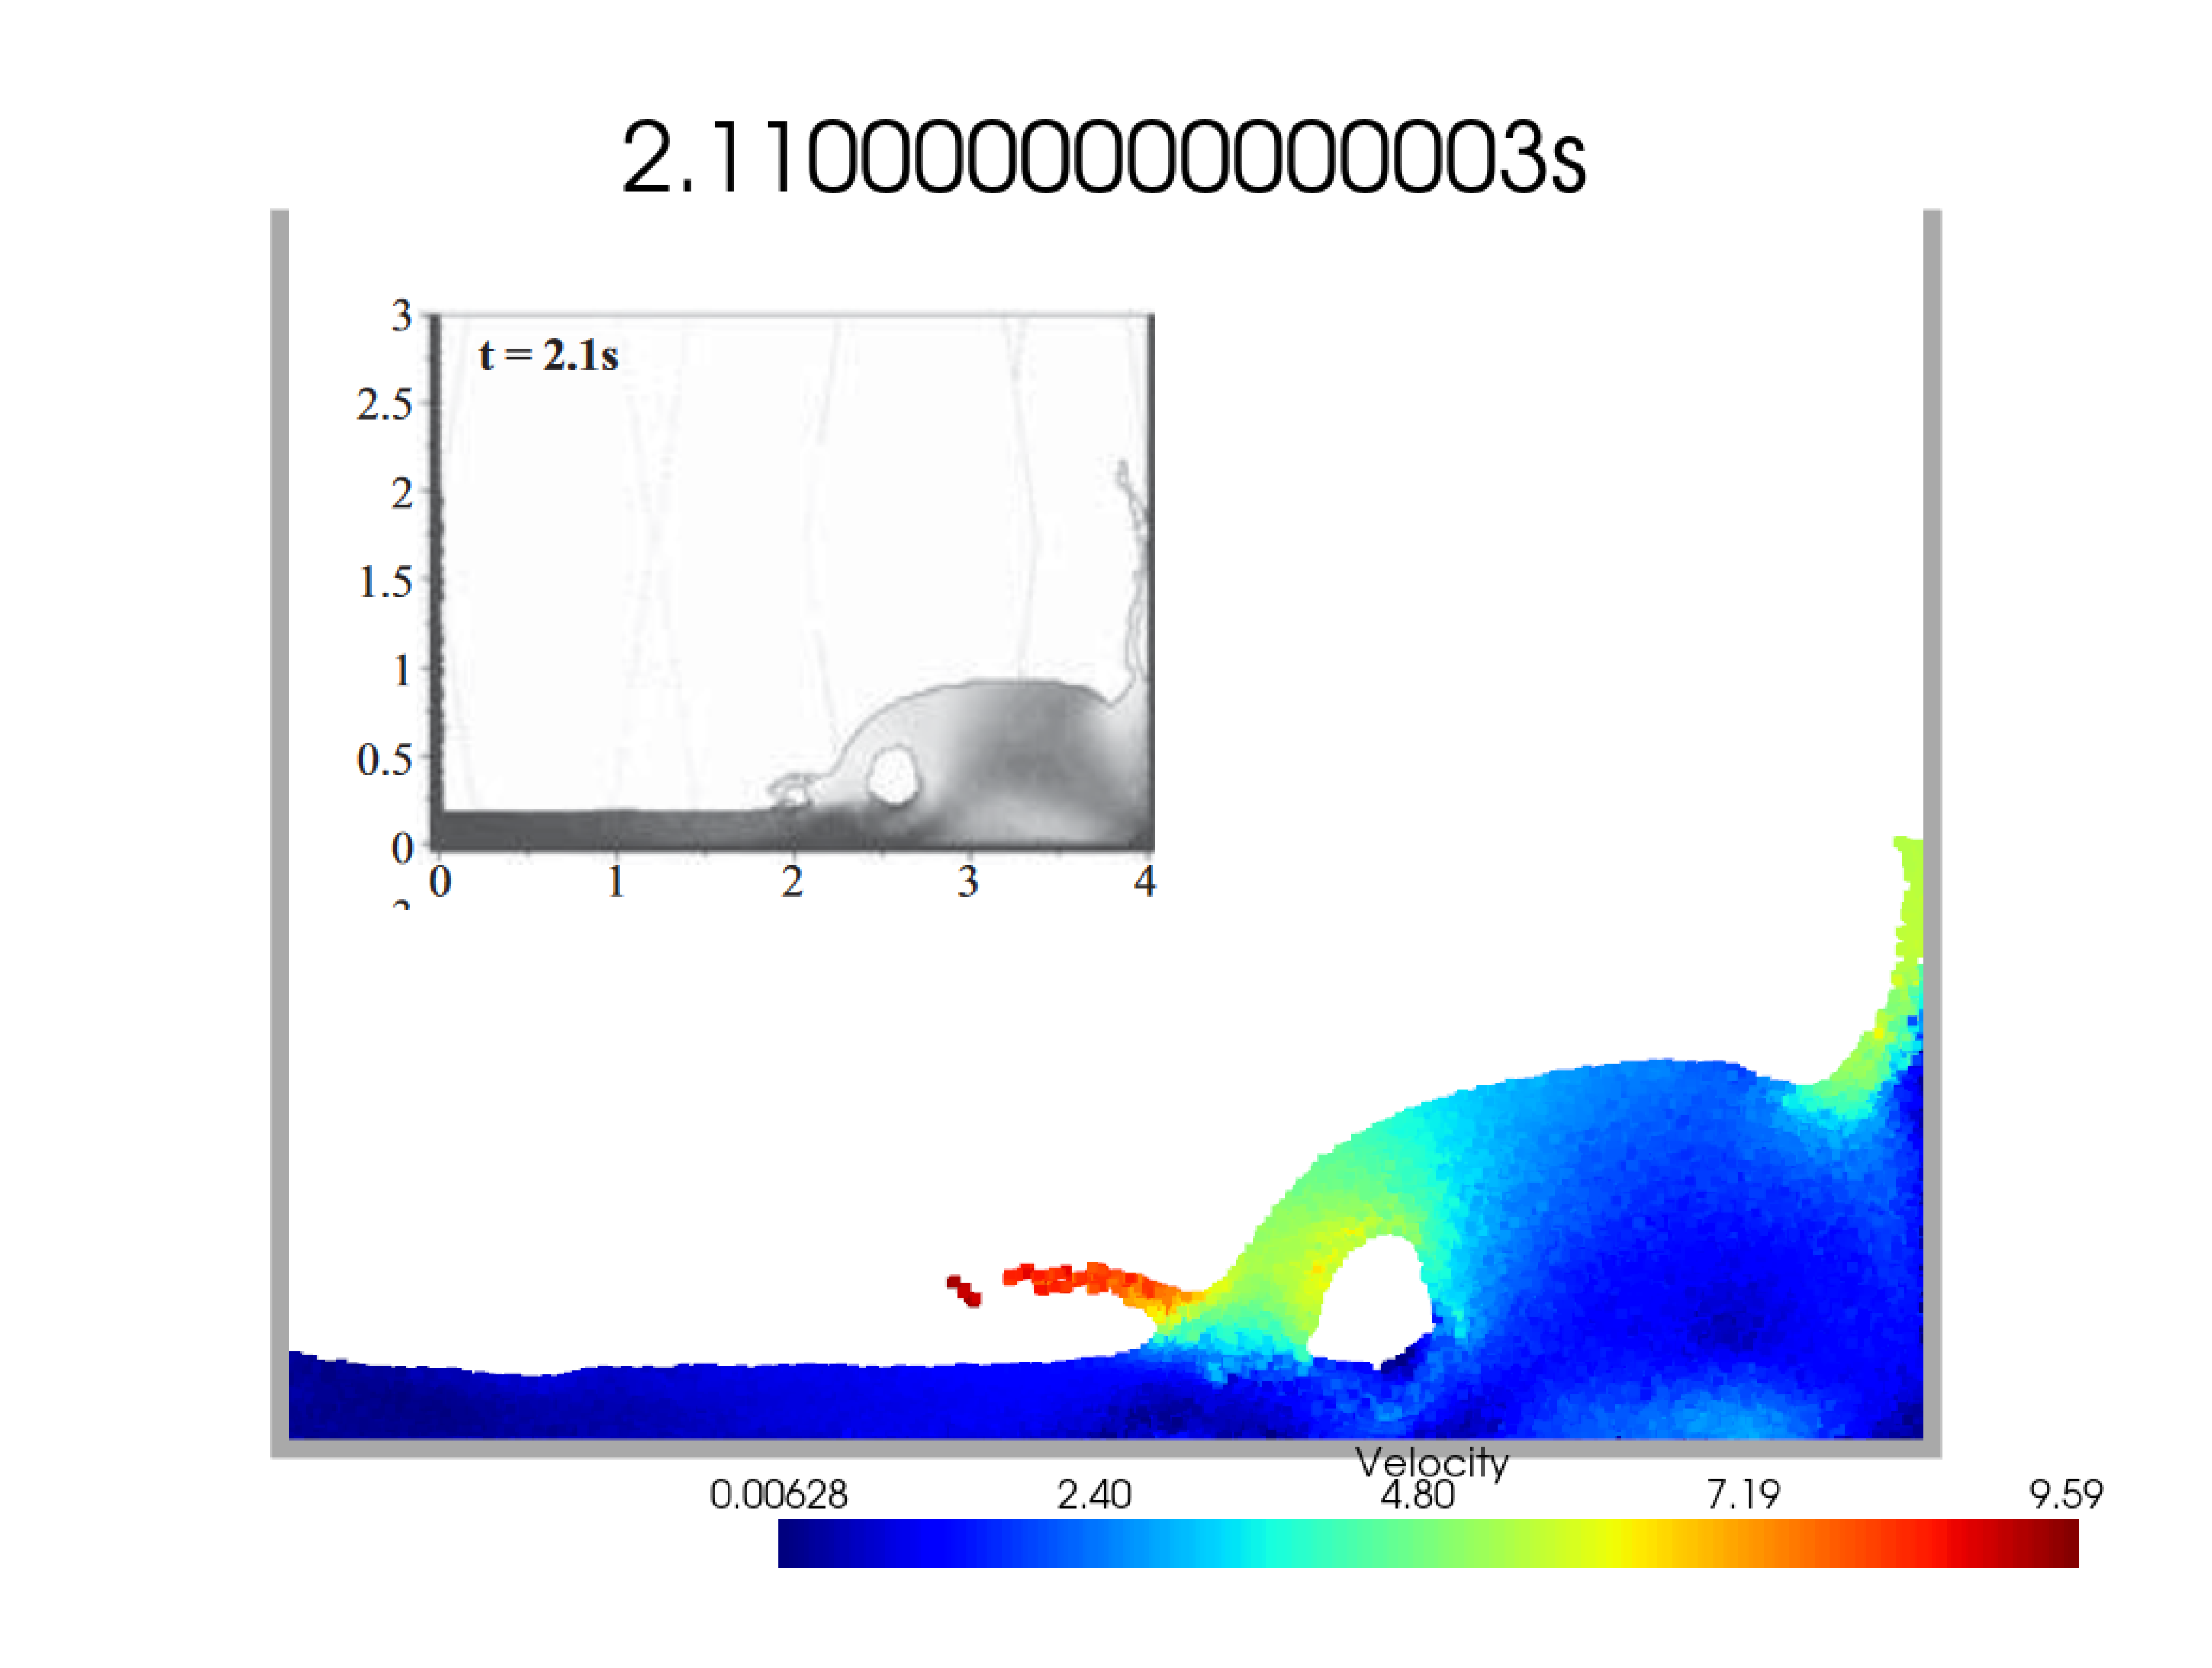
\includegraphics[width=0.47\textwidth]{images/CollapseDry/half/collapse_dry21_combined.png}
        }
    \end{figure}
\end{frame}

\begin{frame}
    \begin{figure}[H]
        \centering
        \subfigure[壁面粒子未垫高]{
            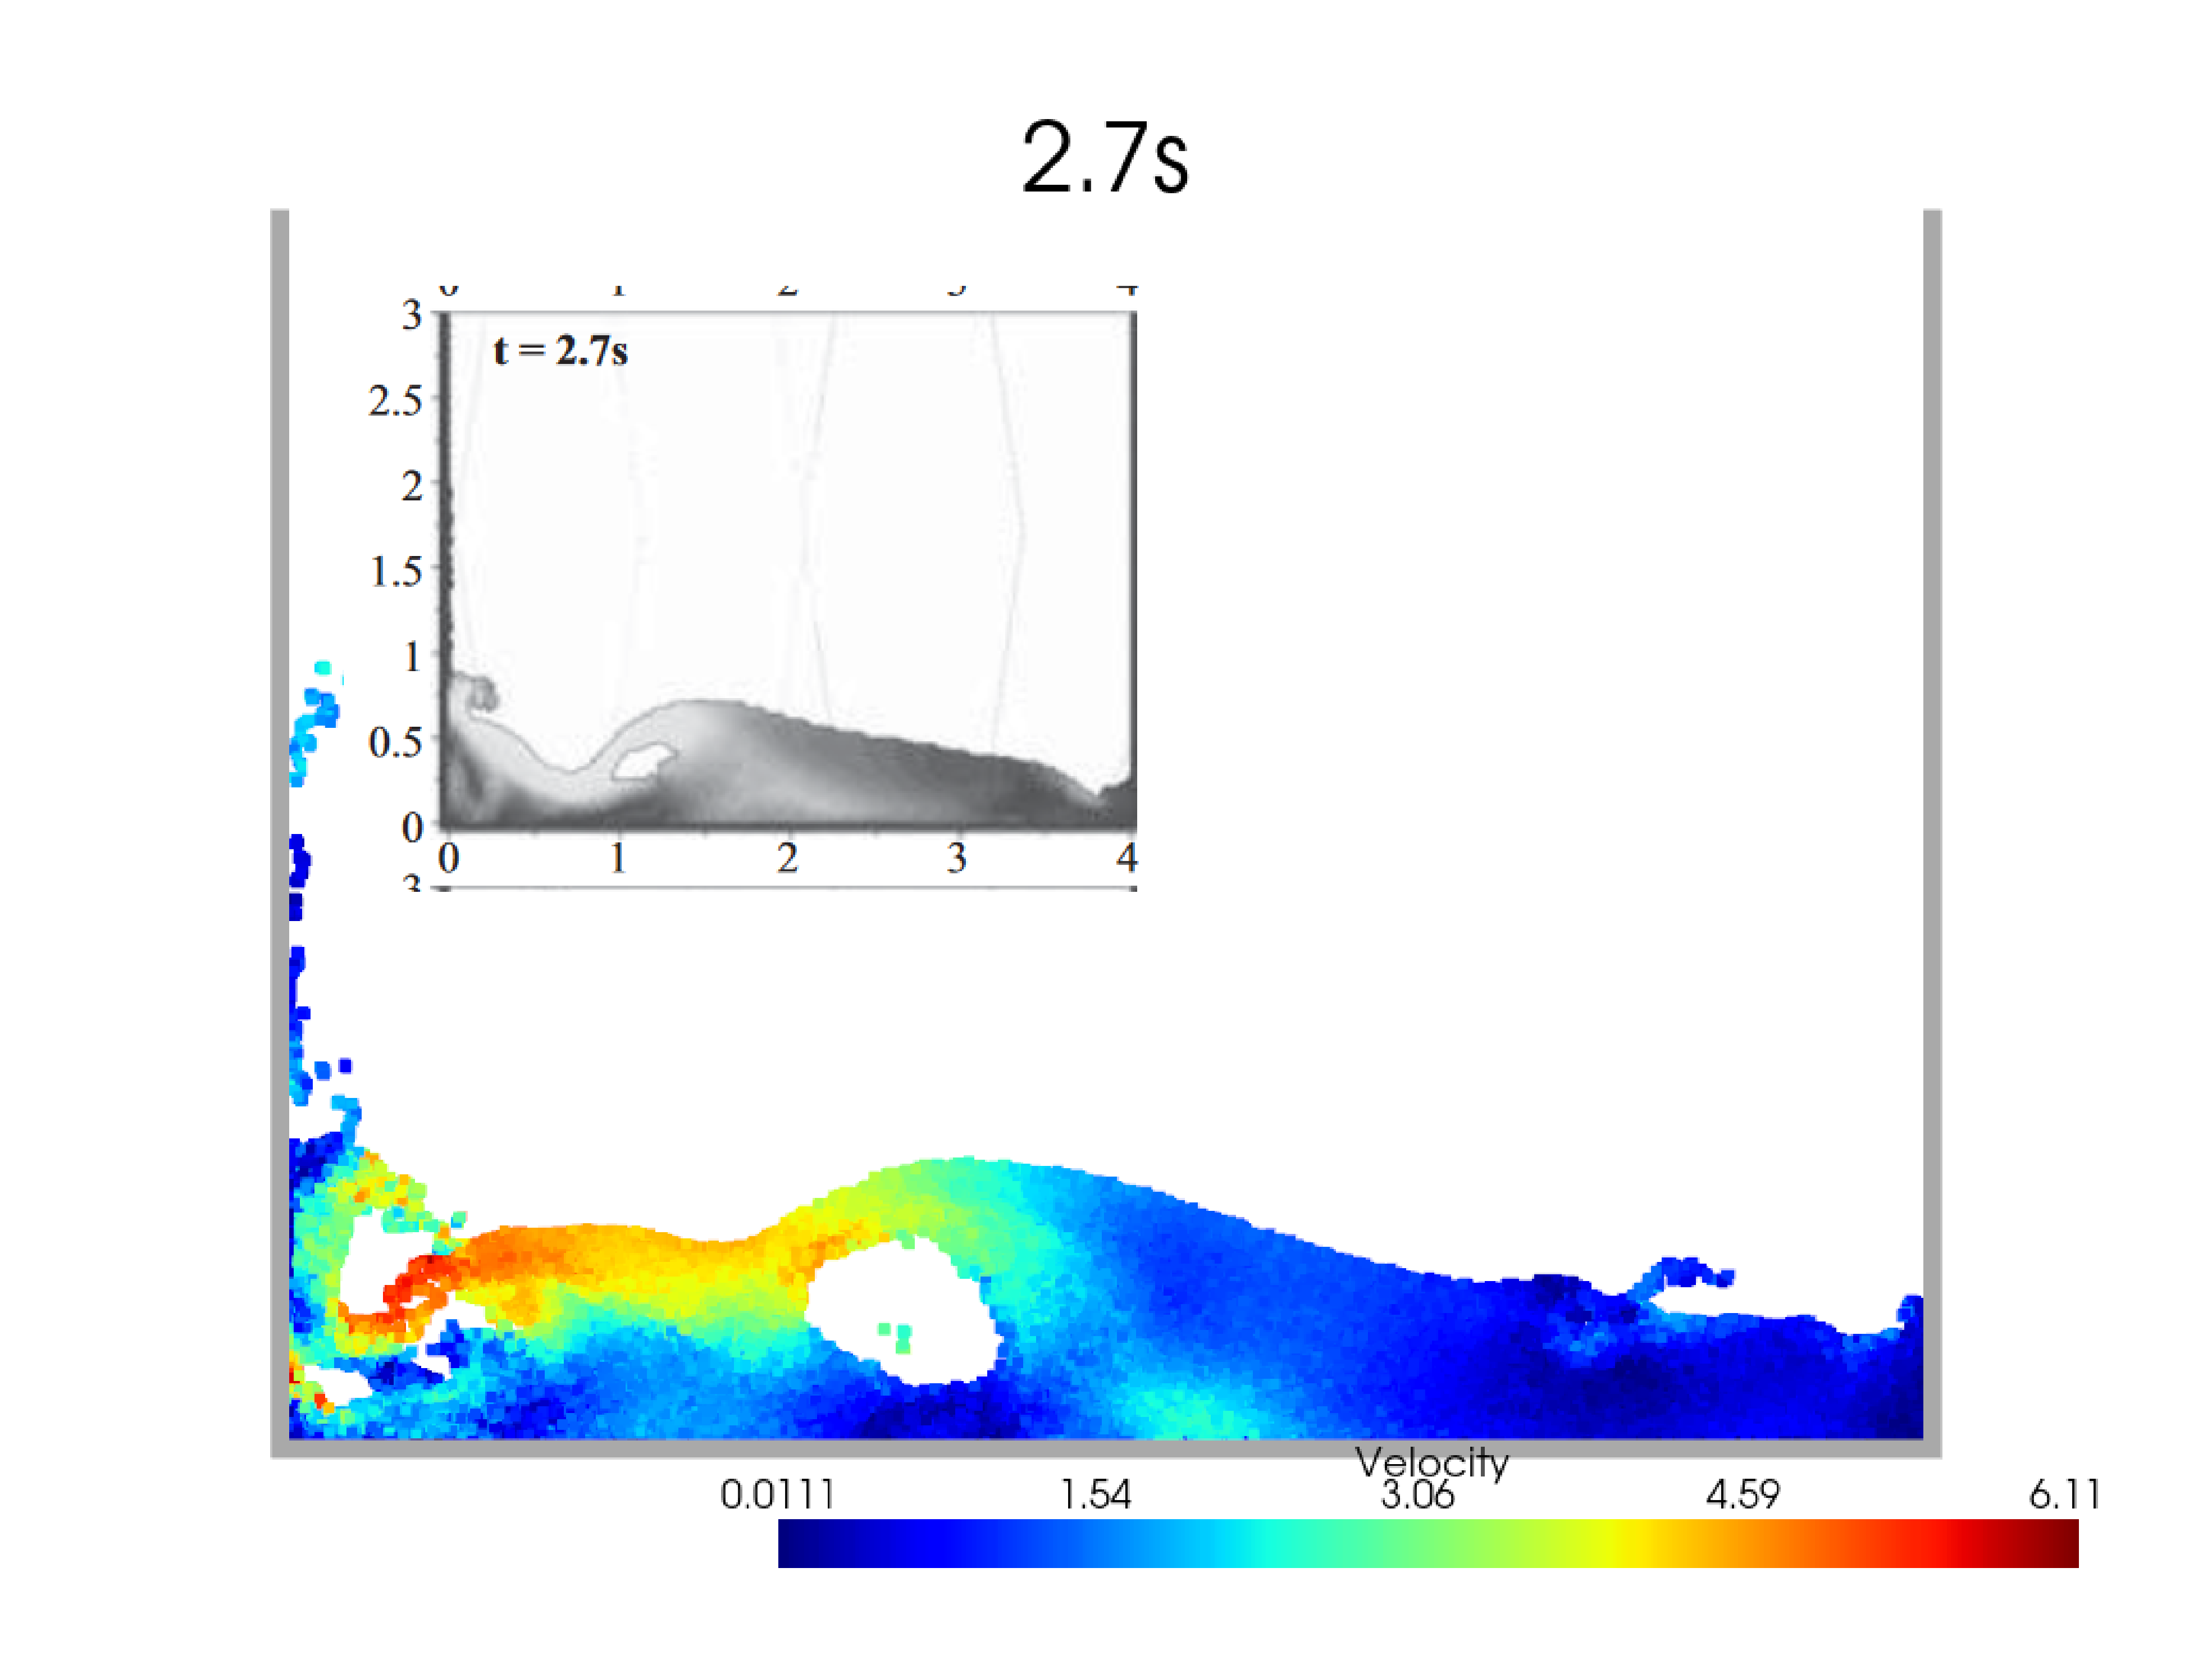
\includegraphics[width=0.47\textwidth]{images/CollapseDry/origin/collapse_dry27_combined.png}
        }
        \subfigure[壁面粒子垫高]{
            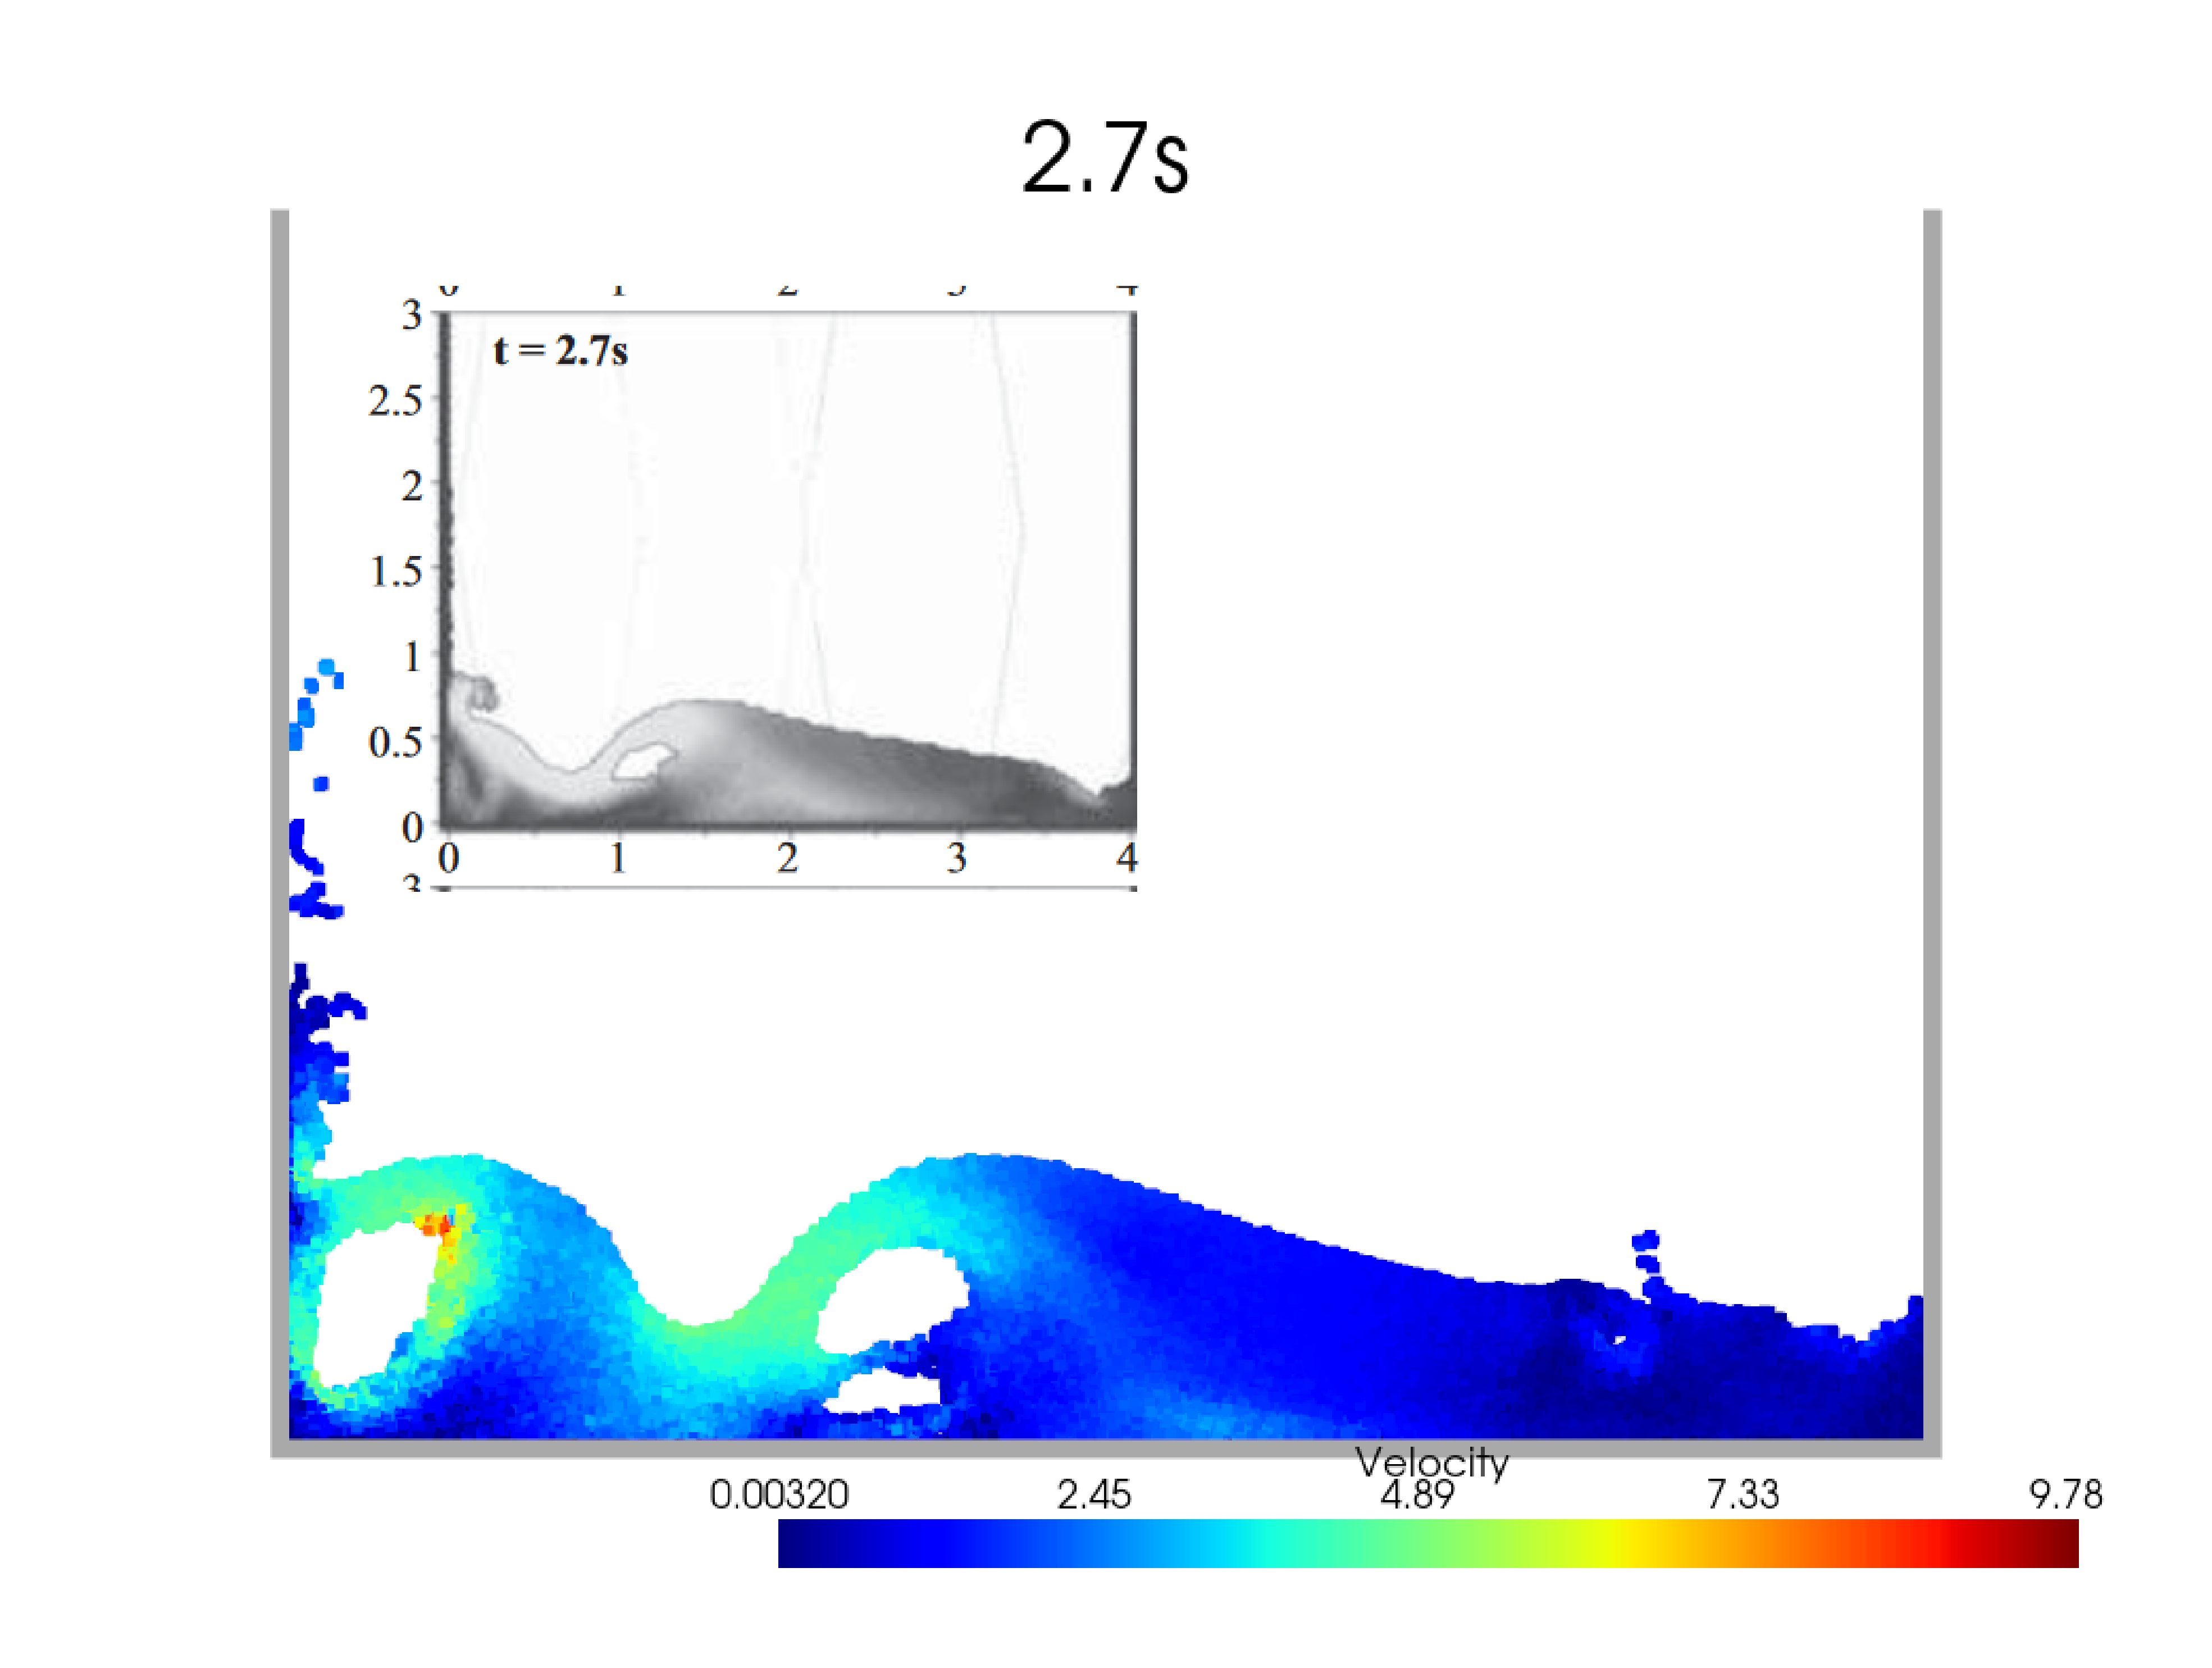
\includegraphics[width=0.47\textwidth]{images/CollapseDry/half/collapse_dry27_combined.png}
        }
    \end{figure}
\end{frame}

\begin{frame}
    \begin{figure}[H]
        \centering
        \subfigure[壁面粒子未垫高]{
            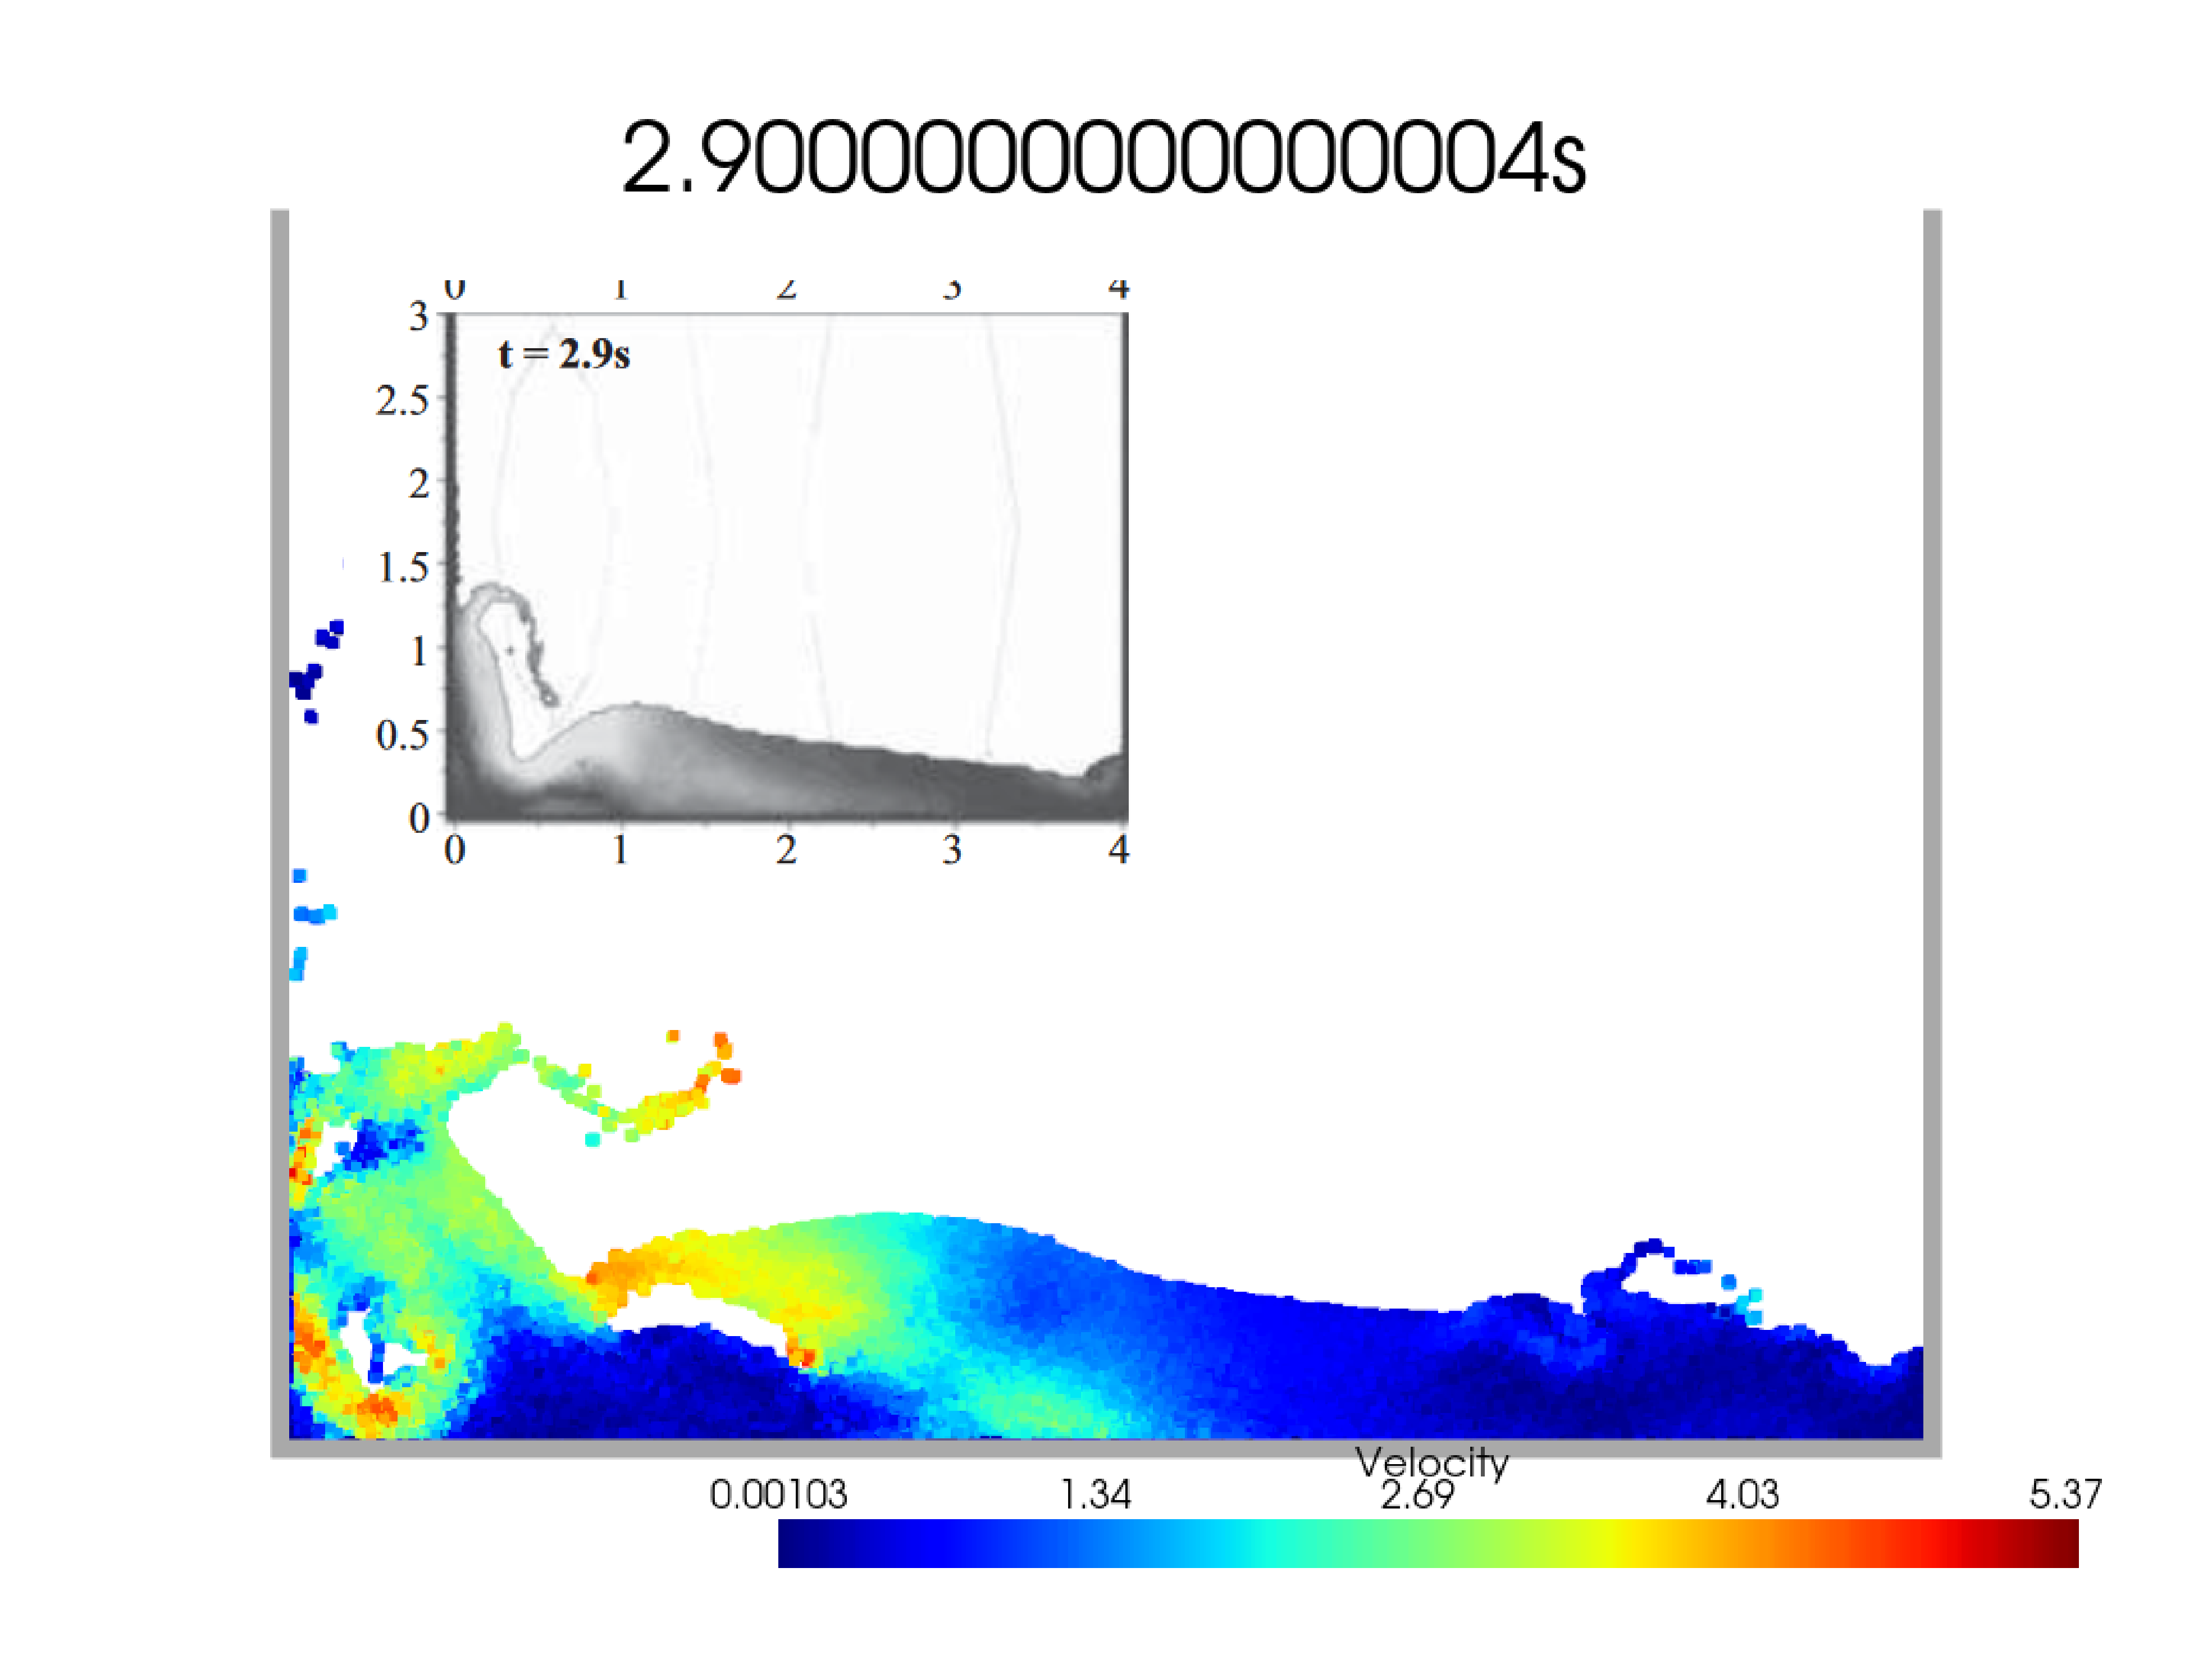
\includegraphics[width=0.47\textwidth]{images/CollapseDry/origin/collapse_dry29_combined.png}
        }
        \subfigure[壁面粒子垫高]{
            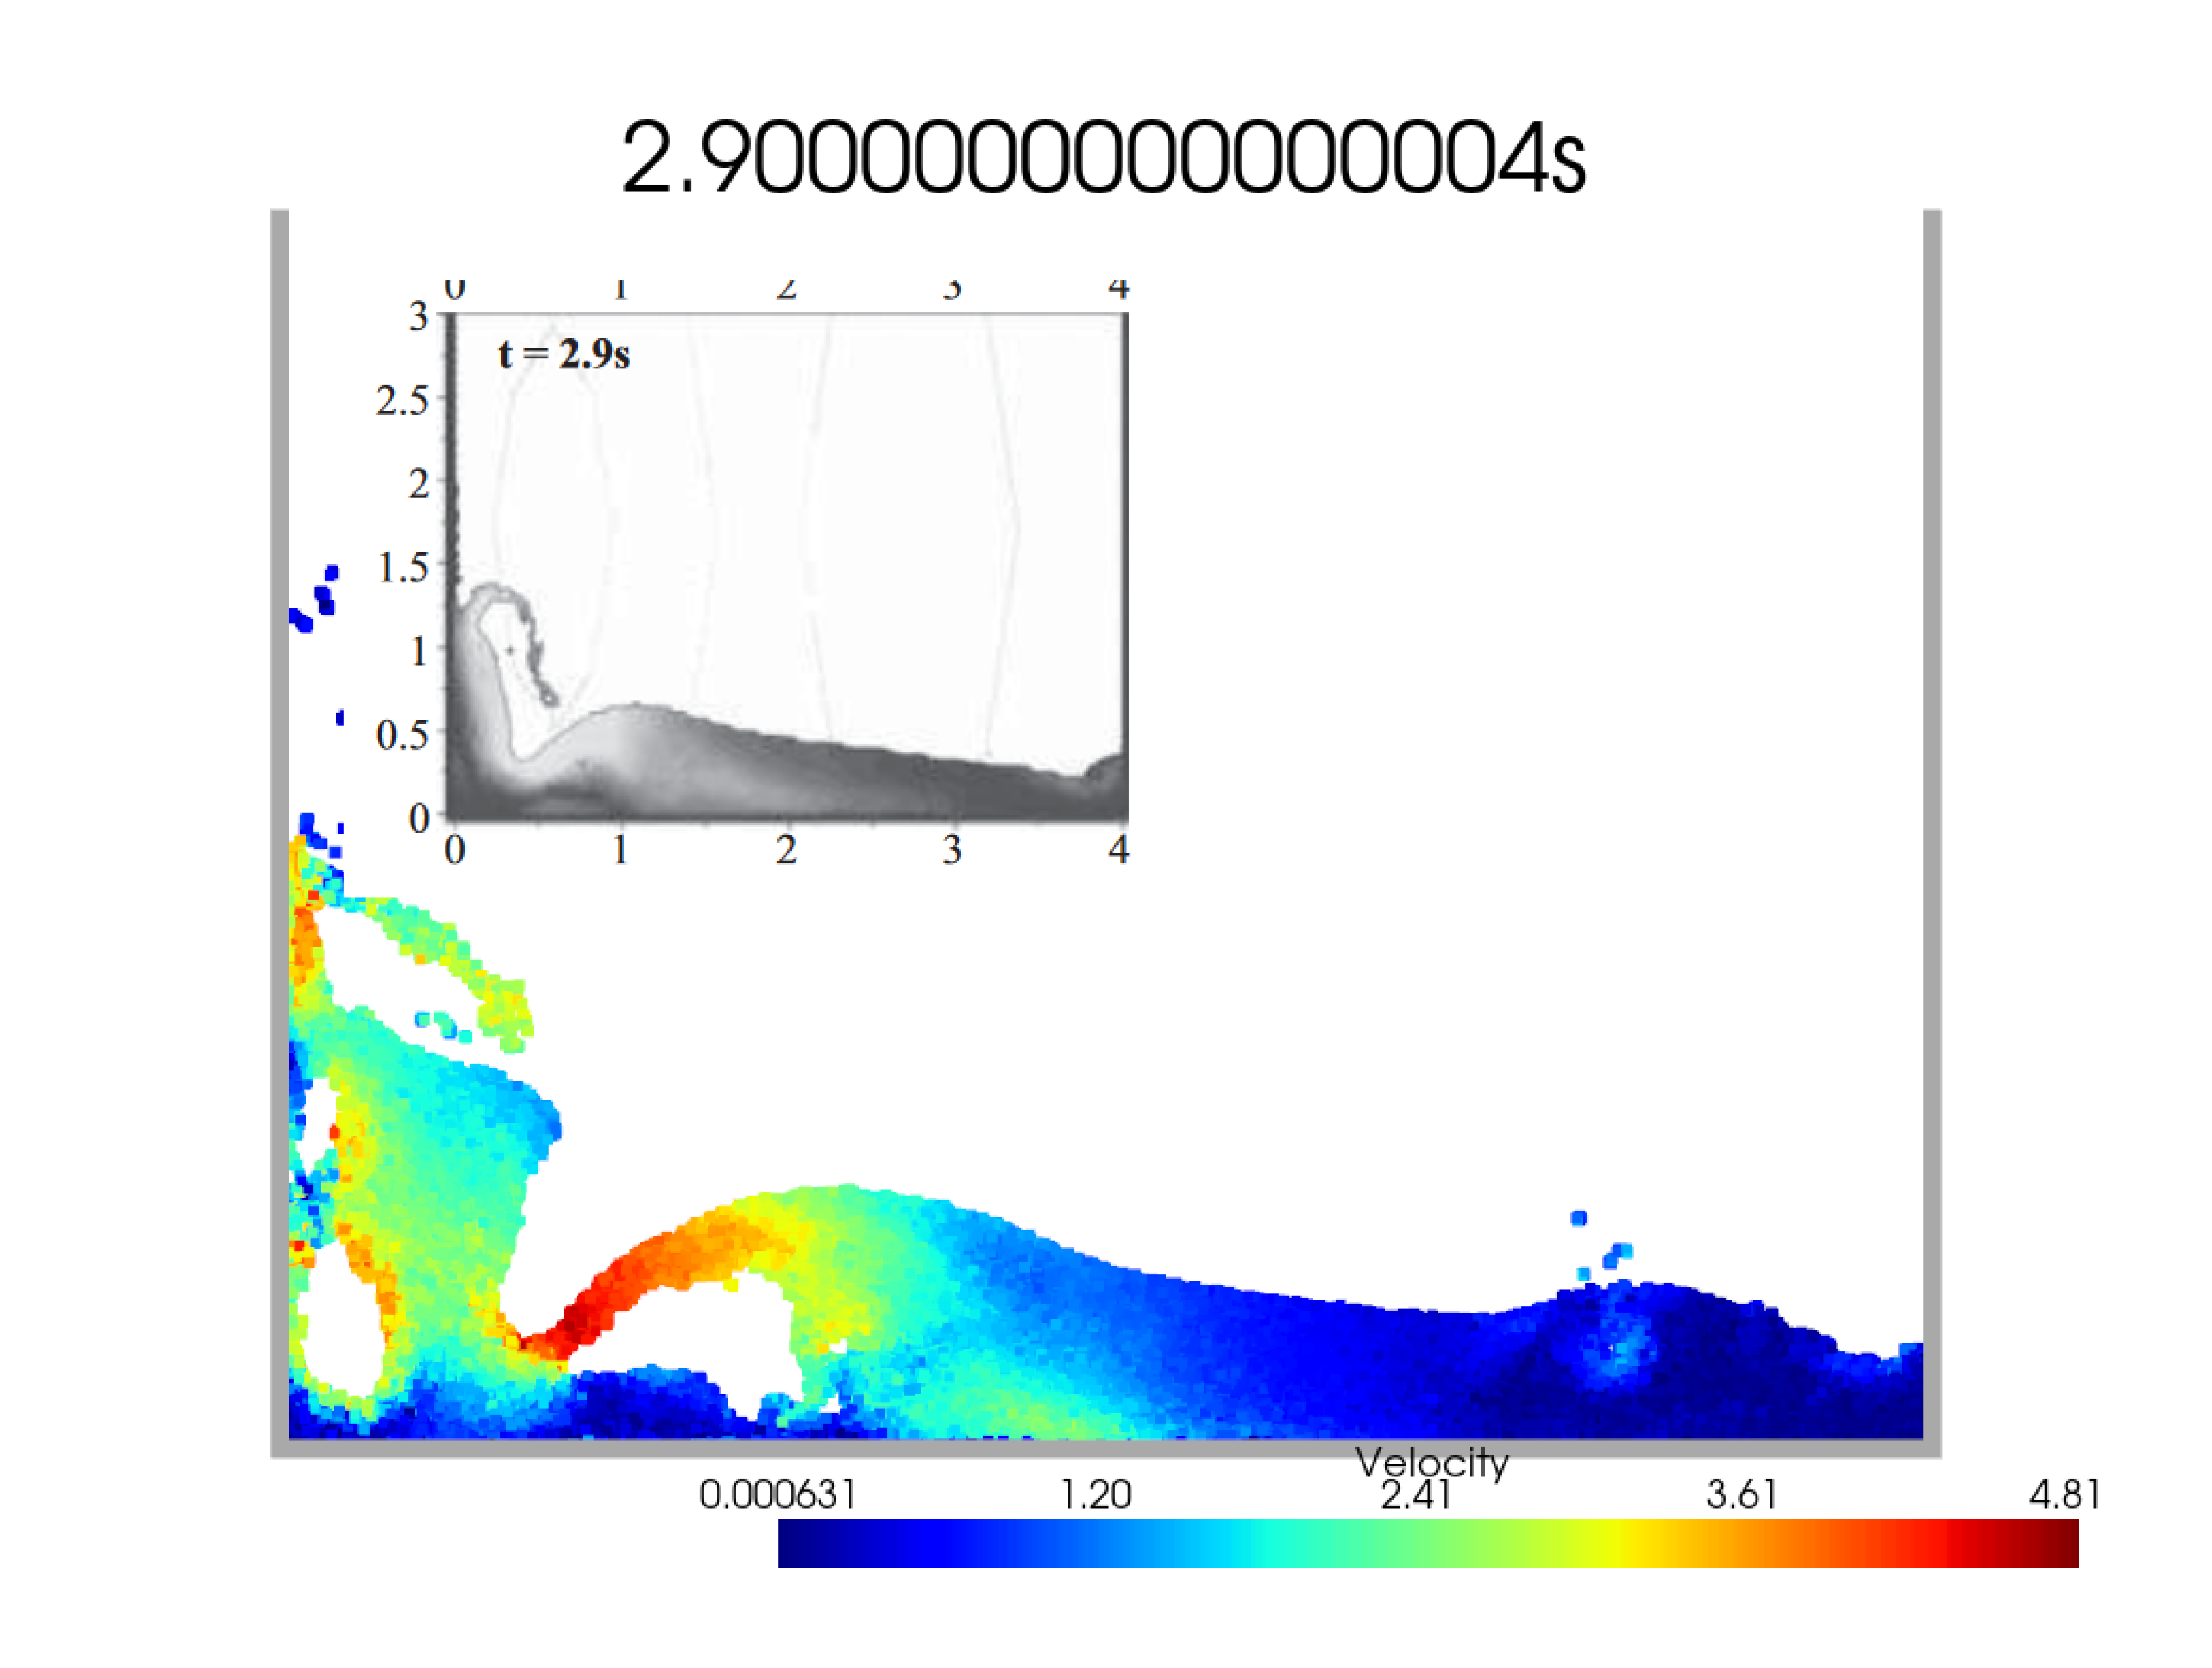
\includegraphics[width=0.47\textwidth]{images/CollapseDry/half/collapse_dry29_combined.png}
        }
    \end{figure}
\end{frame}

\begin{frame}
    在这个算例中,
    标准算例提供的图片并没有明确指出壁面是怎么处理的(因为书中都是讲完三四种壁面方法,
    最后才提供算例的结果),
    但并不在算例中指出采用了什么壁面条件。
    算例从液体回注开始,和标准算例差别比较大,
    但在垮塌过程中曲线对比能对上。
    \begin{figure}[H]
        \centering
        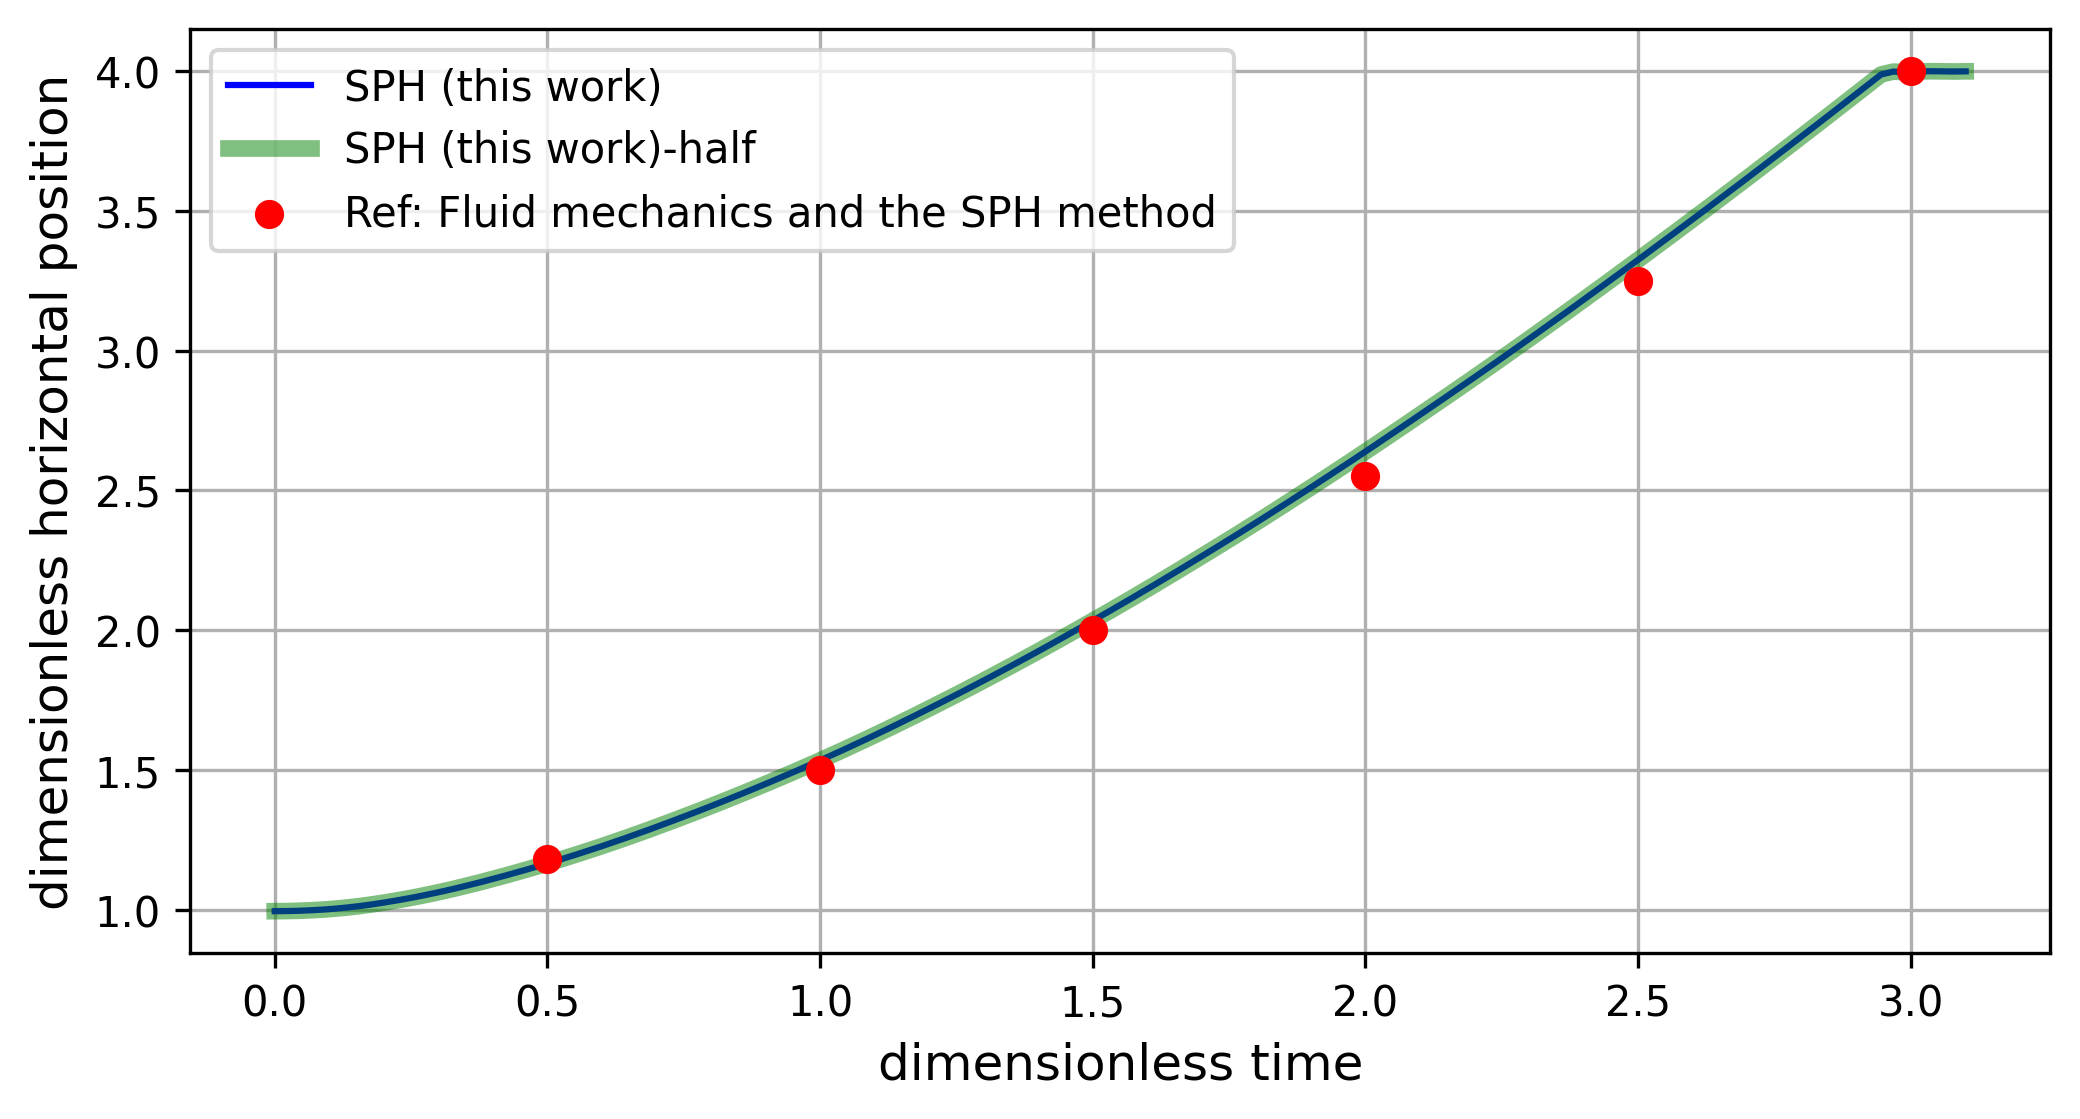
\includegraphics[width=\textwidth]{images/CollapseDry/horizontal_position.png}
    \end{figure}
\end{frame}

\begin{frame}
    \begin{figure}[H]
        \centering
        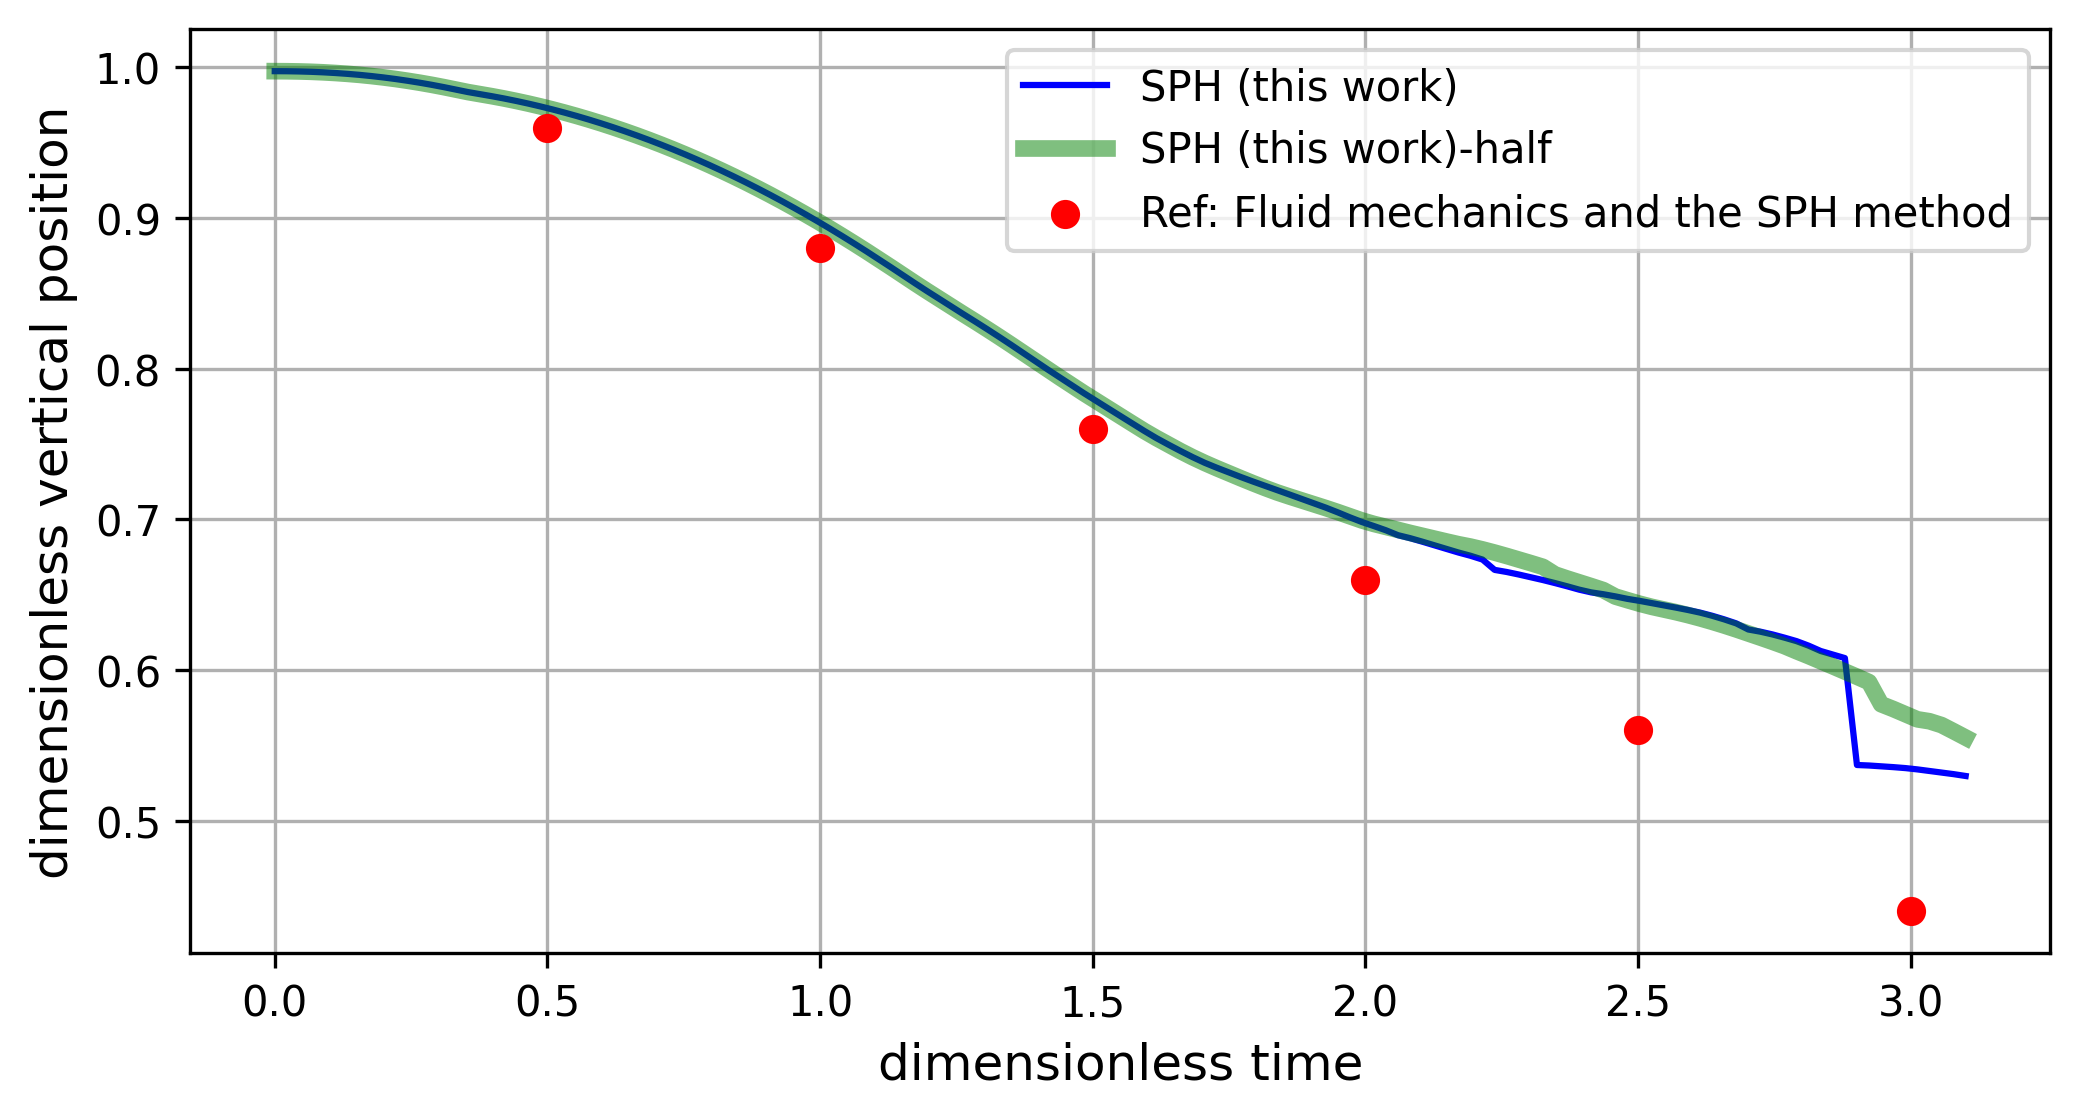
\includegraphics[width=\textwidth]{images/CollapseDry/vertical_position.png}
    \end{figure}
\end{frame}
\section{液柱垮塌——实验对比以及不同粘度}

\begin{frame}
    \frametitle{\secname}
    \framesubtitle{实验对比}
    \begin{figure}[H]
        \centering
        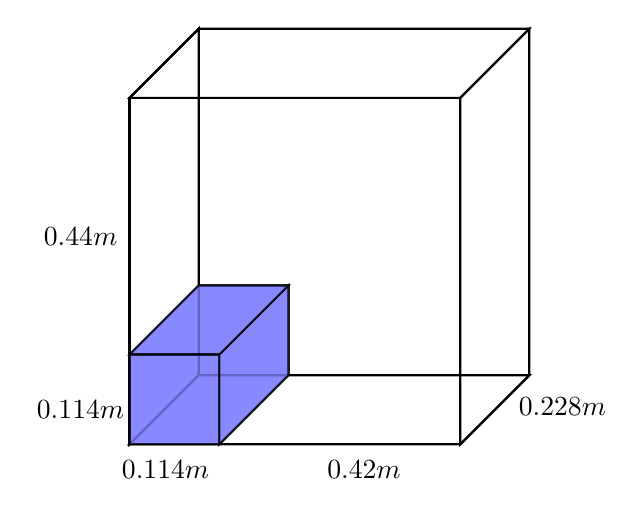
\begin{tikzpicture}
            % a box in 3D space
            % 0.42 width
            % 0.44 height
            % 0.228 depth
            \def\x{0.42*10}
            \def\y{0.44*10}
            \def\z{0.228*10}
            \draw[thick] (0,0,0)--(\x,0,0)--(\x,\y,0)--(0,\y,0)--cycle;
            \draw[thick] (0,0,0)--(0,0,\z)--(0,\y,\z)--(0,\y,0)--cycle;
            \draw[thick] (0,0,0)--(\x,0,0)--(\x,0,\z)--(0,0,\z)--cycle;
            \draw[thick] (\x,0,0)--(\x,\y,0)--(\x,\y,\z)--(\x,0,\z)--cycle;
            \draw[thick] (0,\y,0)--(\x,\y,0)--(\x,\y,\z)--(0,\y,\z)--cycle;
            \draw[thick] (0,0,\z)--(\x,0,\z)--(\x,\y,\z)--(0,\y,\z)--cycle;

            % draw water column
            % initial size is 0.114*0.114*0.228
            % from (0, 0, 0)
            \def\waterx{0.114*10}
            \def\watery{0.114*10}
            \def\waterz{0.228*10}
            \draw[thick,fill=blue!50, opacity=0.75] (0,0,0)--(\waterx,0,0)--(\waterx,\watery,0)--(0,\watery,0)--cycle;
            \draw[thick,fill=blue!50, opacity=0.75] (0,0,0)--(0,0,\waterz)--(0,\watery,\waterz)--(0,\watery,0)--cycle;
            \draw[thick,fill=blue!50, opacity=0.75] (0,0,0)--(\waterx,0,0)--(\waterx,0,\waterz)--(0,0,\waterz)--cycle;
            \draw[thick,fill=blue!50, opacity=0.75] (\waterx,0,0)--(\waterx,\watery,0)--(\waterx,\watery,\waterz)--(\waterx,0,\waterz)--cycle;
            \draw[thick,fill=blue!50, opacity=0.75] (0,\watery,0)--(\waterx,\watery,0)--(\waterx,\watery,\waterz)--(0,\watery,\waterz)--cycle;
            \draw[thick,fill=blue!50, opacity=0.75] (0,0,\waterz)--(\waterx,0,\waterz)--(\waterx,\watery,\waterz)--(0,\watery,\waterz)--cycle;

            % denote the size
            \node at (0.5*\x, -1.2) {$0.42m$};
            \node at (-1.5, 0.4*\y) {$0.44m$};
            \node at (1.1*\x, -0.4) {$0.228m$};
            \node at (-0.1*\x, -1.2) {$0.114m$};
            \node at (-1.5, -0.1*\y) {$0.114m$};
        \end{tikzpicture}
    \end{figure}
\end{frame}

\begin{frame}
    Cruchaga, 2007所做的实验图片,
    原文基于界面捕捉的 FEM。
    \begin{figure}[H]
        \centering
        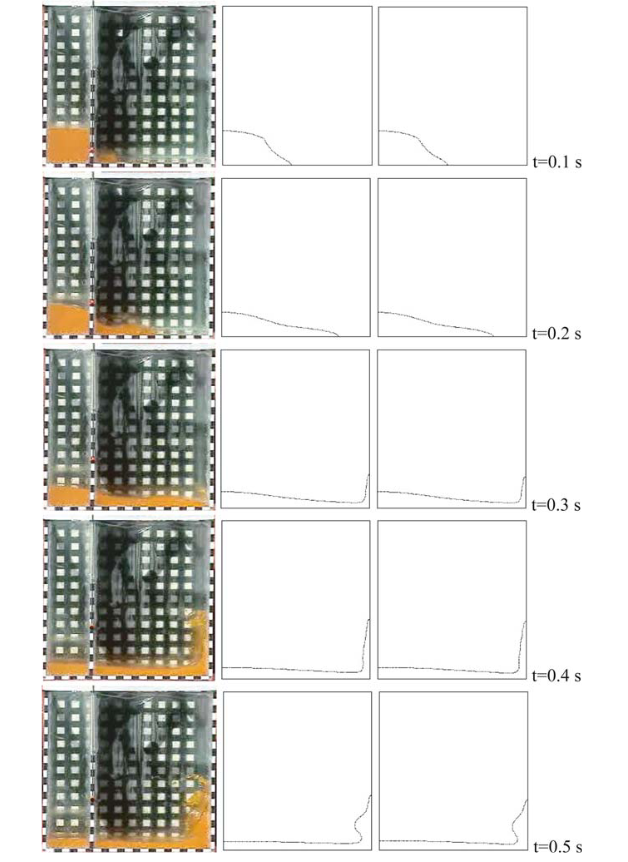
\includegraphics[width=0.5\textwidth]{images/Cruchaga/cruchaga_experiment.png}
    \end{figure}
\end{frame}

\begin{frame}
    \begin{figure}[H]
        \centering
        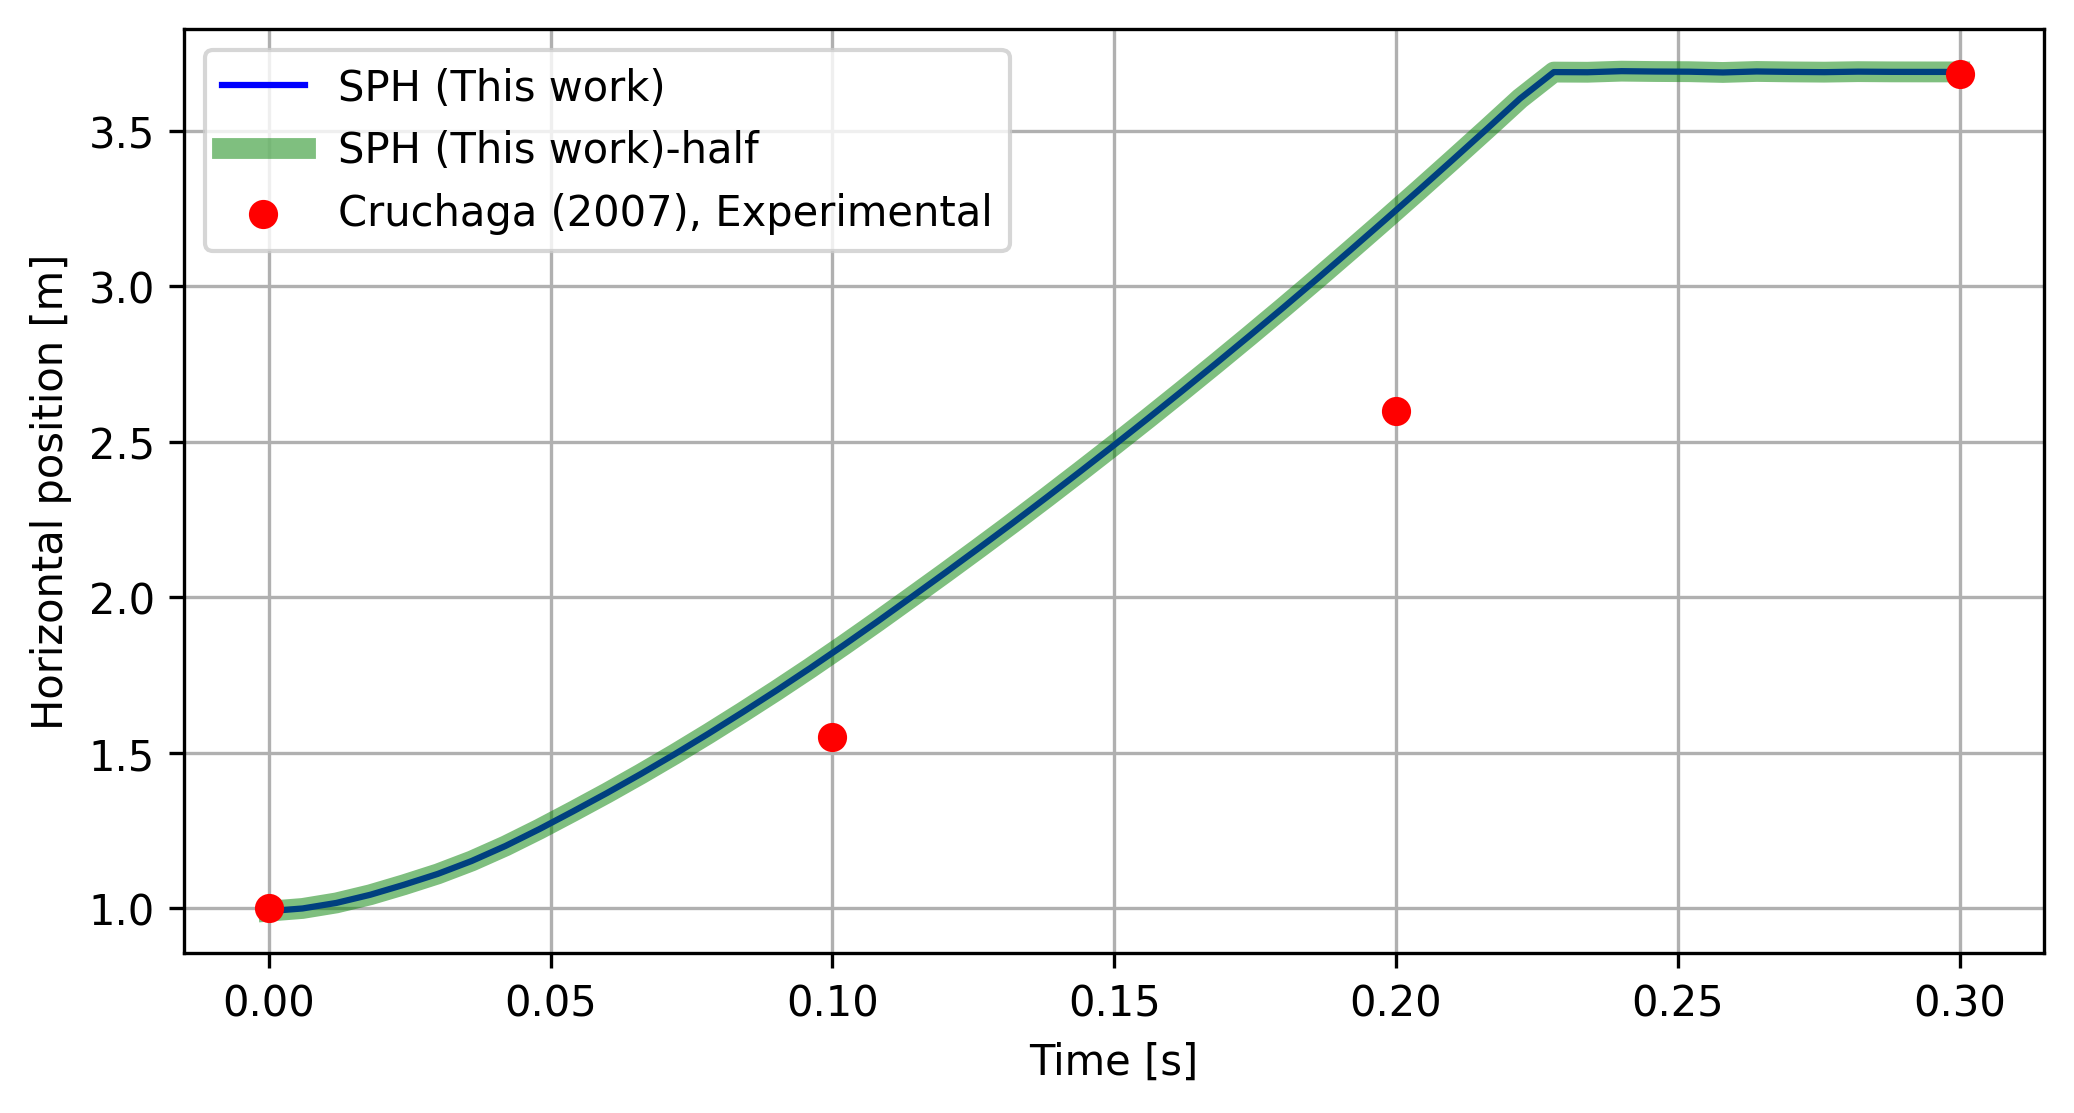
\includegraphics[width=\textwidth]{images/Cruchaga/2d/cruchaga_2d.png}
    \end{figure}
    因为差别不大所以只展示不垫高壁面粒子的情形动画。
\end{frame}

\begin{frame}
    同时我还计算了三维情形下的液柱垮塌,
    使用了 1.6 万个粒子,大概计算了 1.5 小时。
    就计算结果而言我认为三维的 SPH 和二维的 SPH 差别很大,三维更准。
    同时壁面粘性还是存在问题,有可能是粒子数不够——$20\times 20\times 40$,
    或者壁面摩擦模型有问题。
    另外我还计算了一个很黏的情况,$\mu=8kg/(m\cdot s)$,但和Cruchaga对不上。
    \begin{figure}[H]
        \centering
        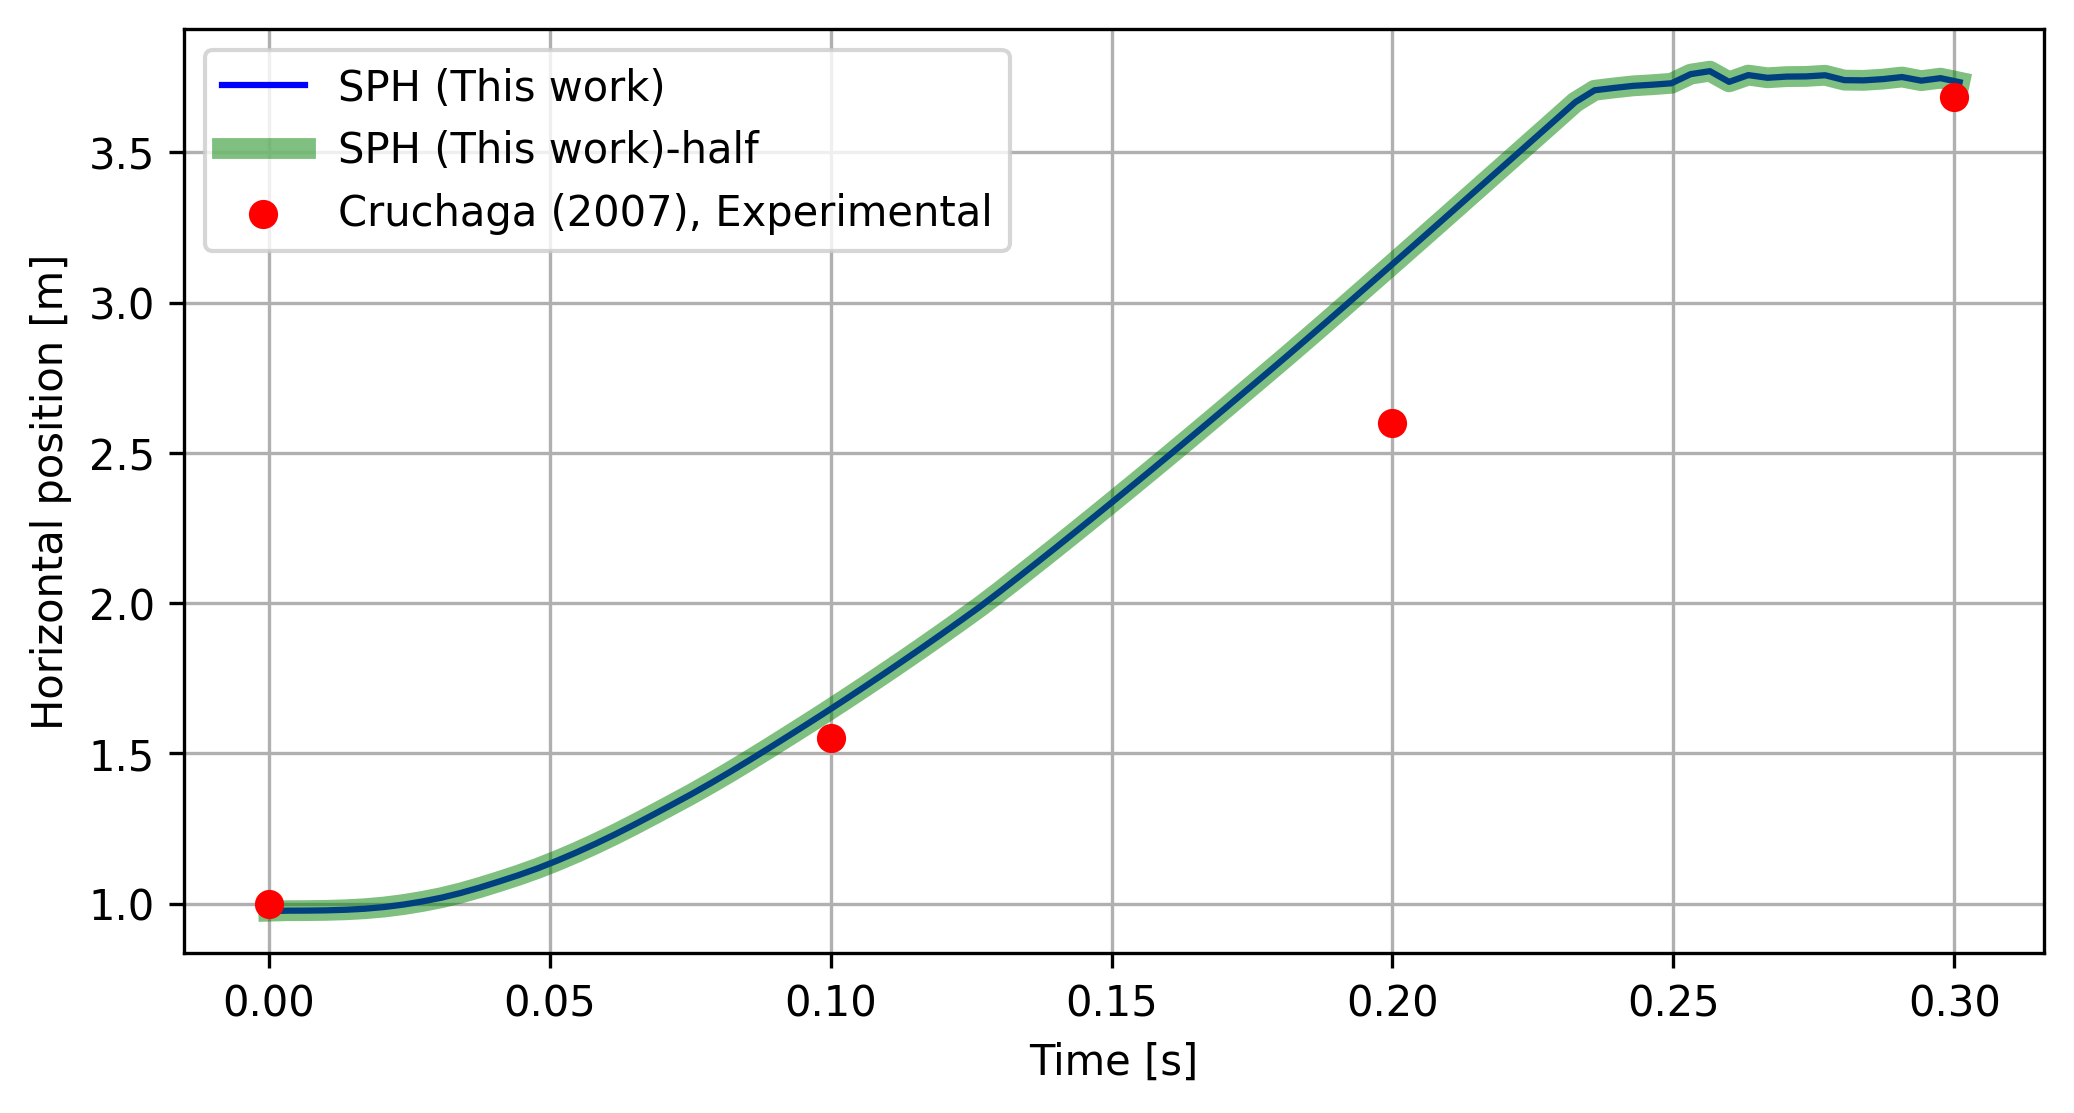
\includegraphics[width=\textwidth]{images/Cruchaga/3d/cruchaga_3d.png}
    \end{figure}
\end{frame}
\section{顶盖驱动方腔流}

\begin{frame}
    \begin{figure}[H]
        \centering
        \begin{tikzpicture}
            % lid driven cavity
            % draw a box
            \def\boxlength{5}
            \draw[-] (0,0)--(0,\boxlength)--(\boxlength,\boxlength)--(\boxlength,0)--cycle;
            \node at (0.5*\boxlength, -0.5) {$L$};
            \node at (-0.5, 0.5*\boxlength) {$L$};

            % u velocity
            \node at (0.5*\boxlength, 1.05*\boxlength) {$\vec{u}=1\vec{i}\rightarrow$};
            % left 3 side u = 0
            \node at (0.5, 0.5*\boxlength) {$\vec{u}=\vec{0}$};
            \node at (\boxlength-0.5, 0.5*\boxlength) {$\vec{u}=\vec{0}$};
            \node at (0.5*\boxlength, 0.5) {$\vec{u}=\vec{0}$};

            % a vortex in center of the box
            \draw[->] (0.2*\boxlength, 0.9*\boxlength) -- (0.8*\boxlength, 0.9*\boxlength);
            % draw a curve backward
            \draw[->] (0.8*\boxlength, 0.9*\boxlength) .. controls (0.7*\boxlength, 0.6*\boxlength) and (0.4*\boxlength, 0.8*\boxlength) .. (0.2*\boxlength, 0.9*\boxlength);
        \end{tikzpicture}
    \end{figure}
\end{frame}

\begin{frame}
    对于该问题的边界处理,
    我直接在壁面上布置了定速且不变位置的边界粒子,
    因为该问题流体环境致密,
    所以壁面粒子对于水体粒子有:
    强制力,压力和粘性力。
    $Re=100$:
    \begin{figure}[H]
        \centering
        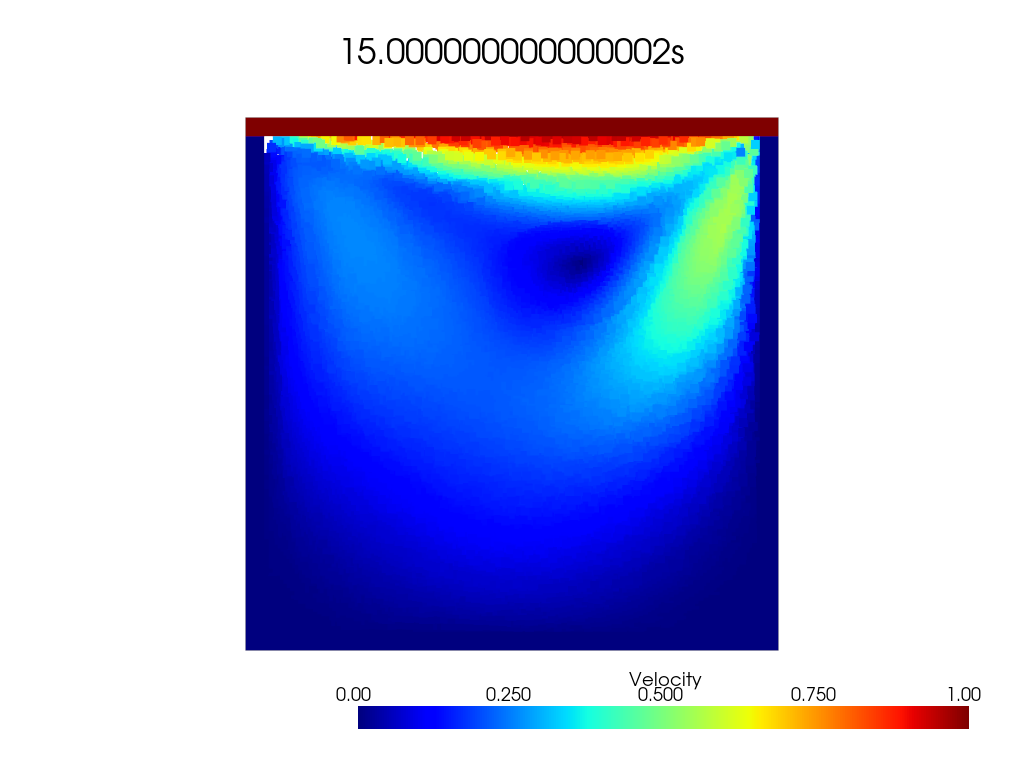
\includegraphics[width=0.8\textwidth]{images/LidDrivenCavity/Re100/lid_driven_cavity_re100.png}
    \end{figure}
\end{frame}

\begin{frame}
    \begin{figure}[H]
        \centering
        \subfigure[$N=50$]{
            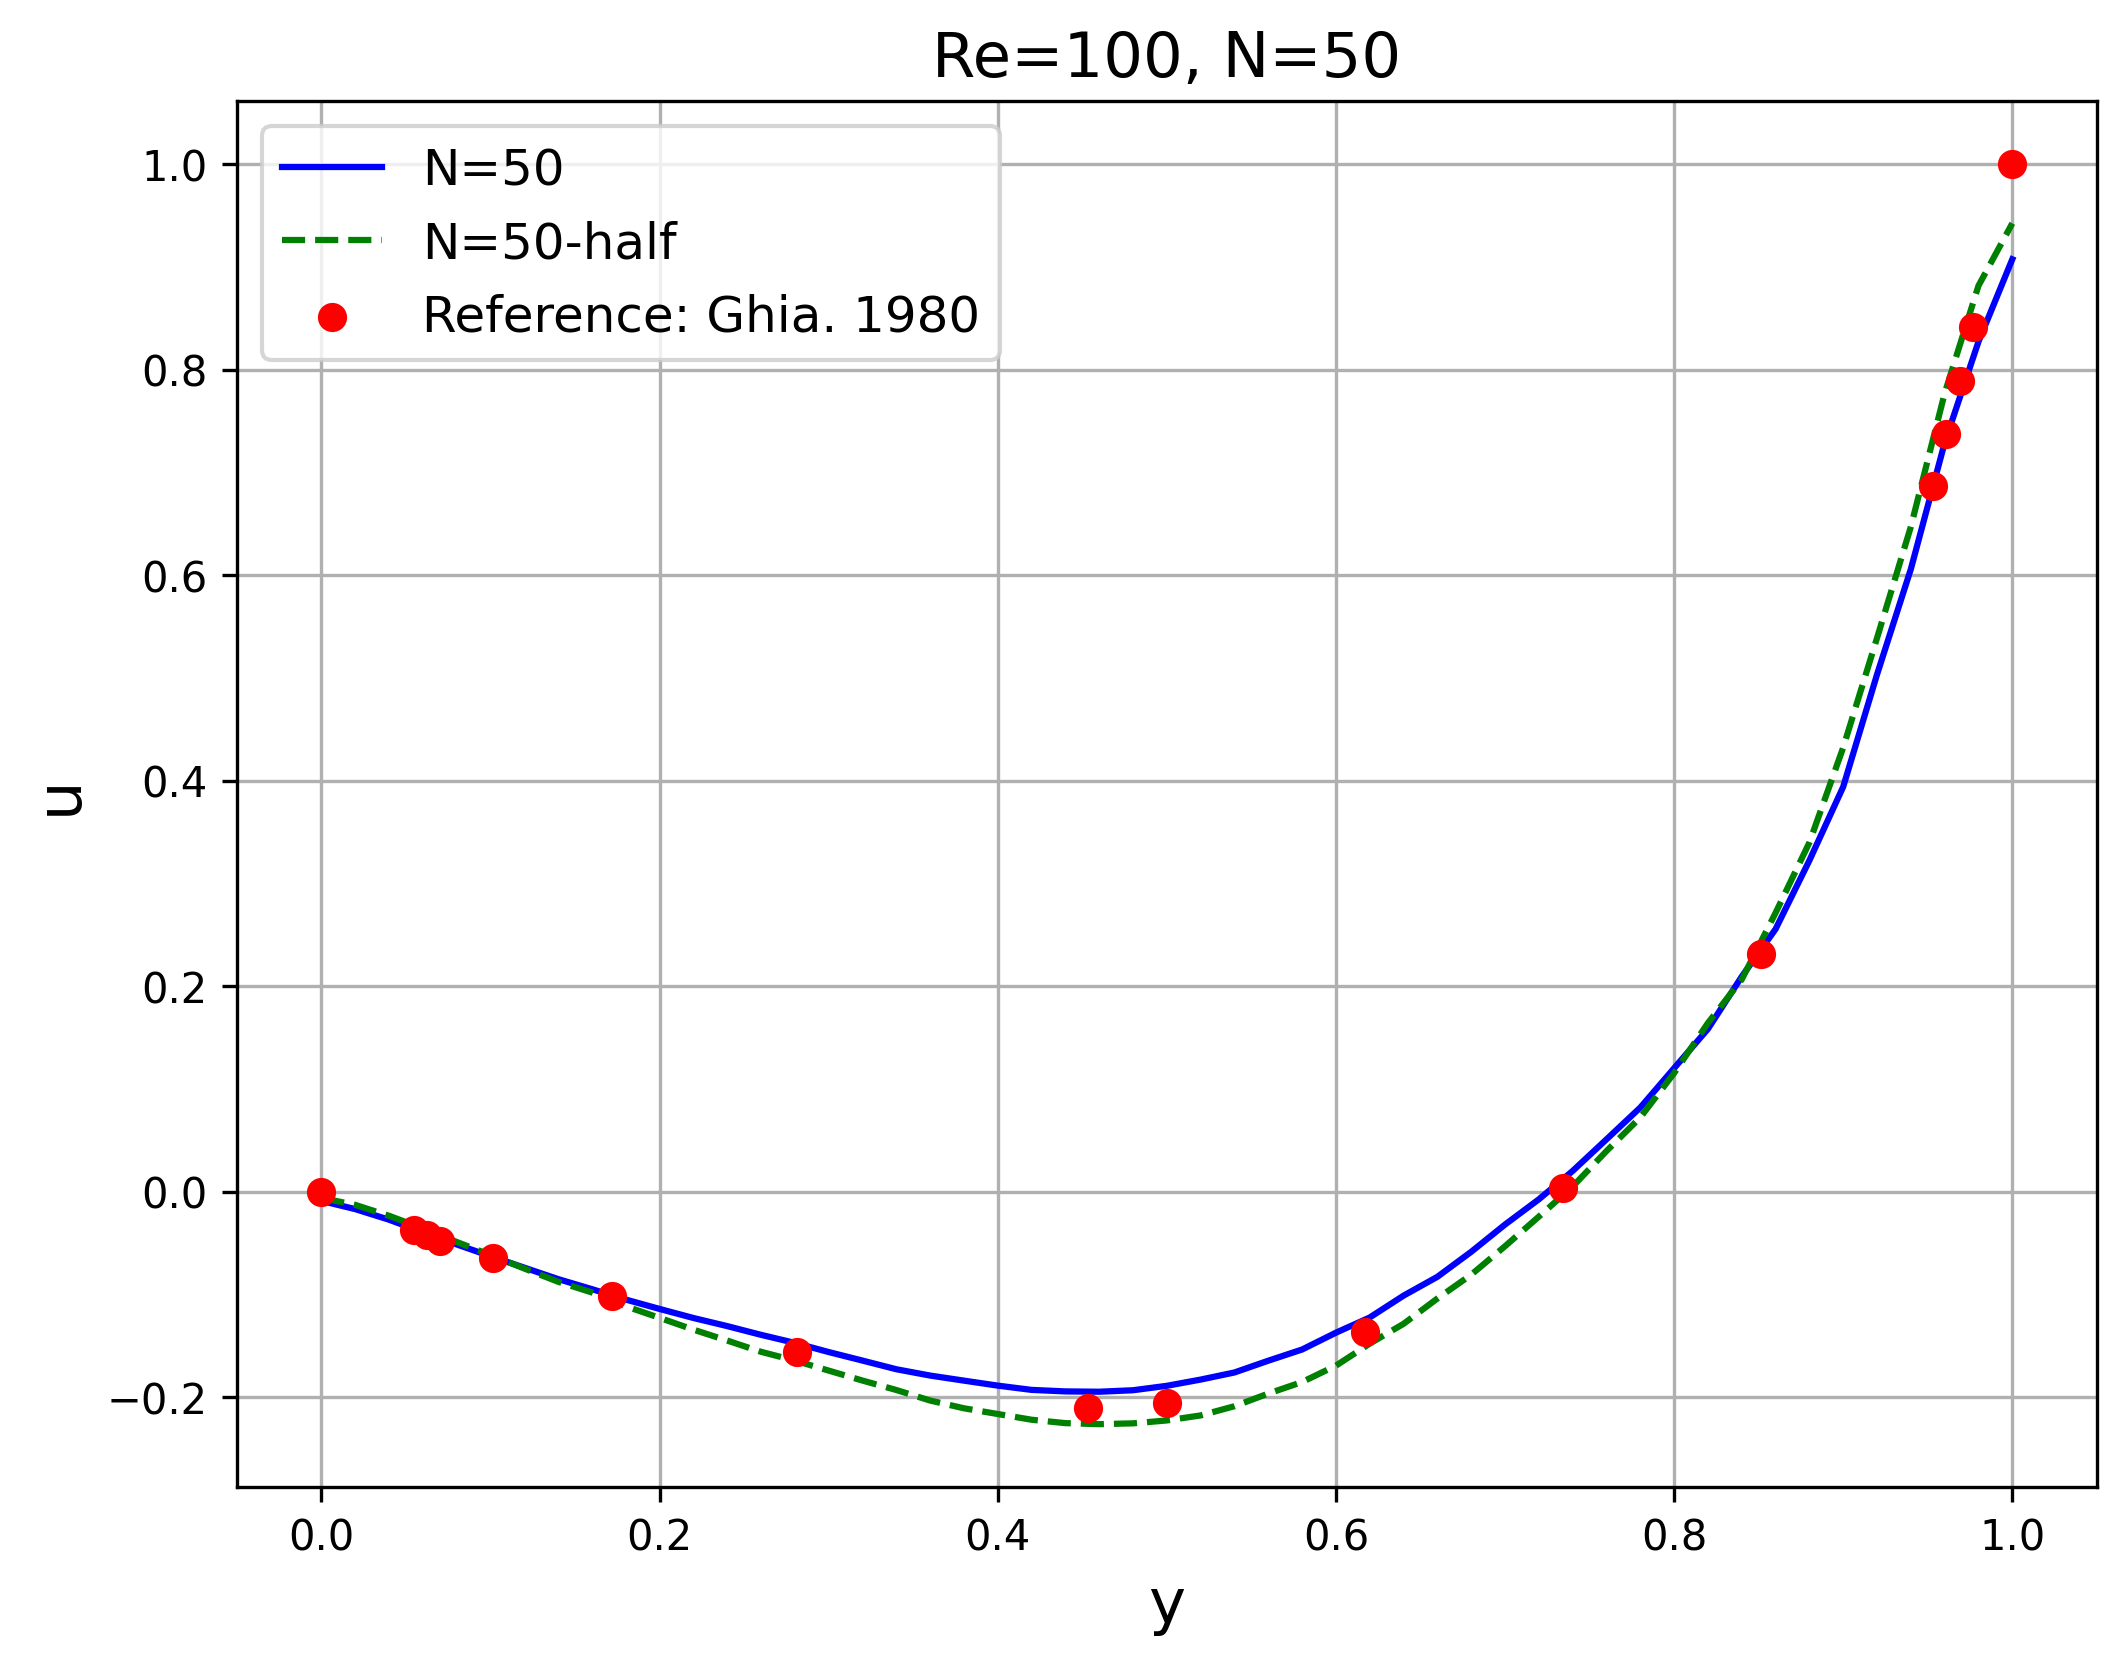
\includegraphics[width=0.45\textwidth]{images/LidDrivenCavity/Re100/u_middle_re100_N50.png}
        }
        \subfigure[$N=100$]{
            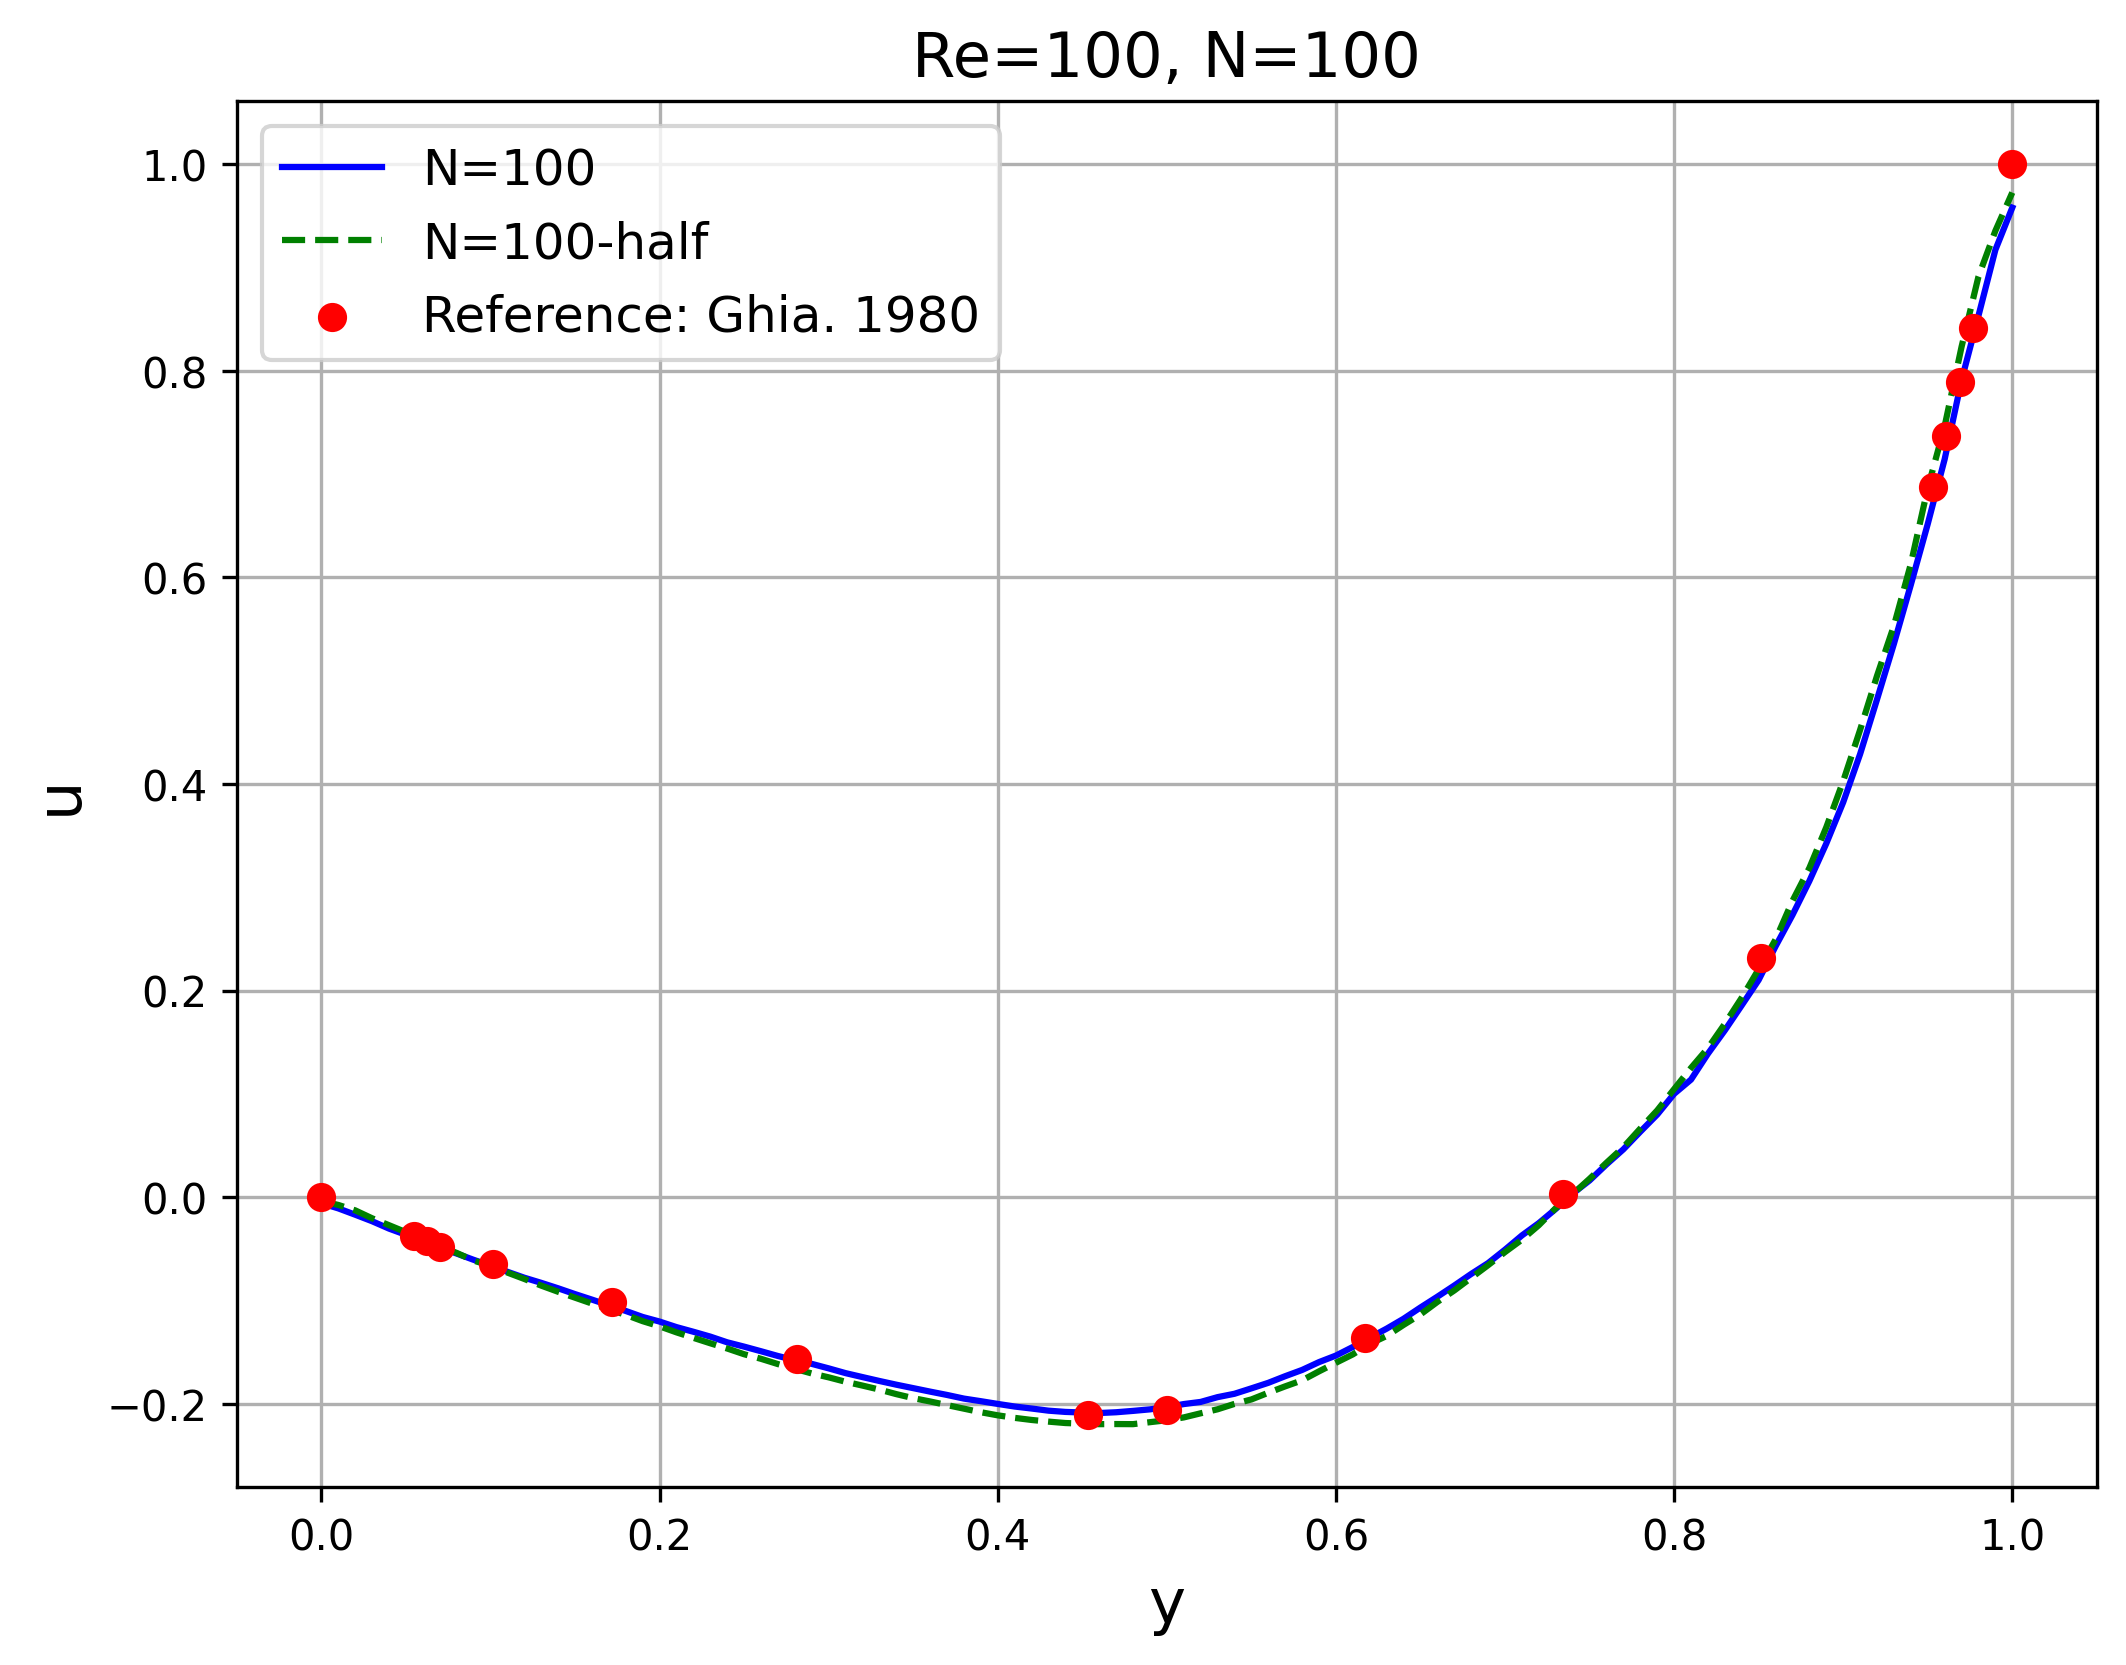
\includegraphics[width=0.45\textwidth]{images/LidDrivenCavity/Re100/u_middle_re100_N100.png}
        }
    \end{figure}
\end{frame}

\begin{frame}
    \begin{figure}[H]
        \centering
        \subfigure[$N=50$]{
            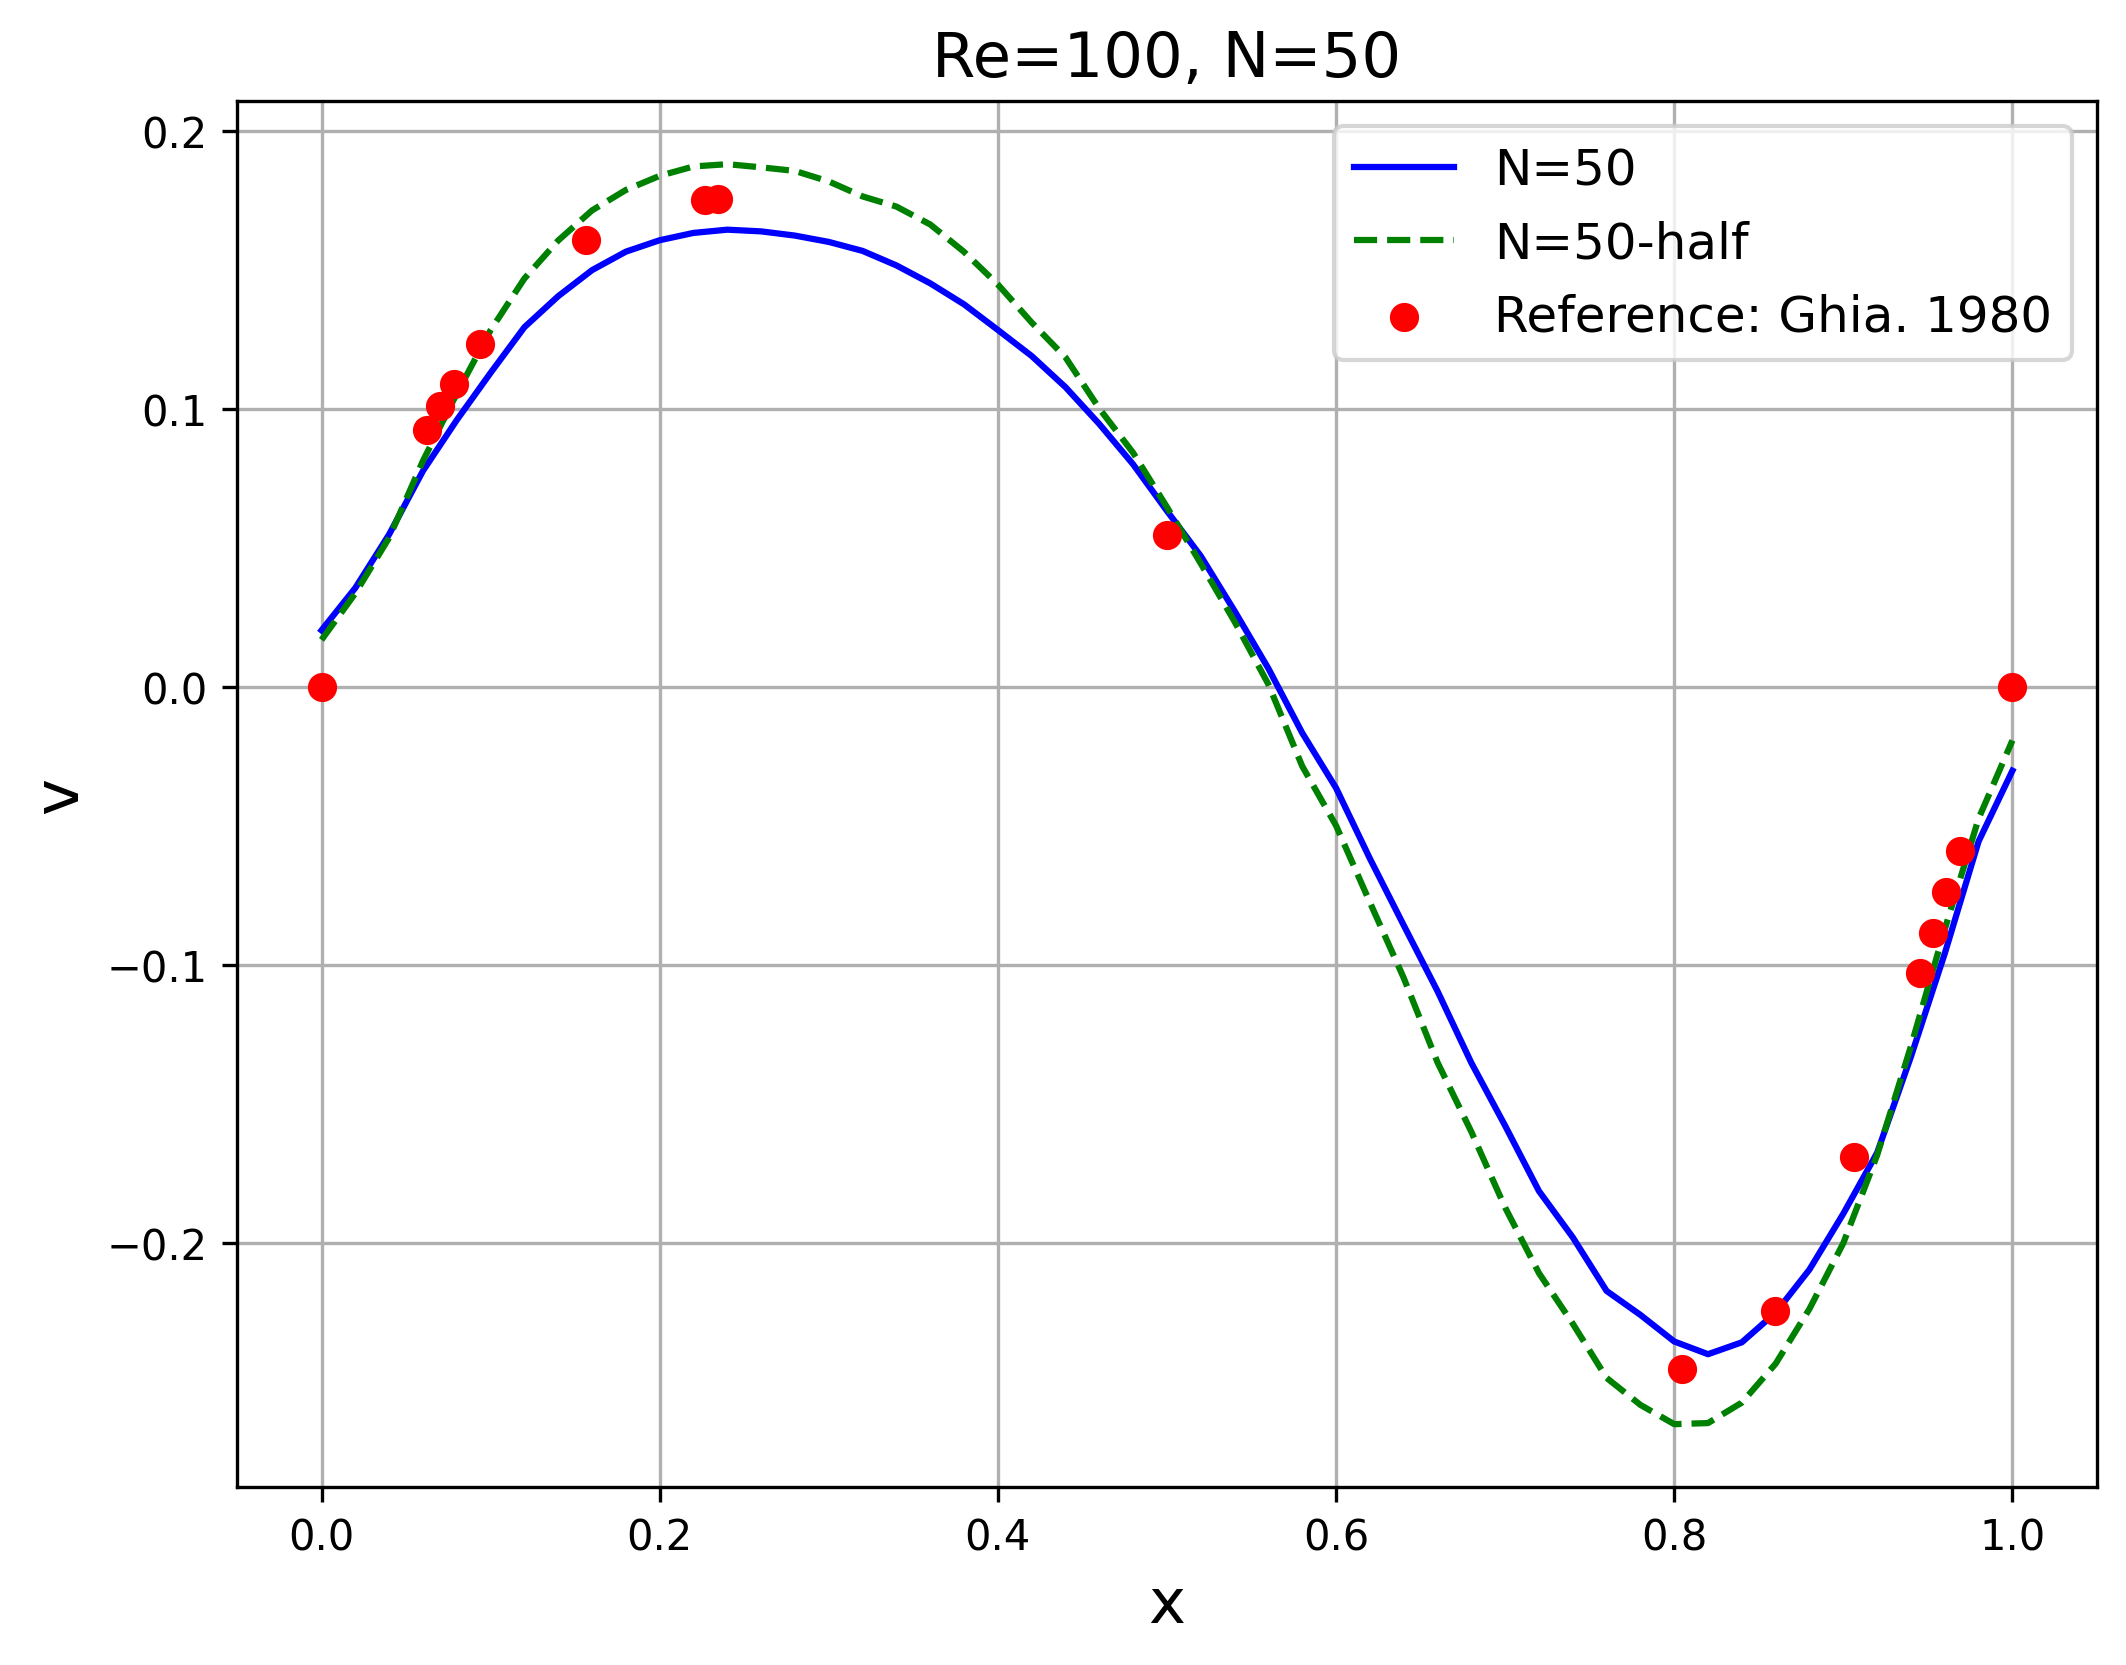
\includegraphics[width=0.45\textwidth]{images/LidDrivenCavity/Re100/v_middle_re100_N50.png}
        }
        \subfigure[$N=100$]{
            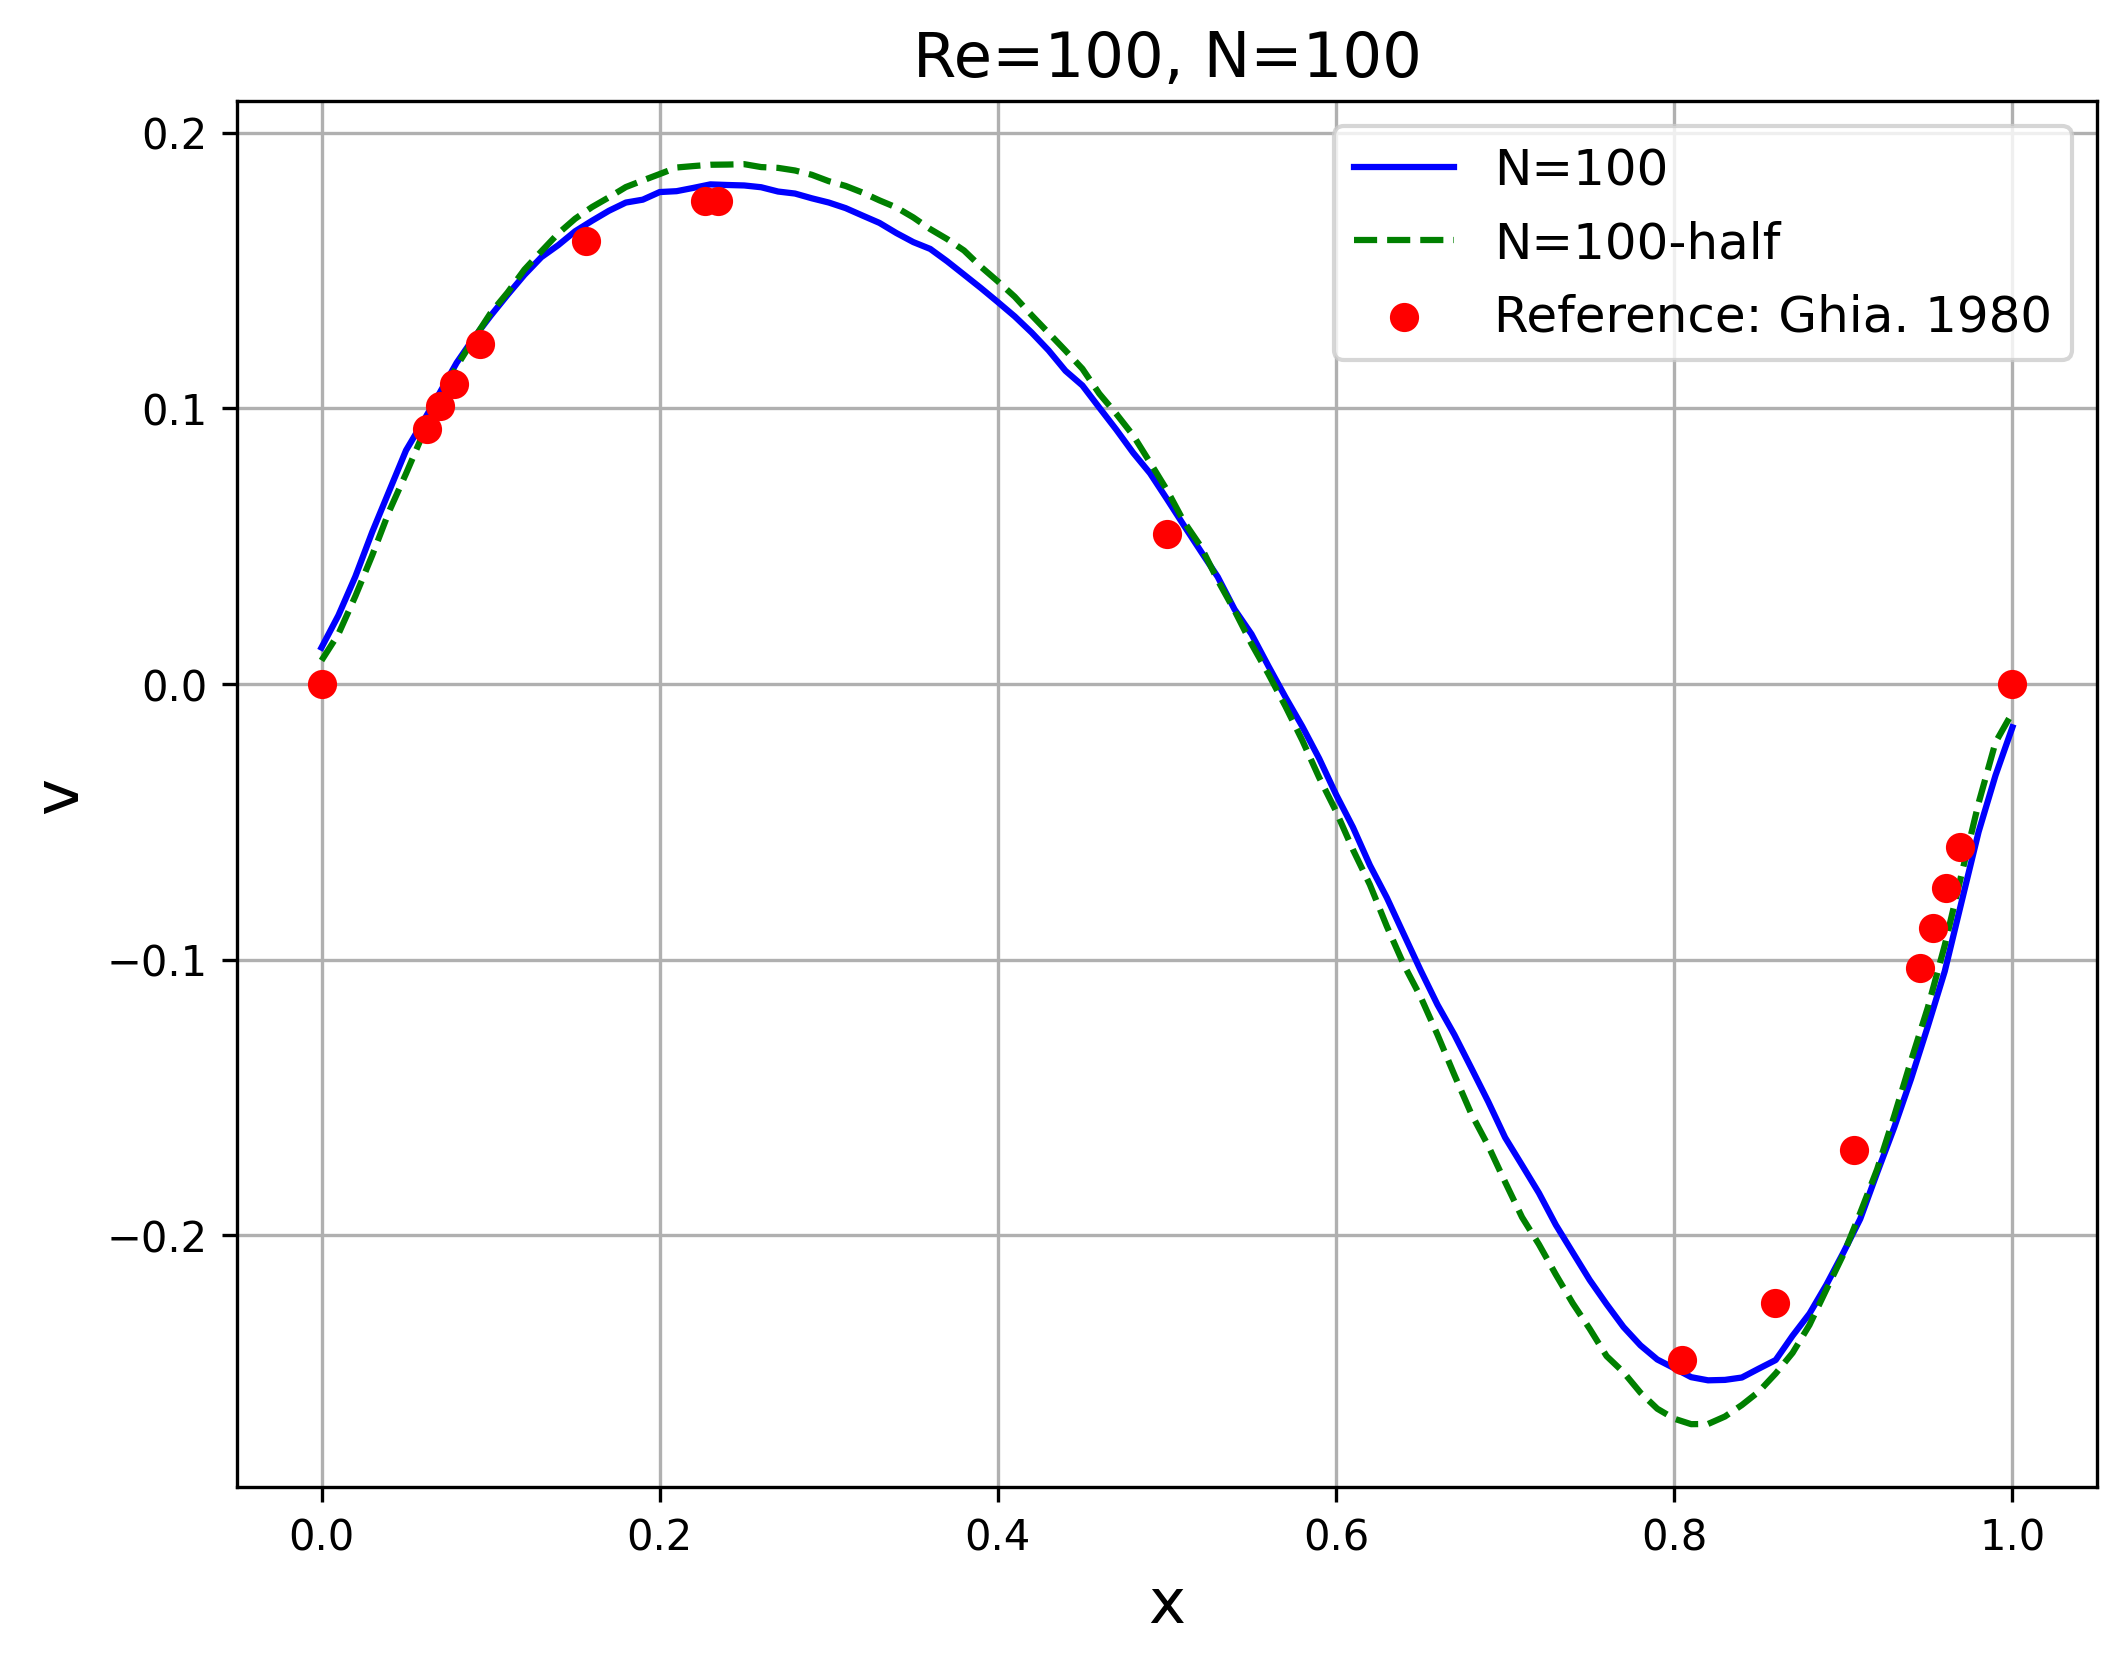
\includegraphics[width=0.45\textwidth]{images/LidDrivenCavity/Re100/v_middle_re100_N100.png}
        }
    \end{figure}
\end{frame}

\begin{frame}
    $Re=400$:
    \begin{figure}[H]
        \centering
        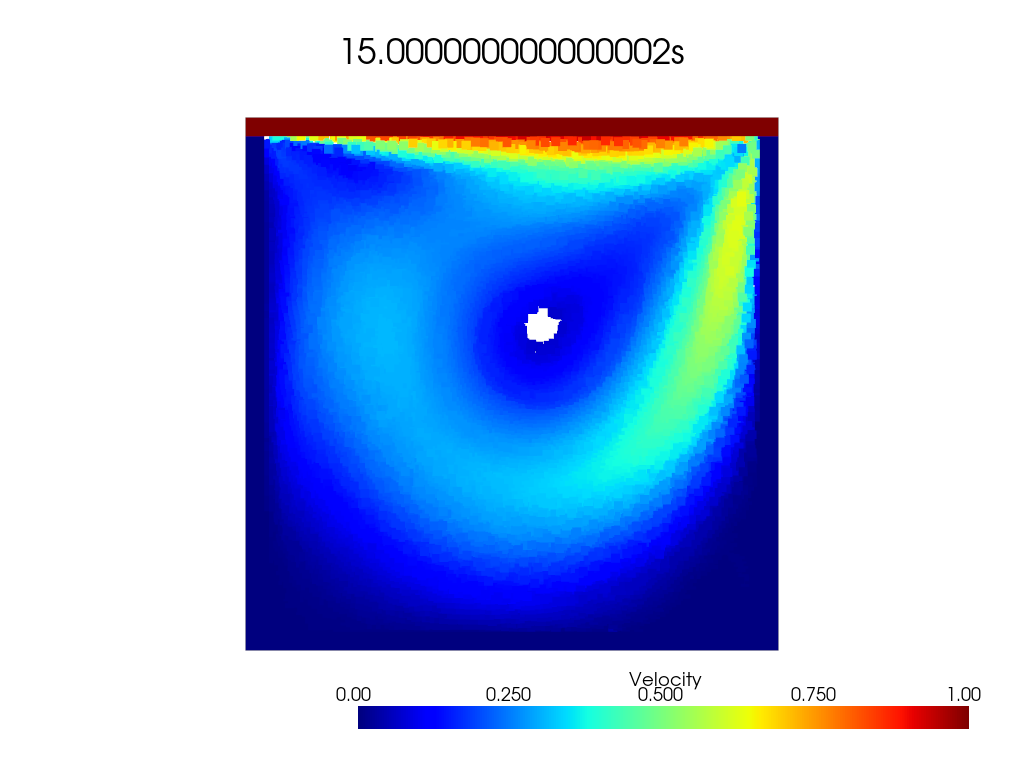
\includegraphics[width=0.8\textwidth]{images/LidDrivenCavity/Re400/lid_driven_cavity_re400.png}
    \end{figure}
\end{frame}

\begin{frame}
    \begin{figure}[H]
        \centering
        \subfigure[$N=50$]{
            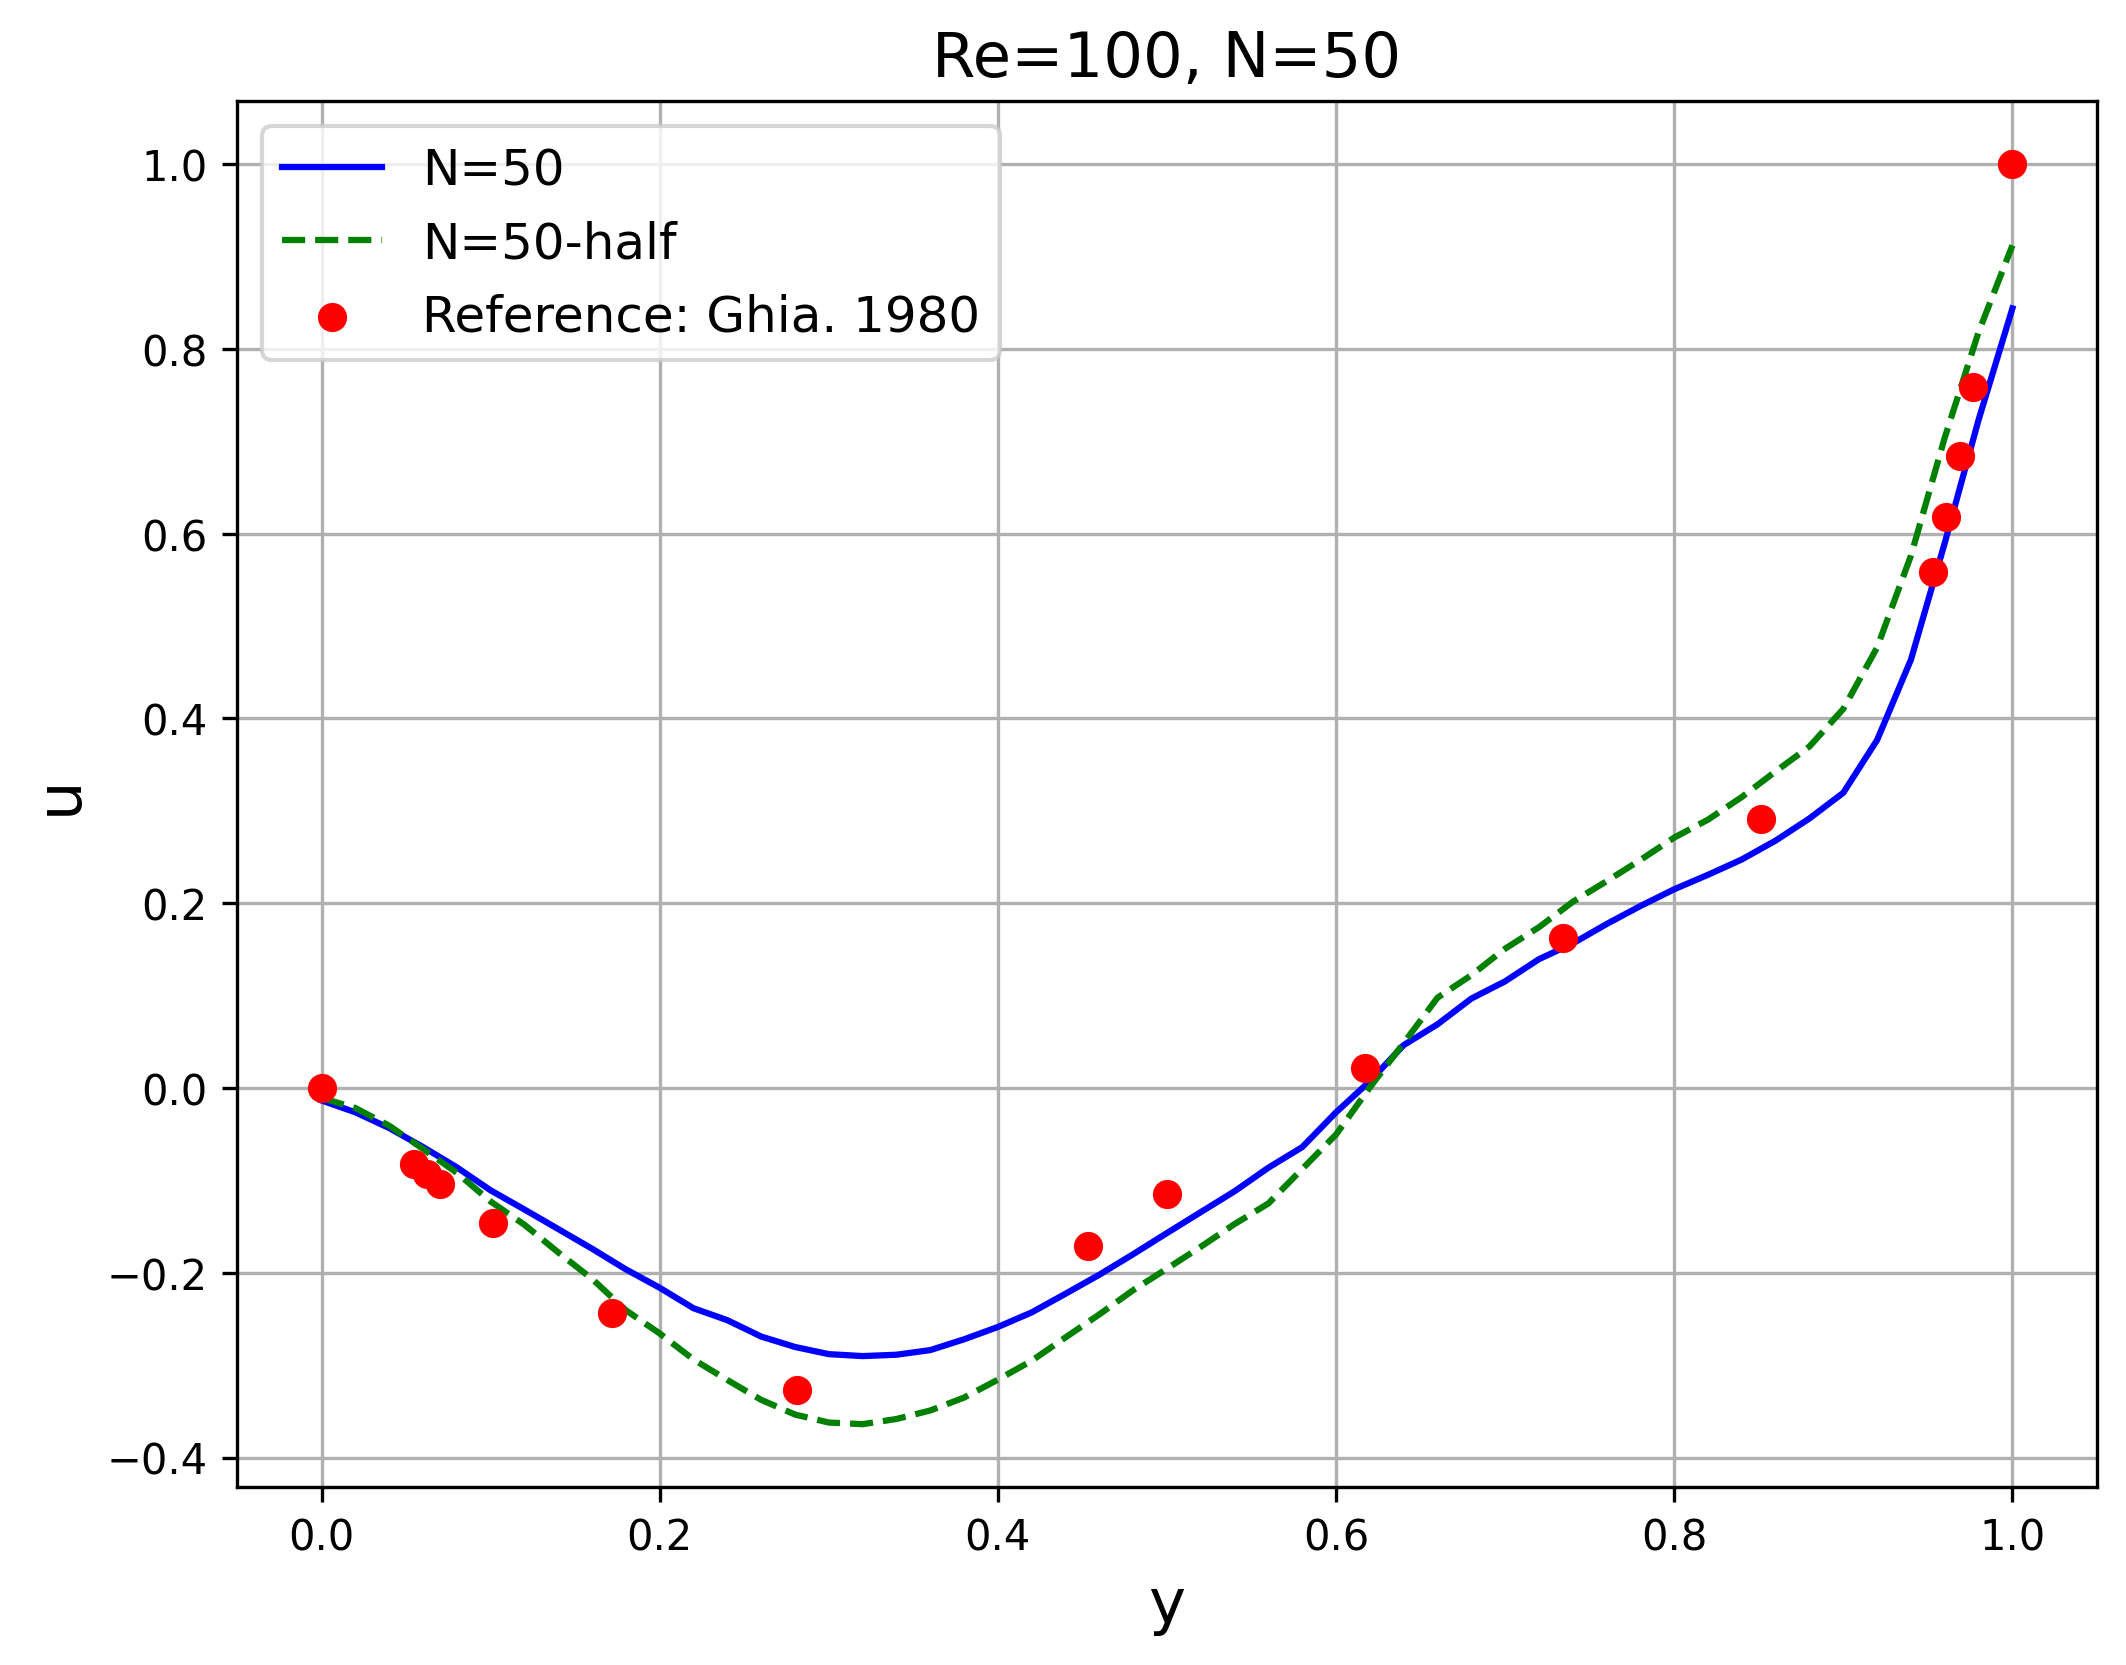
\includegraphics[width=0.45\textwidth]{images/LidDrivenCavity/Re400/u_middle_re400_N50.png}
        }
        \subfigure[$N=100$]{
            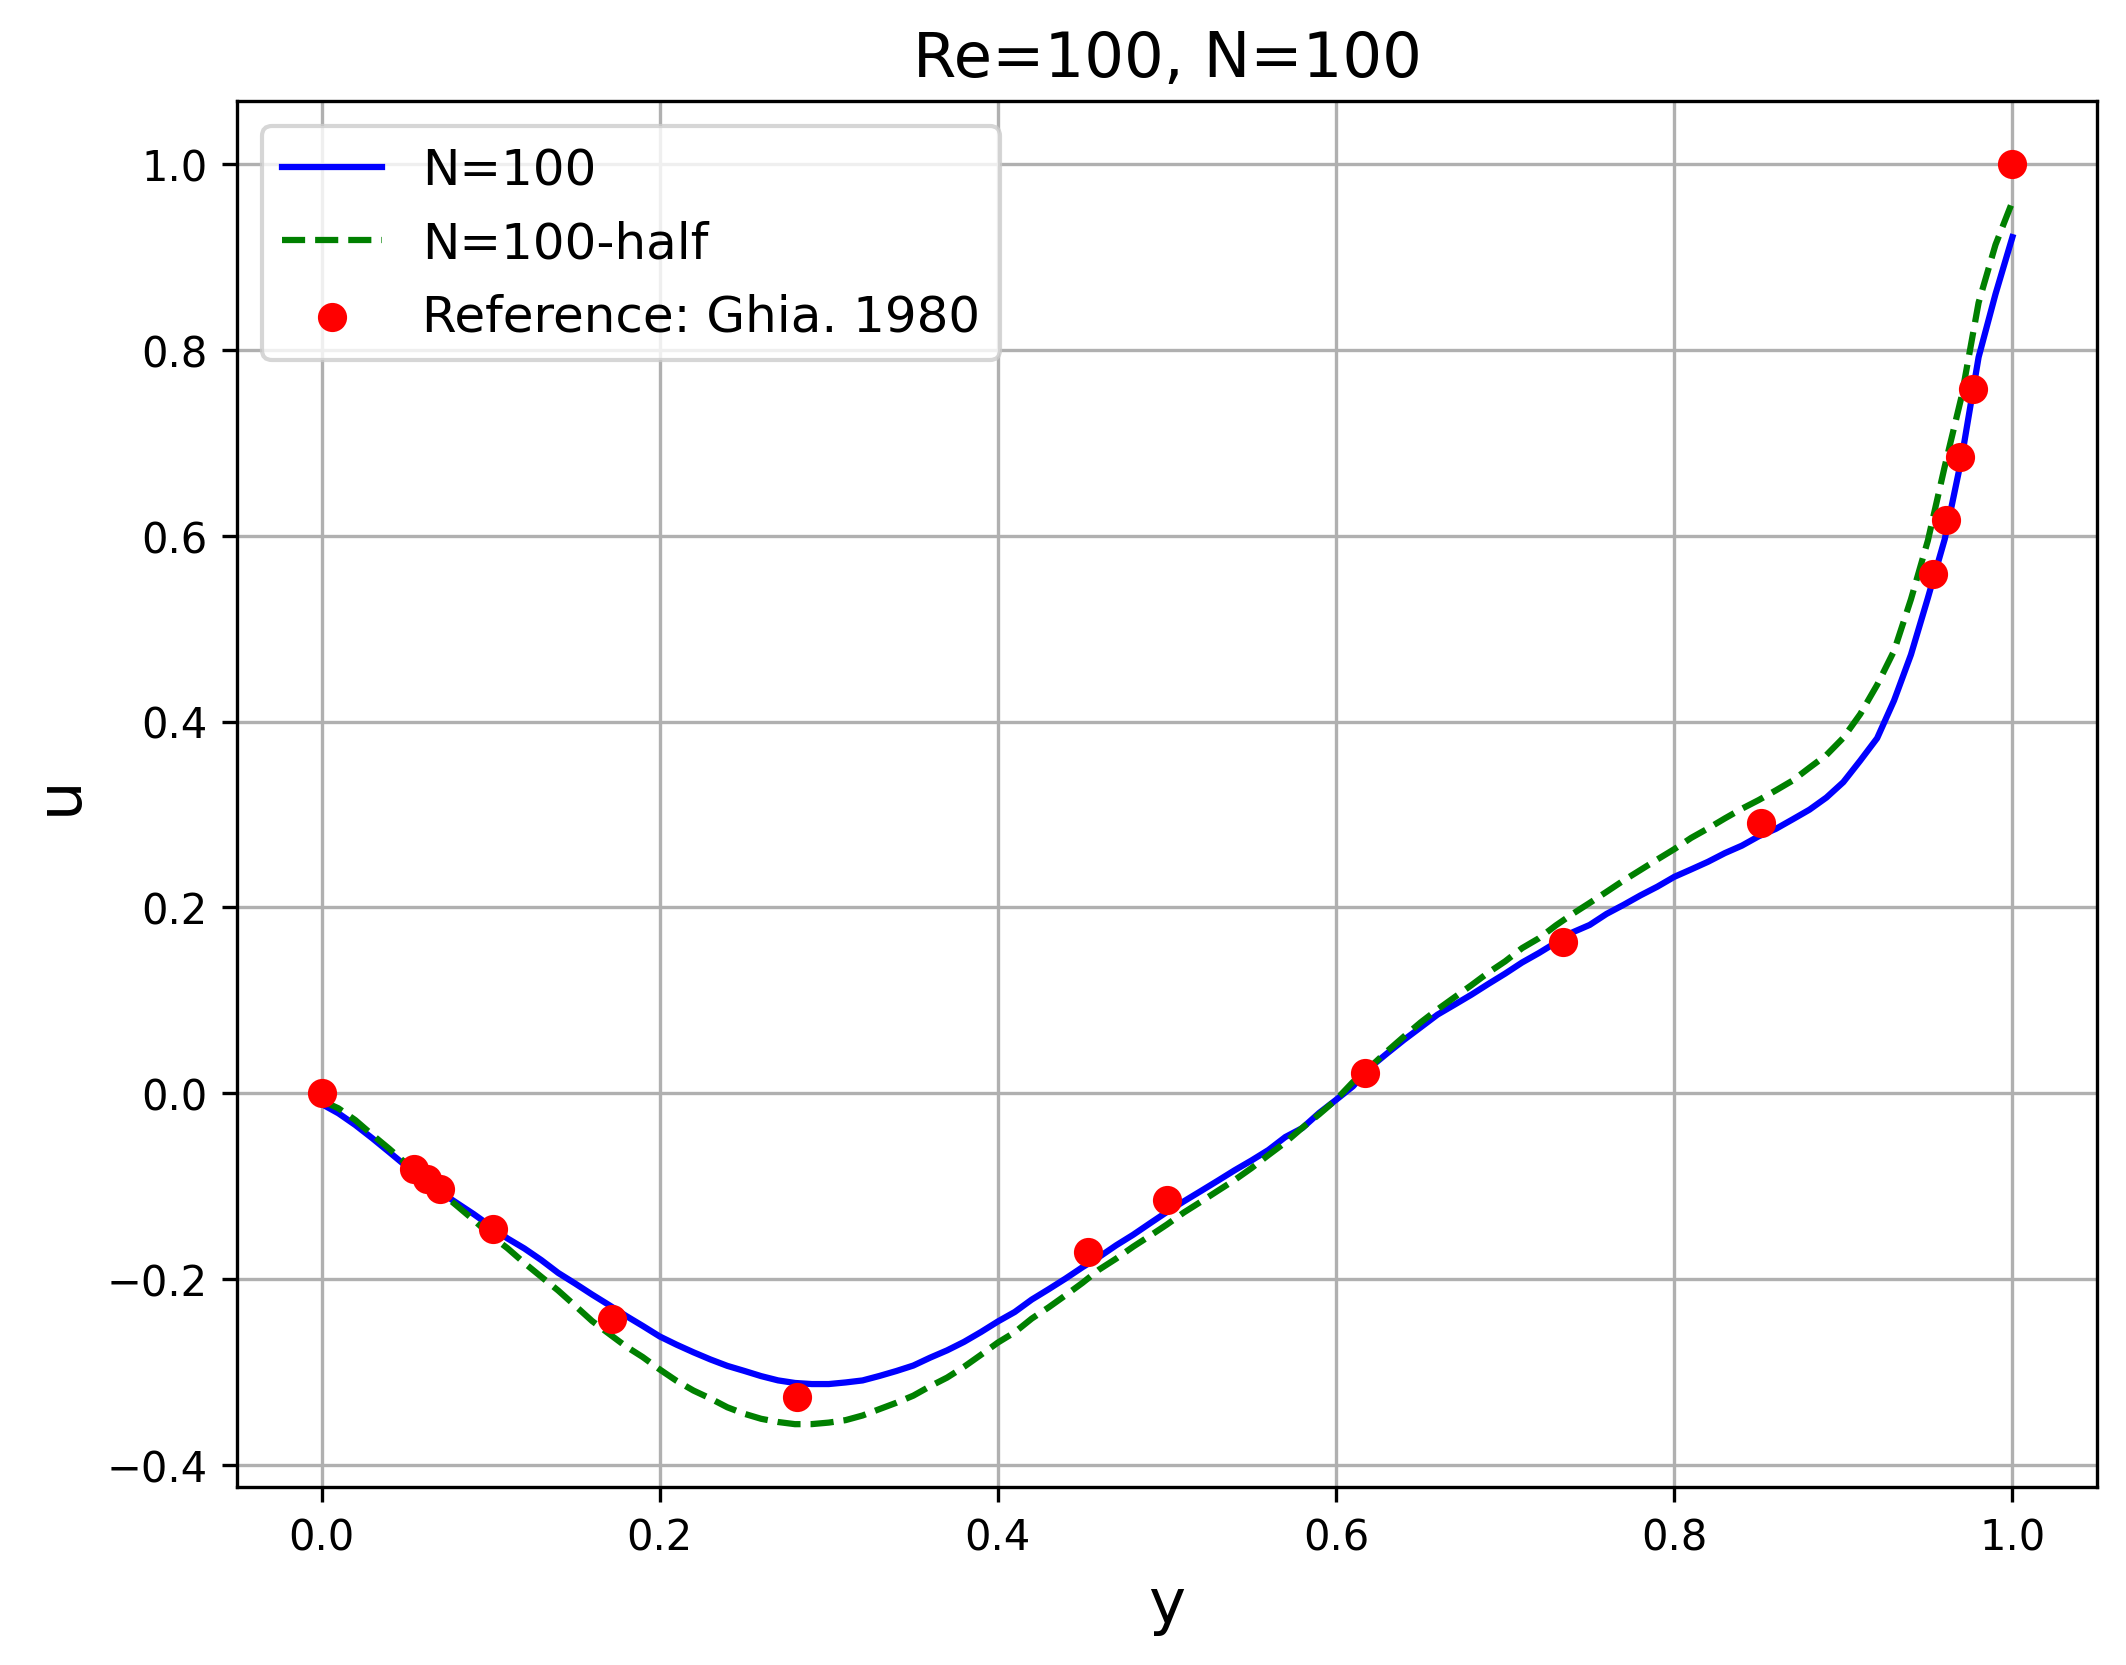
\includegraphics[width=0.45\textwidth]{images/LidDrivenCavity/Re400/u_middle_re400_N100.png}
        }
    \end{figure}
\end{frame}

\begin{frame}
    \begin{figure}[H]
        \centering
        \subfigure[$N=50$]{
            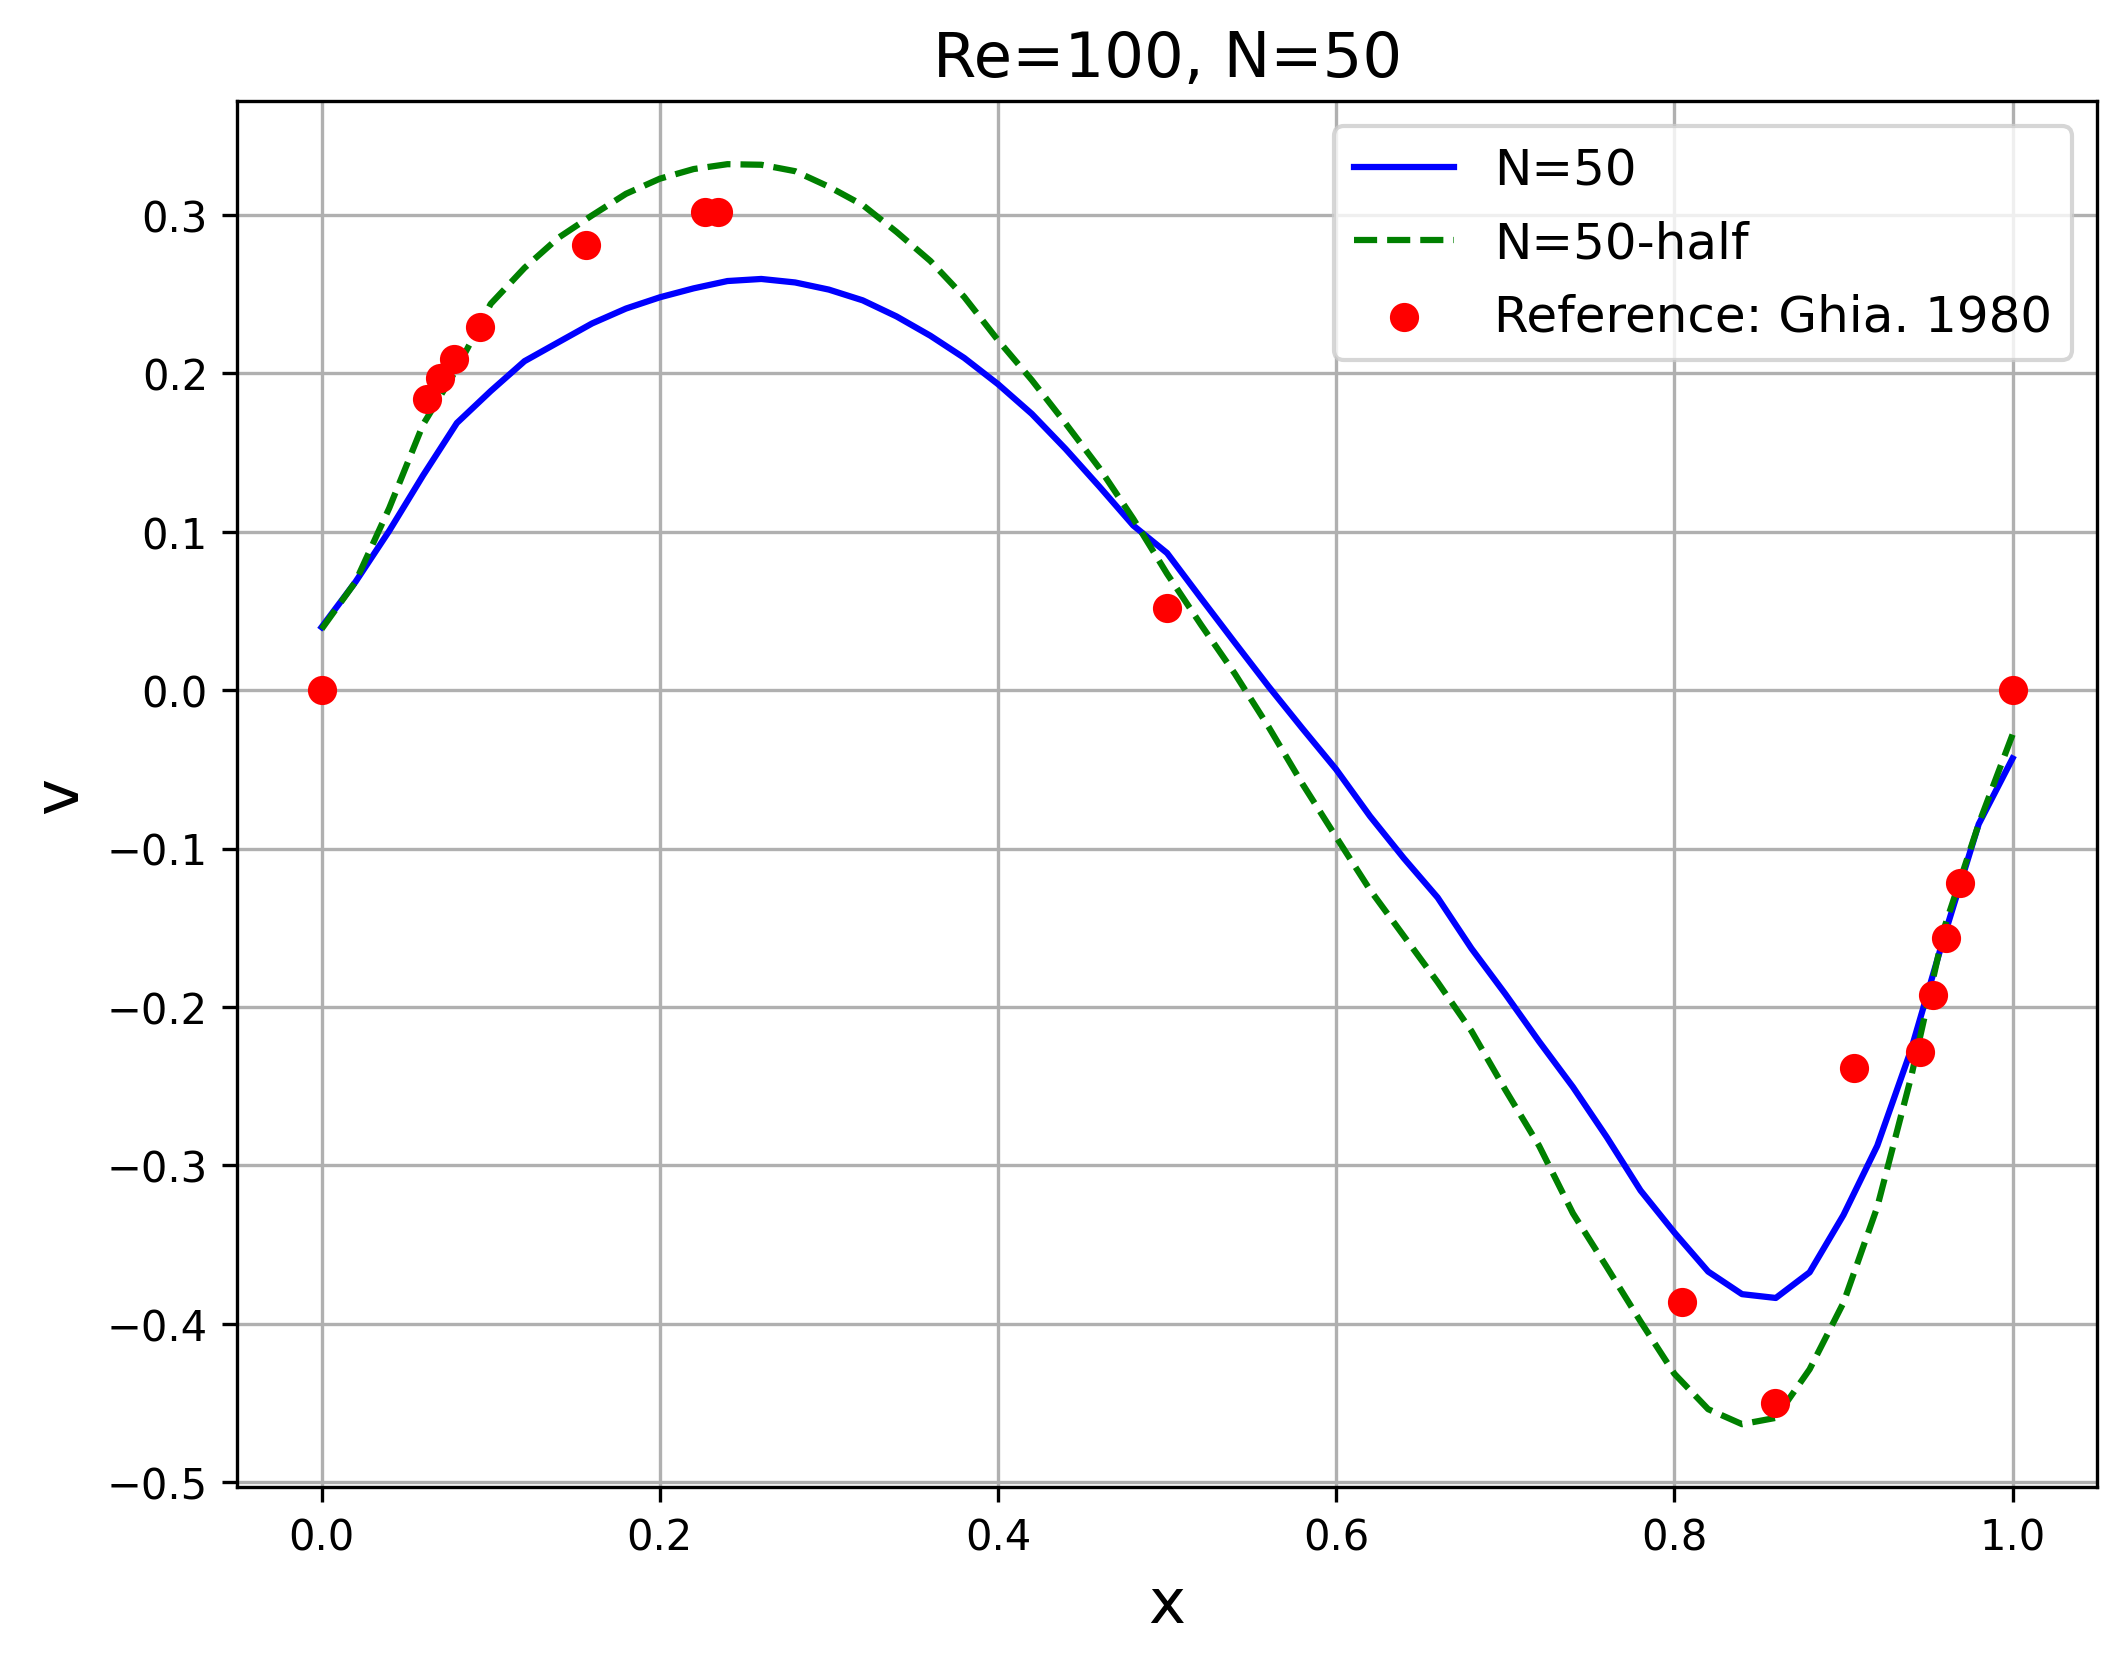
\includegraphics[width=0.45\textwidth]{images/LidDrivenCavity/Re400/v_middle_re400_N50.png}
        }
        \subfigure[$N=100$]{
            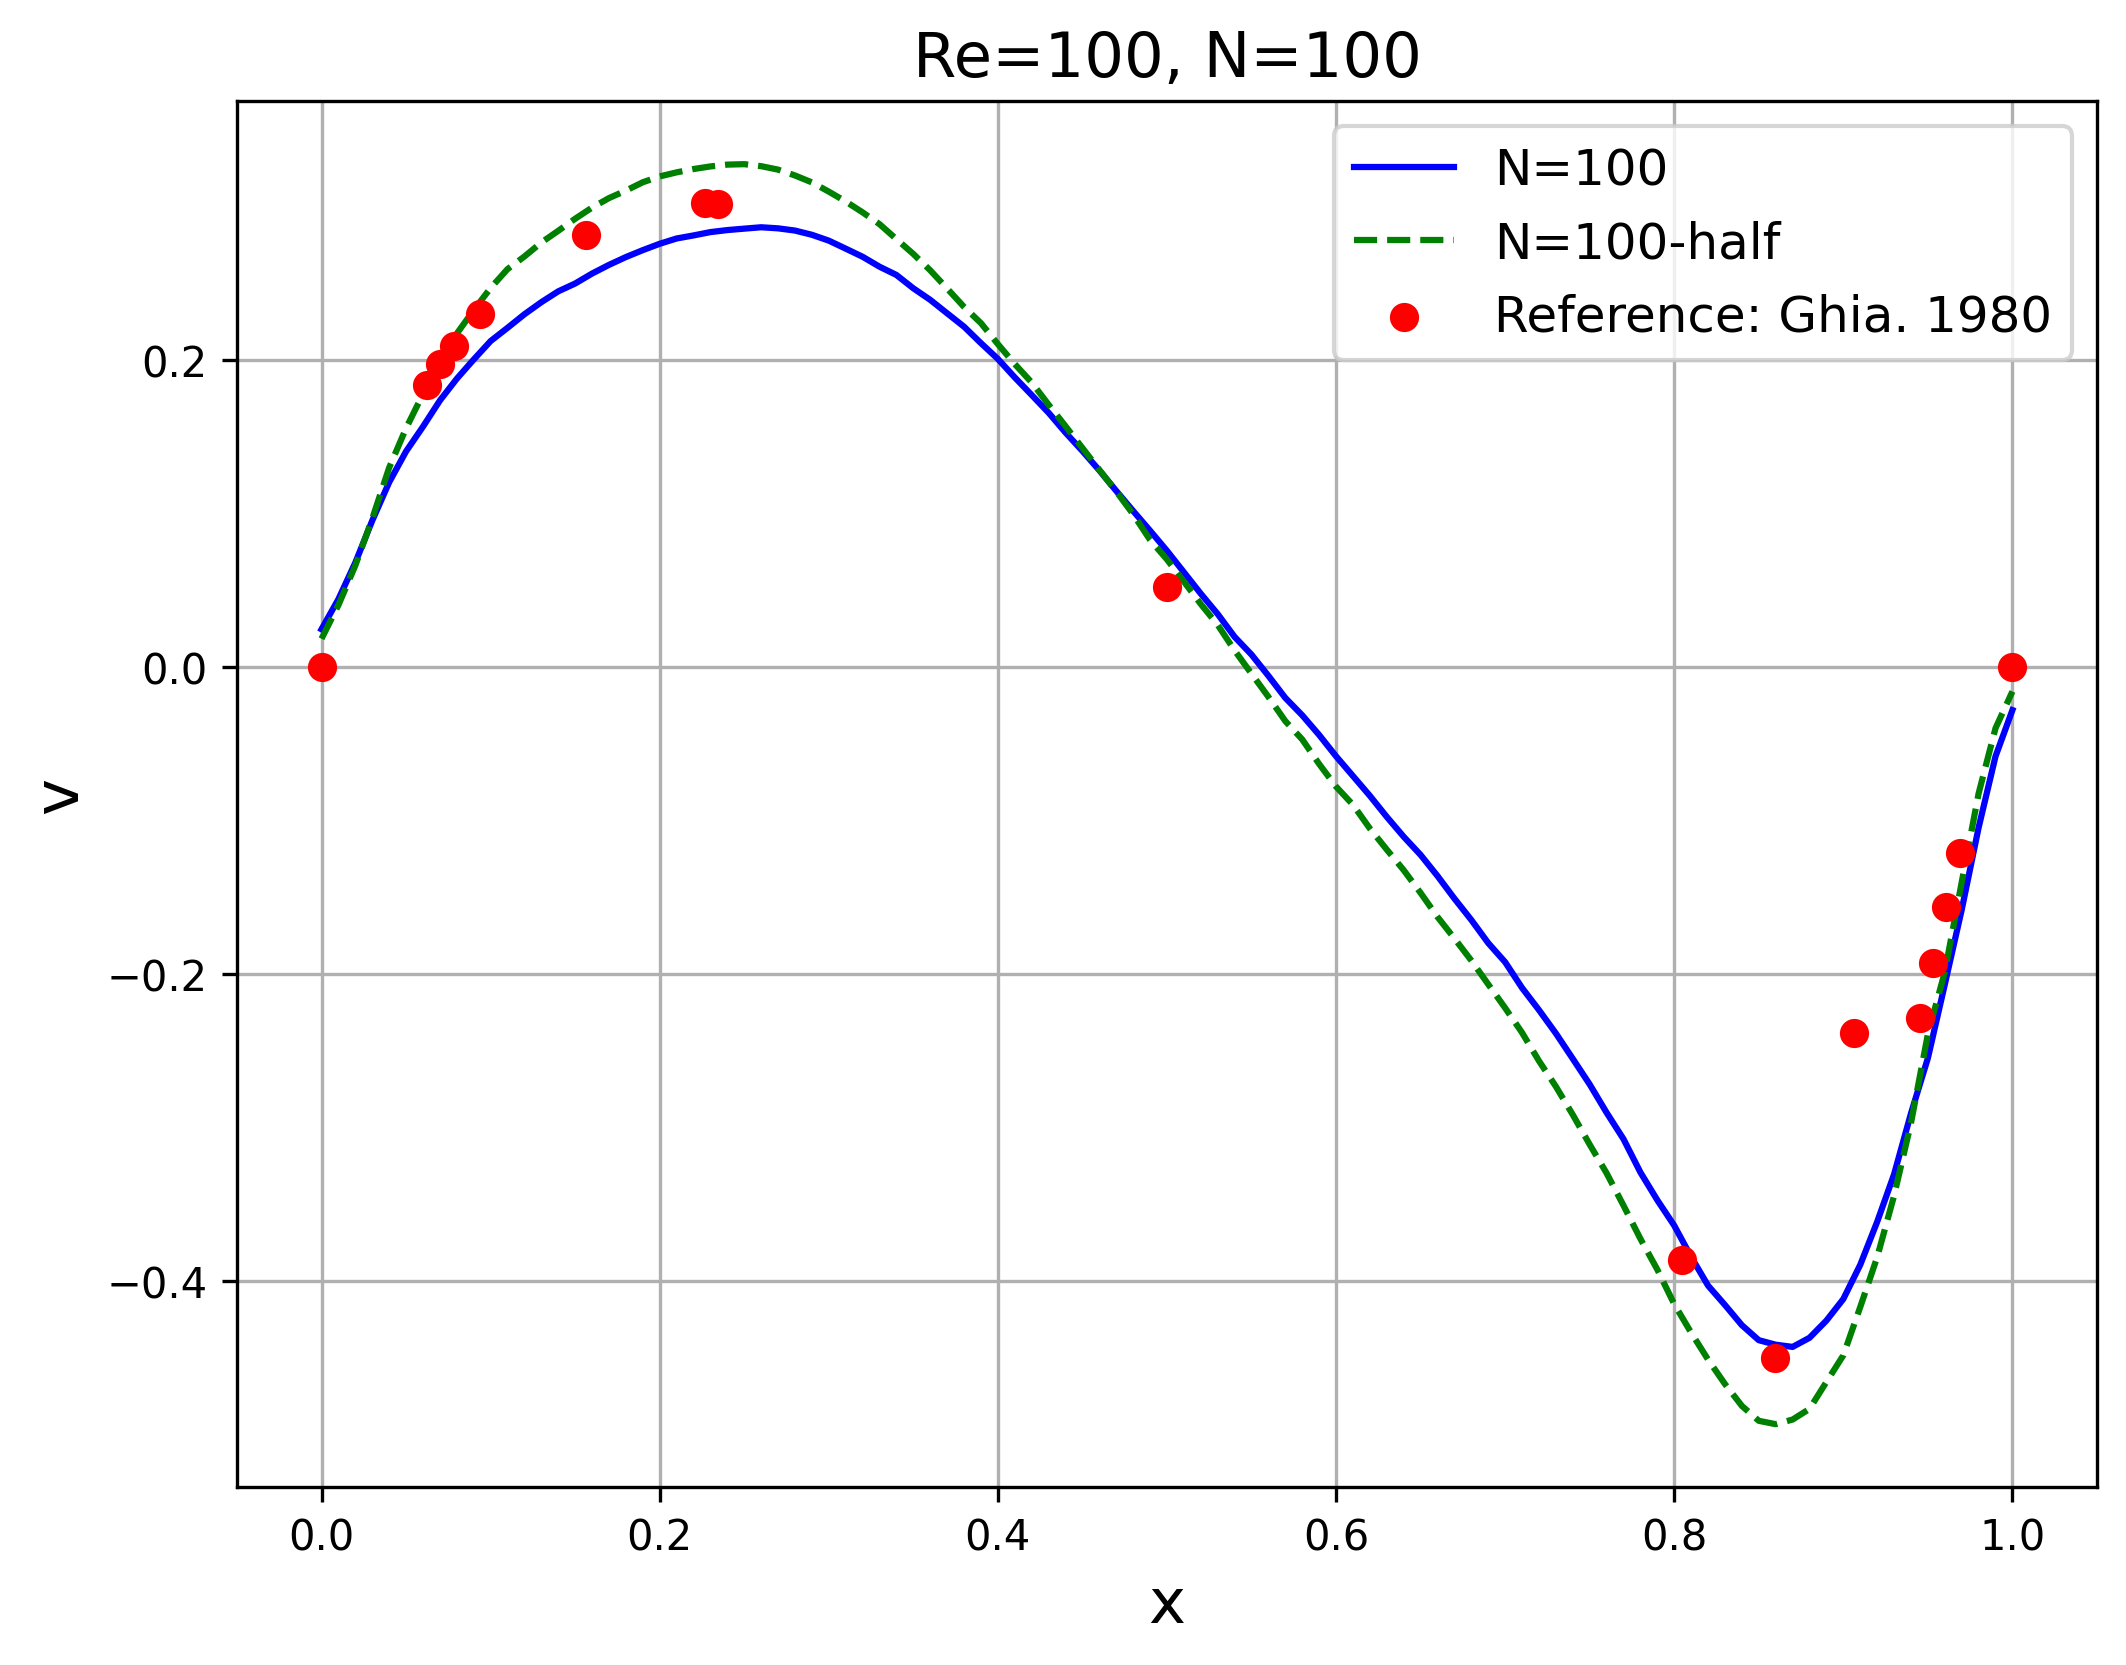
\includegraphics[width=0.45\textwidth]{images/LidDrivenCavity/Re400/v_middle_re400_N100.png}
        }
    \end{figure}
\end{frame}

\begin{frame}
    对于顶盖驱动流而言:
    \begin{itemize}
        \item 不垫高壁面粒子,会导致边界处流速仍不为零,并且增加粒子数的精度增益不明显。
        \item 垫高壁面粒子,会导致流域内部速度偏差稍大,但边界处的流速更吻合于边界设定值。
    \end{itemize}
\end{frame}
\section{泊肃叶流}

\begin{frame}
    \begin{figure}[H]
        \centering
        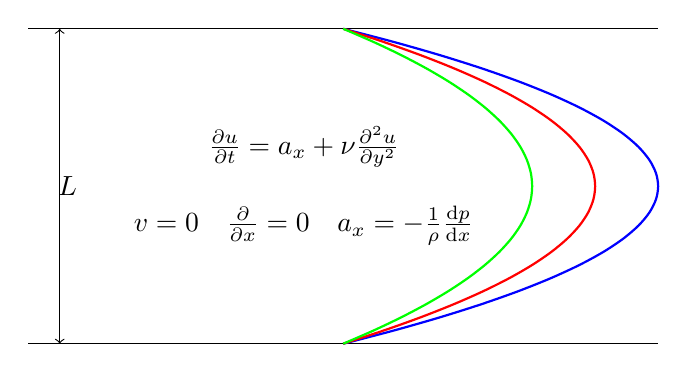
\begin{tikzpicture}
            \def\pipediameter{4}
            \def\pipelength{8}
            \draw (0,0) -- (\pipelength,0);
            \draw (0,\pipediameter) -- (\pipelength,\pipediameter);

            % \draw a y(L-y) = x inside the pipe
            % flow's shape
            \draw[domain=0:\pipediameter,smooth,variable=\y,blue,thick=3] plot ({4+\y*(\pipediameter-\y)},{\y});
            \draw[domain=0:\pipediameter,smooth,variable=\y,red,thick=3] plot ({4+0.8*\y*(\pipediameter-\y)},{\y});
            \draw[domain=0:\pipediameter,smooth,variable=\y,green,thick=3] plot ({4+0.6*\y*(\pipediameter-\y)},{\y});
            
            % governing equation
            \node at (3.5,2.5) {$\frac{\partial u}{\partial t}  = a_x + \nu\frac{\partial^2 u}{\partial y^2}$};
            \node at (3.5,1.5) {$v=0\quad\frac{\partial }{\partial x}=0\quad a_x=-\frac{1}{\rho}\frac{\mathrm{d}p}{\mathrm{d}x}$};

            % L
            \node at (0.5, 0.5*\pipediameter) {$L$};
            \draw[<->] (0.4,0) -- (0.4,\pipediameter);
        \end{tikzpicture}
    \end{figure}
    级数解 (Morris):
    \begin{equation}
        \begin{aligned}
            u(y,t)
        &=
        \frac{a_x}{2\nu}y(L-y)\\
        &-
        \sum_{k=0}^{\infty}
        \frac{2a_xL^2}{\nu\pi^3(2k+1)^3}
        \sin\left(\frac{\pi(2k+1)y}{L}\right)
        \exp\left(-\frac{\pi^2(2k+1)^2\nu t}{L^2}\right)
        \end{aligned}
    \end{equation}
\end{frame}

\begin{frame}
    \begin{figure}[H]
        \centering
        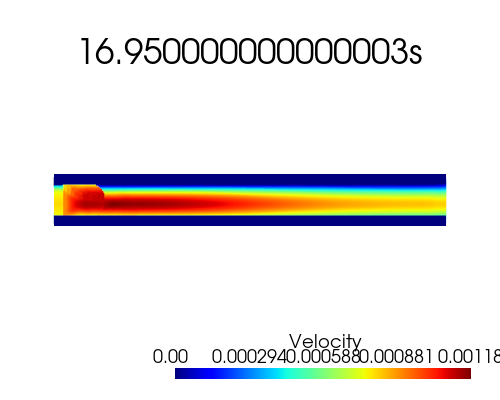
\includegraphics[width=0.8\textwidth]{images/Poiseuille2D/poiseuille_2d.png}
    \end{figure}
\end{frame}

\begin{frame}
    对于这种开边界问题,
    最常用的是采用“粒子缓冲区”技术进行处理。
    \begin{figure}[H]
        \centering
        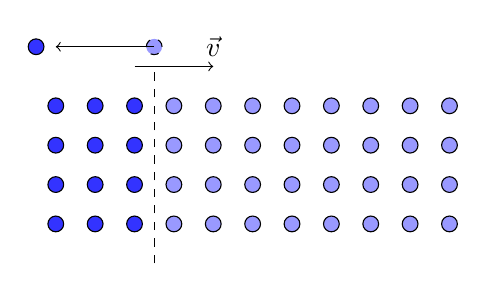
\begin{tikzpicture}
            % calculation domain
            % 8 * 4 particles
            % dx = 0.5
            \def\dx{0.5}
            \foreach \x in {0,1,...,7}
            \foreach \y in {0,1,...,3}
            \filldraw[fill=blue!40!white,draw=black] ({\x*\dx},{\y*\dx}) circle (0.1);
            % left inlet buffer
            \foreach \x in {-1,-2,-3}
            \foreach \y in {0,1,...,3}
            \filldraw[fill=blue!80!white,draw=black] ({\x*\dx},{\y*\dx}) circle (0.1);

            \draw[dashed] ({-\dx/2}, -\dx) -- ({-\dx/2}, 4*\dx);

            \draw[->] (-\dx, {4*\dx}) -- (\dx, {4*\dx}) node[above] {$\vec{v}$};

            % draw a particle pass into calcilation domain with dashed line
            \filldraw[fill=blue!40!white,draw=black,dashed] ({-\dx/2},{4.5*\dx}) circle (0.1);
            % draw a circle line to let the particle back to the buffer
            \draw[->] ({-\dx/2},{4.5*\dx}) -- ({-\dx/2-2.5*\dx},{4.5*\dx});
            \filldraw[fill=blue!80!white,draw=black] ({-\dx/2-3*\dx},{4.5*\dx}) circle (0.1);
        \end{tikzpicture}
    \end{figure}
    一旦 inlet 流入区域的粒子跨过了缓冲区的边界,
    则将其实例化成一个新流体粒子纳入计算区域。
    而将其位置重新沿流向,上溯缓冲区的宽度的距离,
    重新放入缓冲区。
    而另一方面流出区域的粒子则直接删除,也会有一个 outlet 缓冲区。

    因此泊肃叶流中,
    需要有:壁面粒子,流入缓冲区粒子,计算区域粒子,流出缓冲区粒子。
\end{frame}

\begin{frame}
    \begin{figure}[H]
        \centering
        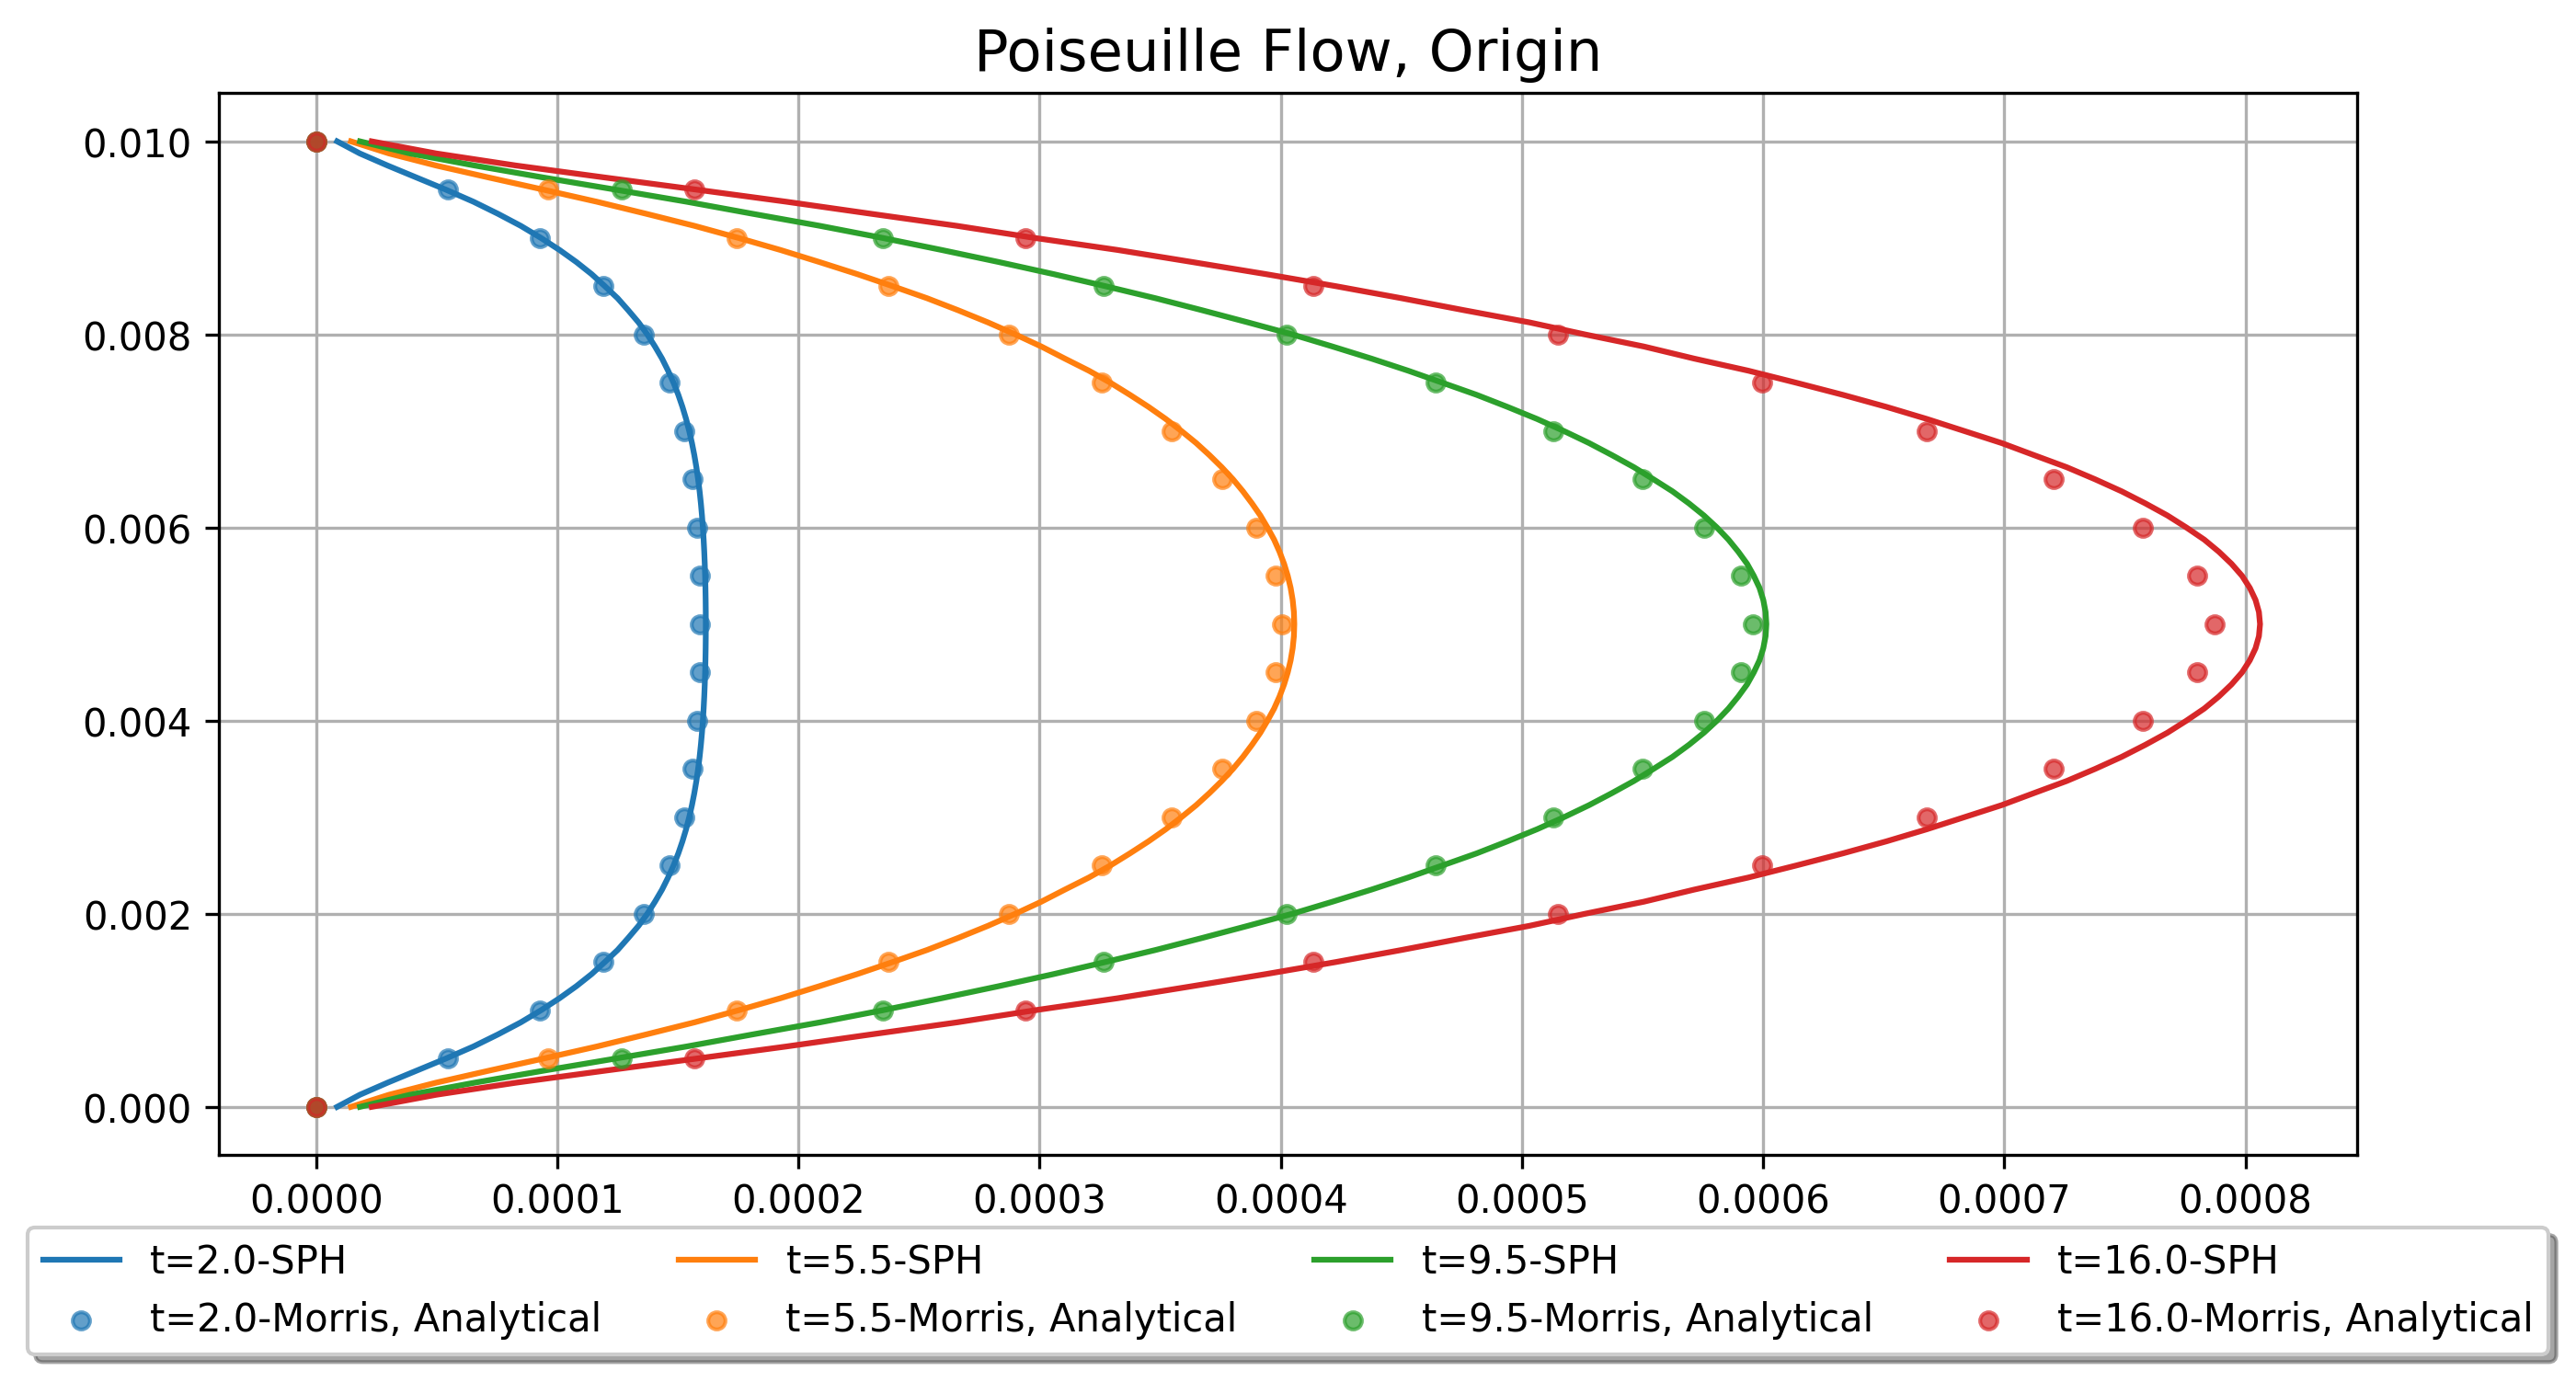
\includegraphics[width=\textwidth]{images/Poiseuille2D/poiseuille_2d_origin.png}
        \caption{未垫高壁面粒子的泊肃叶流}
    \end{figure}
\end{frame}

\begin{frame}
    \begin{figure}[H]
        \centering
        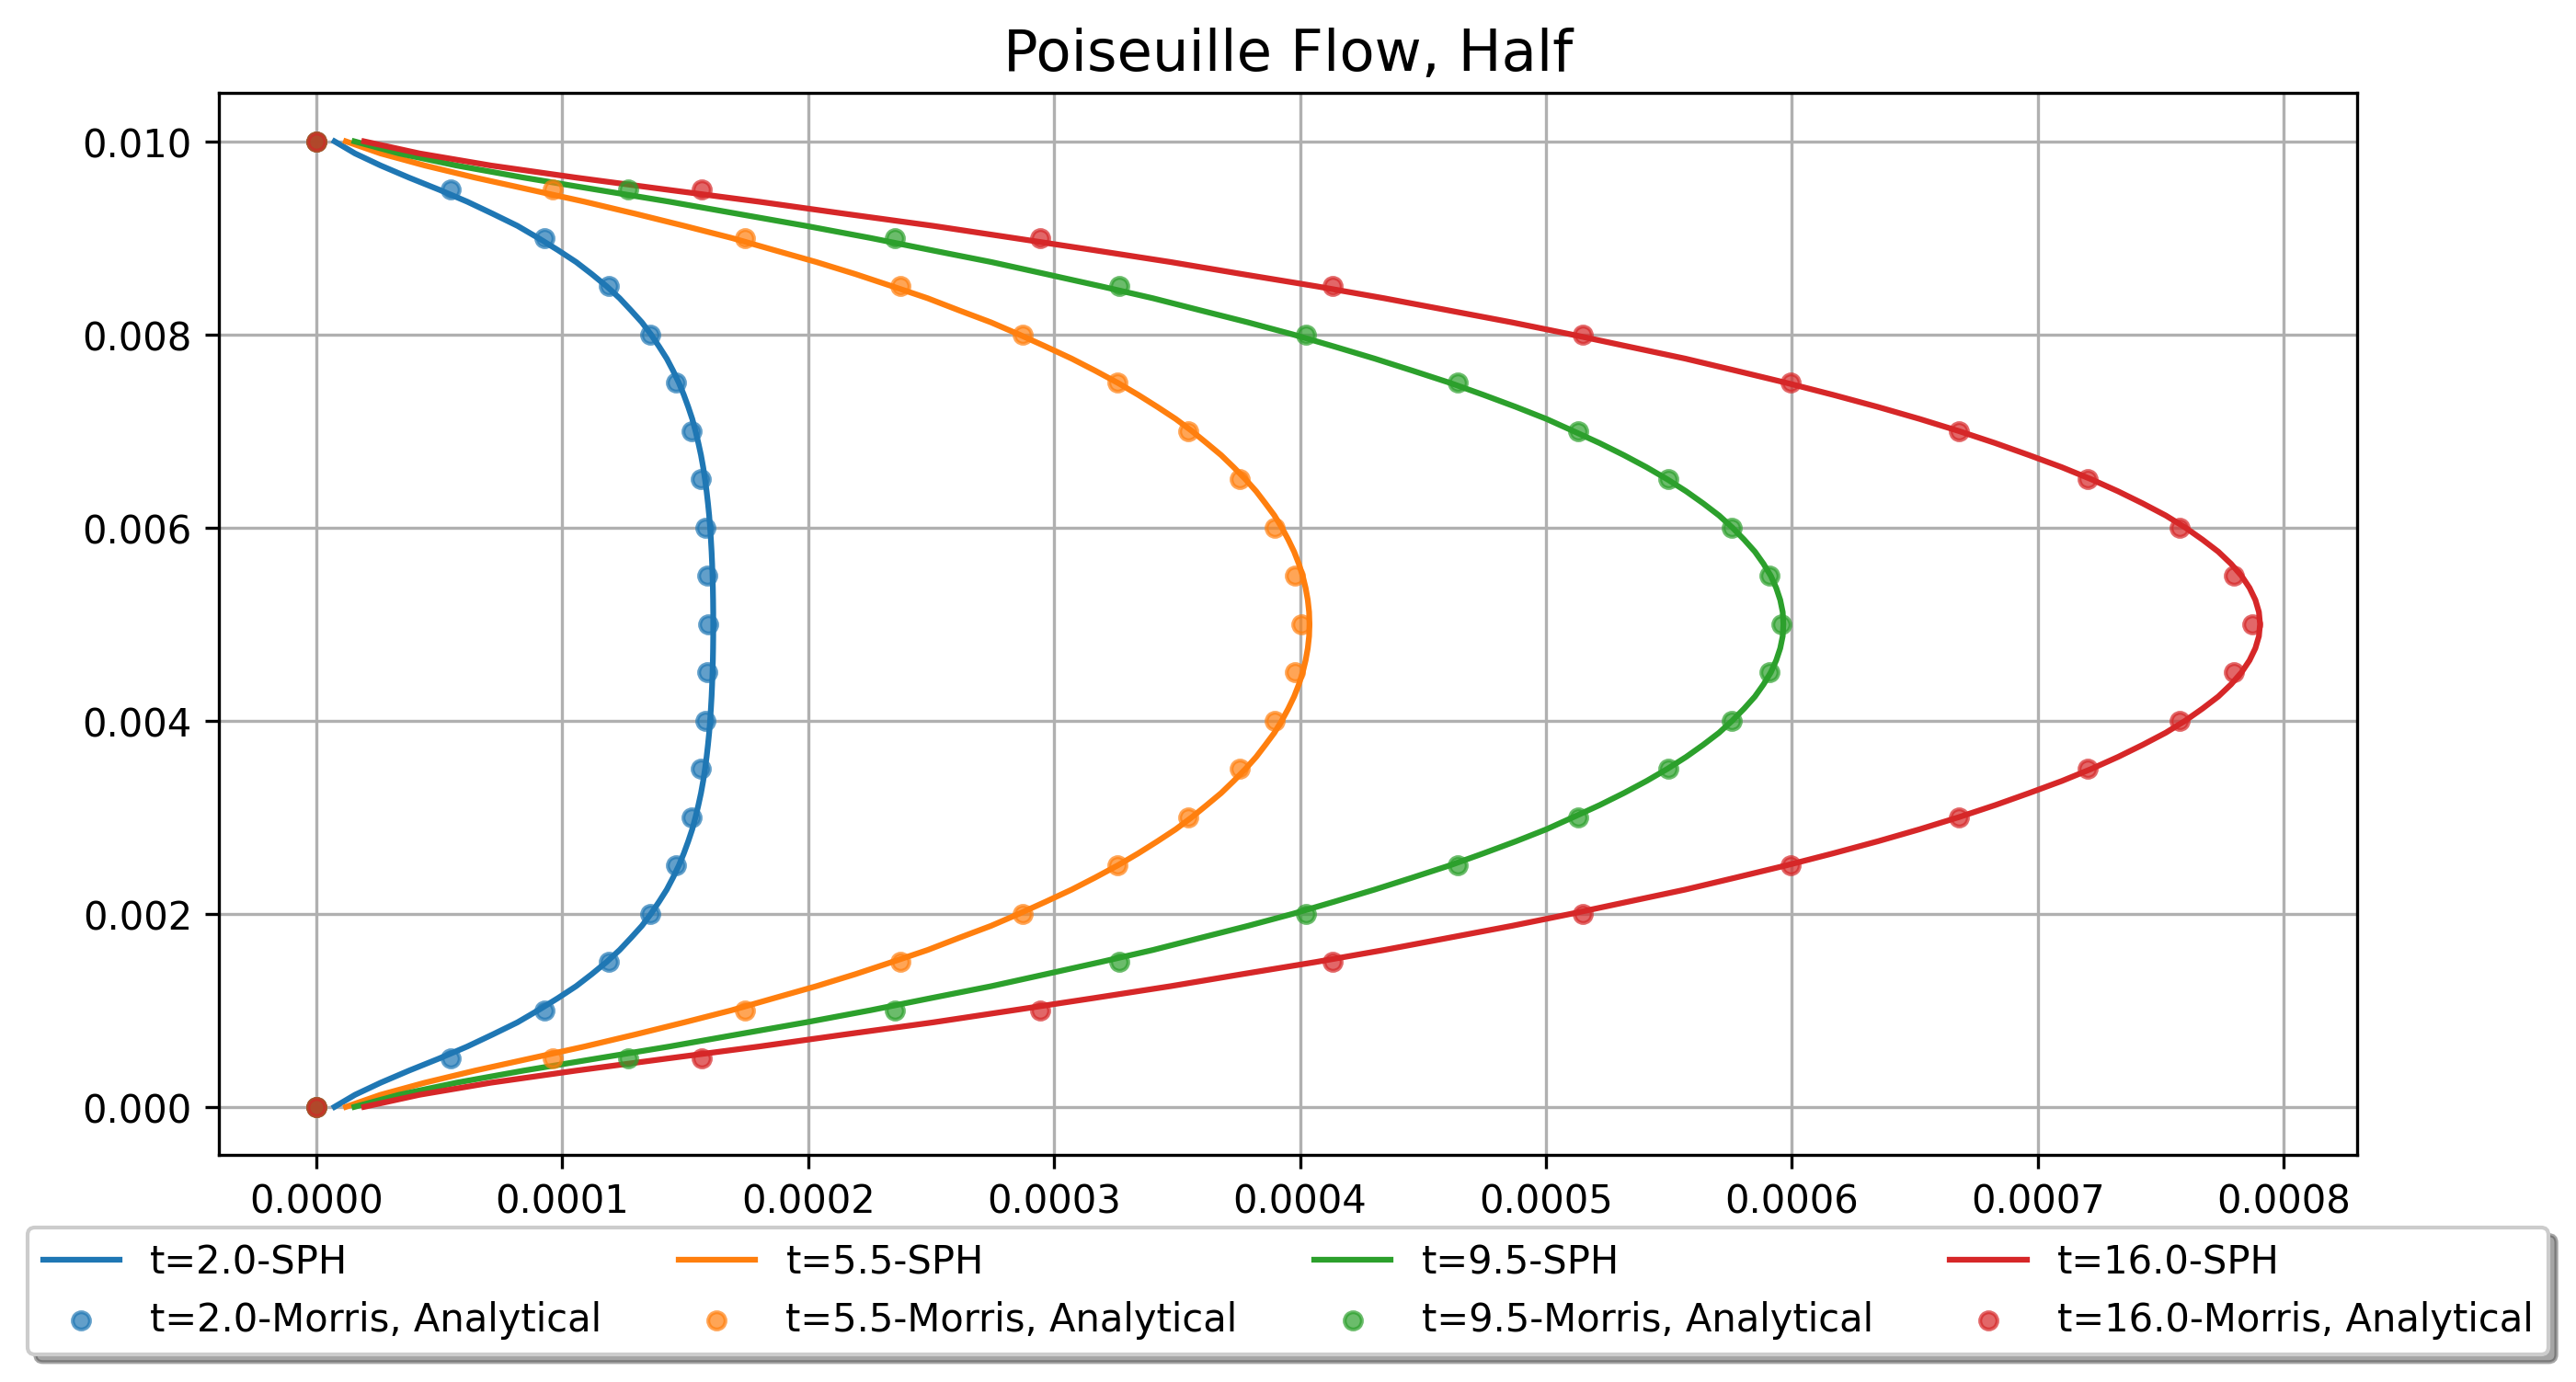
\includegraphics[width=\textwidth]{images/Poiseuille2D/poiseuille_2d_half.png}
        \caption{垫高壁面粒子的泊肃叶流}
    \end{figure}
\end{frame}

\begin{frame}
    通过泊肃叶流这个算例,
    可以发现垫高壁面粒子可以取得
    与理论解析解更加吻合的结果。
    
    但是似乎在顶盖驱动流算例中却不是这样的。

    对于壁面摩擦这件事情,
    我查的论文中对粘性项的讨论都莫衷一是,
    而且 Monaghan 本人也认为 SPH 中的壁面条件是一个并没有完全解决的问题。
    (包括开边界中如何正确利用黎曼条件)。
    不过至少目前看来,
    垫高壁面粒子是一个可行的方案。
\end{frame}
\section{其他技术的讨论}

\subsection{XSPH 方法}

\begin{frame}
    在之前的程序中,
    XSPH 方法被采用:
    \begin{equation}
        \frac{\mathrm{d}\vec{r}_i}{\mathrm{d}t}=
        \vec{v}_i-
        \epsilon\sum_j
        \frac{m_j}{\rho_j}
        \vec{v}_{ij}W_{ij}
    \end{equation}
    但该方法仅限于层流求解,
    并不适用于开放水体的求解。
    比如流体回注入水槽的时候,
    若采用 XSPH 会导致平稳水面被注入流体破坏,
    甚至很容易产生异常负压区,进而发生数值不稳定。


    但是对于泊肃叶流和顶盖驱动流类似算例,
    采用 XSPH 方法确实可以得到较好的结果。
\end{frame}

\subsection{$\delta^+$ SPH 密度修正器}

\begin{frame}

$\delta^+$ SPH 密度修正器可以有效地稳定密度场,进而稳定压力场。

\begin{equation}
    \left(
        \frac{\partial \rho}{\partial t}
    \right)_i
    =
    \sum_j m_j \vec{u}_{ij} \cdot \nabla W_{ij}
    +
    h c_0 \delta
    \sum_j  \frac{m_j}{\rho_j} \vec{D}_{ij}\cdot \nabla W_{ij}
\end{equation}
$\vec{D}_{ij}$ 计算如下。 首先提出一个核修正矩函数:
$[L]_i$ :
\begin{equation}
    [L]_i = \left[\sum_j \frac{m_j}{\rho_j}\vec{r}_{ij}\nabla W_{ij}\right]^{-1}
\end{equation}
$[L]_i$ 是一个 $d\times d$ 的矩阵,$d$ 为维度。
粒子致密时等价于单位阵。
进而提出修正的密度梯度 $\nabla \rho_i^L$ :
\begin{equation}
    \nabla \rho_i^L = \sum_j \frac{m_j}{\rho_j}\rho_{ij}
    [L]_i \cdot \nabla W_{ij}
\end{equation}
最后由 $\vec{D}_{ij}$ 给出:
\begin{equation}
    \vec{D}_{ij} = 
    \left[
        2\rho_{ij} - 
        \left(
            \nabla \rho_i^L + \nabla \rho_j^L
        \right)\cdot \vec{r}_{ij}
    \right]
    \frac{\vec{r}_{ij}}{r_{ij}^2 + 0.01h^2}
\end{equation}
\end{frame}

\begin{frame}
    $\delta$ 是一个无量纲参数,通常被设定为 $0.1$.
Monaghan 提出了一个修正器,可以有效地稳定密度场,进而稳定压力场。

$\delta^+$ SPH 模型有时甚至可以在弱可压(WCSPH)情形下给出比不可压(ICSPH)更好的结果。


我也在程序中实现了该修正器,
但不幸的是这个修正器对于计算量的增加是非常大的,
大约二位情形下会有 $6$ 倍的计算消耗提升,
这也可能是 SPH 方法不利用速度一阶导计算速度二阶导的原因(会涉及到两次邻域插值过程,对计算消耗很大)。

\begin{equation}
    \rho_i = \frac{\sum_j m_j W_{ij}}{\sum_j \frac{m_j}{\rho_j}W_{ij}}
\end{equation}

相对而言,频繁地使用上述核函数修正来稳定密度场可能从效果来看更好,
在实践中
$\delta^+$ 似乎学术意义大于其实际价值。
\end{frame}

\subsection{未来的工作安排}

\begin{frame}
    预计未来的工作计划:
    \begin{itemize}
        \item 打算上并行,在思考 CUDA 或者 MPI 的改版程序,现在的计算效率问题很大;
        \item 对于不同问题考虑不同的壁面摩擦,而不是用统一的壁面粘性模型,甚至可以自己提出一种壁面模型;
        \item 考虑不同的问题,比如传热等,物料或者多相流问题等。
        \item ...
    \end{itemize}
    *目前个人最想做的是改一个更强的并行版,现在的线程并行虽然有一定的效率,
    但遇到三维的大规模粒子计算还是捉襟见肘。
    
    *另外我觉得 Cruchaga 给的实验结果是非常好的算例比较,
    只要提出的壁面模型能和其实验值吻合,
    那么就能说明摩擦模型的可行性,
    进而用于更多的问题。
\end{frame}

\end{document}